% !TeX program = xelatex
\documentclass[11pt,a4paper]{article}

% -------------------------------------------------
% Packages
% -------------------------------------------------
\usepackage{kotex}
\usepackage{fontspec}
\usepackage{amsmath,amssymb,bm,mathtools}
\usepackage[left=24mm,right=24mm,top=23mm,bottom=25mm]{geometry}
\usepackage{booktabs,array}
\usepackage{longtable}
\usepackage{enumitem}
\usepackage{setspace}
\usepackage{xcolor}
\usepackage{colortbl}
\usepackage{graphicx}
\usepackage{tikz}
\usepackage{pifont}
\usetikzlibrary{positioning,arrows.meta,calc,fit,decorations.pathreplacing,shapes.geometric,backgrounds}
\usepackage[most]{tcolorbox}
\usepackage{listings}
\usepackage{hyperref}
\usepackage{fancyhdr}

\setstretch{1.14}
\setlength{\parindent}{0pt}
\setlength{\parskip}{0.55em}
\setlength{\emergencystretch}{2em}   % long \texttt{...} words: stretch the line instead of overfull

% -------------------------------------------------
% Colors and boxes
% -------------------------------------------------
\definecolor{deepblue}{RGB}{34,71,120}
\definecolor{softblue}{RGB}{239,246,253}
\definecolor{softgray}{RGB}{246,247,249}
\definecolor{softgreen}{RGB}{239,249,242}
\definecolor{softyellow}{RGB}{255,249,229}
\definecolor{codegray}{RGB}{248,248,248}

\newtcolorbox{keybox}[1][]{
  colback=softblue,
  colframe=deepblue,
  boxrule=0.7pt,
  arc=2mm,
  title=#1,
  fonttitle=\bfseries
}

\newtcolorbox{thinkbox}[1][]{
  colback=softyellow,
  colframe=orange!70!black,
  boxrule=0.6pt,
  arc=2mm,
  title=#1,
  fonttitle=\bfseries
}

\newtcolorbox{remarkbox}[1][]{
  colback=softgray,
  colframe=black!45,
  boxrule=0.5pt,
  arc=2mm,
  title=#1,
  fonttitle=\bfseries
}

\newtcolorbox{mlbox}[1][]{
  colback=softgreen,
  colframe=green!45!black,
  boxrule=0.6pt,
  arc=2mm,
  title=#1,
  fonttitle=\bfseries
}

% -------------------------------------------------
% Code style
% -------------------------------------------------
\lstdefinestyle{pythonstyle}{
  language=Python,
  backgroundcolor=\color{codegray},
  basicstyle=\ttfamily\small,
  keywordstyle=\bfseries,
  commentstyle=\itshape\color{black!60},
  stringstyle=\color{black!75},
  numbers=left,
  numberstyle=\tiny\color{black!55},
  numbersep=8pt,
  frame=single,
  rulecolor=\color{black!25},
  breaklines=true,
  showstringspaces=false,
  tabsize=4,
  columns=fullflexible,
  keepspaces=true
}
\lstset{style=pythonstyle}

% -------------------------------------------------
% Photos: a gray box is drawn if the file is missing
% \photo{file}{width}{caption}
% -------------------------------------------------
\newcommand{\photo}[3]{%
\begin{minipage}[b]{#2}\centering
\IfFileExists{figures/photos/#1}%
  {\includegraphics[width=\linewidth,height=0.3\textheight,keepaspectratio]{figures/photos/#1}}%
  {\fbox{\parbox[c][0.55\linewidth][c]{0.95\linewidth}{\centering\small\ttfamily\detokenize{#1}}}}\\[0.2em]
{\small #3}
\end{minipage}}

% -------------------------------------------------
% Math commands
% -------------------------------------------------
\newcommand{\R}{\mathbb{R}}
\newcommand{\T}{^{\mathsf T}}

% -------------------------------------------------
% Header / footer
% -------------------------------------------------
\pagestyle{fancy}
\fancyhf{}
\lhead{Introduction to Deep Learning and Practice}
\rhead{Reading: Hardware for Deep Learning}
\cfoot{\thepage}
\renewcommand{\headrulewidth}{0.4pt}
\setlength{\headheight}{14pt}

\hypersetup{
  colorlinks=true,
  linkcolor=deepblue,
  urlcolor=deepblue
}

% =================================================
% =================================================
\begin{document}
% =================================================

\begin{center}
{\LARGE\bfseries 딥러닝 개발자를 위한 하드웨어}\\[0.3em]
{\large (Hardware for Deep Learning) \quad 읽기 자료}\\[0.5em]
{\normalsize CPU와 메모리 $\cdot$ PCIe $\cdot$ GPU의 내부 $\cdot$ 숫자 형식 $\cdot$ 성능 지표 $\cdot$ GPU의 세대 $\cdot$ 개발 환경}\\[0.8em]
\end{center}

\begin{keybox}[이 읽기 자료의 핵심 질문]
딥러닝 노트 3절에서 학습 시간의 대부분이 행렬곱이고, GPU가 그것을 빠르게 한다는 것을 보았다.
그런데 GPU 사양표에는 SM, CUDA core, tensor core, GDDR7, HBM3e, TFLOPS, PCIe 5.0 x16, TF32 같은 말이 가득하다.
이 말들은 각각 무엇을 뜻하는가? 내 코드의 속도는 그중 무엇이 정하는가?
그리고 연구실에 GPU 컴퓨터를 들여놓는다면 무엇을 확인해야 하는가?
\end{keybox}

\subsection*{학습목표}

이 읽기 자료를 읽고 나면 다음을 설명할 수 있어야 한다.

\begin{enumerate}[label=\arabic*.]
\item 학습 데이터가 SSD에서 GPU의 계산 장치까지 가는 길과, 각 구간의 대역폭을 설명한다.
\item PCIe, lane, x16/x8, CPU 직결과 칩셋, M.2와 NVMe의 뜻을 메인보드 사진에서 찾아 설명한다.
\item RAM, DRAM, SRAM, DDR, GDDR, HBM의 이름의 뜻과 차이, D램과 낸드의 셀 구조와 성질의 차이, 그리고 대역폭과 지연시간의 차이를 설명한다.
\item GPU 안의 SM, CUDA core, tensor core, warp의 관계를 설명하고, 사양표의 TFLOPS를 계산으로 확인한다.
\item FP64, FP32, TF32, BF16, FP16, FP8의 비트 구조를 그리고, 속도와 정확도의 관계를 측정으로 보인다.
\item roofline model로 연산이 memory-bound인지 compute-bound인지 판단한다.
\item A100, H100, B200과 RTX 시리즈의 차이를 설명하고, 연구용 GPU 컴퓨터의 구성을 검토한다.
\end{enumerate}

\begin{remarkbox}[이 읽기 자료의 코드 (\texttt{code/} 폴더)]
\begin{tabular}{@{}ll@{}}
\texttt{device\_info.py} & GPU, SM 수, VRAM, compute capability, CUDA 버전 출력 \\
\texttt{gpu\_bench.py} & 행렬곱 속도와 정확도, VRAM과 PCIe의 대역폭 측정 \\
\texttt{hardware\_charts.py} & 대역폭 비교, GPU별 성능 그래프 (사양 값) \\
\end{tabular}
\medskip

\texttt{gpu\_bench.py}는 NVIDIA GPU와 PyTorch가 필요하다.
이 자료의 측정값은 강의자의 노트북 (\textbf{RTX 3050 4GB Laptop GPU}, 전력 한도 35 W)에서 얻은 것이다.
여러분의 GPU에서 실행하여 숫자를 비교해 보라.
\end{remarkbox}

% =================================================
\section{컴퓨터 한 대를 열어 보면}\label{sec:parts}
% =================================================

\subsection{부품과 역할}\label{sec:parts_roles}

딥러닝용 컴퓨터도 보통의 컴퓨터와 같은 부품으로 이루어진다. 다만 각 부품이 학습에서 맡는 역할을 알아야 어디가 병목인지 판단할 수 있다.

\begin{center}
{\small
\begin{tabular}{@{}>{\raggedright\arraybackslash}p{30mm}>{\raggedright\arraybackslash}p{52mm}>{\raggedright\arraybackslash}p{68mm}@{}}
\toprule
부품 & 하는 일 & 딥러닝에서의 의미 \\
\midrule
CPU & 프로그램 전체를 지휘한다 & 데이터 읽기와 전처리, GPU에 일 시키기. 계산 자체는 대부분 GPU가 한다 \\
메모리 (RAM) & CPU가 지금 쓰는 데이터를 둔다 & 데이터셋, 미니배치를 만드는 동안의 데이터. 보통 VRAM 합계의 $2$배 이상을 권한다 \\
저장장치 (SSD, HDD) & 전원이 꺼져도 남는 저장 & 데이터셋과 체크포인트. 데이터를 읽는 속도가 느리면 GPU가 논다 \\
GPU & 대량의 단순 계산을 동시에 & 행렬곱과 합성곱. 학습 속도의 대부분을 정한다 \\
VRAM & GPU 전용 메모리 & 모델의 매개변수, 기울기, 중간값. 용량이 모자라면 학습이 안 된다 \\
메인보드 & 부품을 꽂고 서로 잇는다 & GPU를 몇 장, 얼마나 넓은 통로 (PCIe lane)로 꽂을 수 있는가 \\
파워 (PSU) & 전기를 공급한다 & GPU 한 장이 수백 W를 쓴다. 용량이 모자라면 학습 중 꺼진다 \\
냉각 & 열을 뺀다 & 온도가 오르면 GPU가 스스로 클럭을 낮추어 (throttling) 느려진다 \\
\bottomrule
\end{tabular}}
\end{center}

다음 사진은 실제 부품이다. 2절 이후에 하나씩 자세히 본다.

\begin{center}
\photo{cpu_ryzen9_9950x_top.jpg}{0.31\textwidth}{CPU (AMD Ryzen 9 9950X, 윗면)}\hfill
\photo{ram_ddr5_dimm.jpg}{0.31\textwidth}{메모리 모듈 (DDR5 DIMM)}\hfill
\photo{ssd_m2_nvme.jpg}{0.31\textwidth}{M.2 NVMe SSD}\\[0.8em]
\photo{gpu_rtx5090_card.png}{0.31\textwidth}{그래픽카드 (RTX 5090)}\hfill
\photo{motherboard_atx_x570_top.jpg}{0.31\textwidth}{메인보드 (2.4절)}\hfill
\photo{psu_atx_corsair.jpg}{0.31\textwidth}{파워 서플라이 (PSU)}
\end{center}

\subsection{데이터가 지나는 길}\label{sec:datapath}

학습 한 step 동안 데이터는 다음 길을 지난다.

\begin{center}
\begin{minipage}{\textwidth}\centering
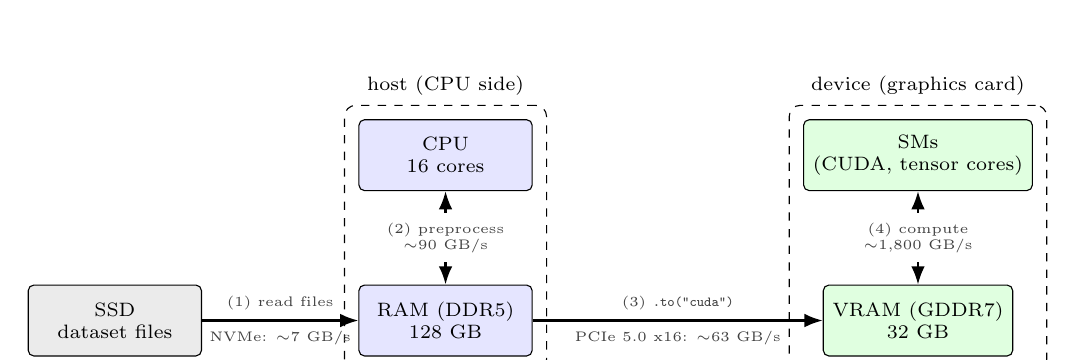
\begin{tikzpicture}[>=Latex,
  part/.style={draw,rounded corners=2pt,minimum width=22mm,minimum height=9mm,font=\scriptsize,align=center},
  lab/.style={font=\tiny,align=center,text=black!75}]
\node[part,fill=black!8] (ssd) at (0,-1.0) {SSD\\dataset files};
\node[part,fill=blue!10] (cpu) at (4.2,1.1) {CPU\\16 cores};
\node[part,fill=blue!10] (ram) at (4.2,-1.0) {RAM (DDR5)\\128 GB};
\node[part,fill=green!12] (sm) at (10.2,1.1) {SMs\\(CUDA, tensor cores)};
\node[part,fill=green!12] (vram) at (10.2,-1.0) {VRAM (GDDR7)\\32 GB};
\begin{scope}[on background layer]
\node[draw,dashed,rounded corners=4pt,fit=(cpu)(ram),inner sep=5pt,label={[font=\scriptsize]above:host (CPU side)}] (host) {};
\node[draw,dashed,rounded corners=4pt,fit=(sm)(vram),inner sep=5pt,label={[font=\scriptsize]above:device (graphics card)}] (gpu) {};
\end{scope}
\draw[->,thick] (ssd) -- node[lab,above] {(1) read files}node[lab,below] {NVMe: $\sim$7 GB/s} (ram);
\draw[<->,thick] (ram) -- node[lab,fill=white] {(2) preprocess\\$\sim$90 GB/s} (cpu);
\draw[->,thick] (ram) -- node[lab,above] {(3) \texttt{.to("cuda")}}node[lab,below] {PCIe 5.0 x16: $\sim$63 GB/s} (vram);
\draw[<->,thick] (vram) -- node[lab,fill=white] {(4) compute\\$\sim$1,800 GB/s} (sm);
\end{tikzpicture}

\small 학습 데이터가 지나는 길. 숫자는 한 방향의 대략적인 대역폭 (RTX 5090 컴퓨터의 예)이다.
\end{minipage}
\end{center}

\begin{enumerate}[label=(\arabic*)]
\item \textbf{파일 읽기.} 데이터셋 파일을 SSD에서 RAM으로 읽는다.
\item \textbf{전처리.} CPU가 이미지를 열고, 크기를 맞추고, 데이터 확장을 하여 미니배치를 만든다. PyTorch의 \texttt{DataLoader}가 이 일을 하고, \texttt{num\_workers}로 CPU 코어 여러 개를 쓴다.
\item \textbf{GPU로 복사.} 미니배치를 PCIe를 거쳐 VRAM으로 보낸다. 코드에서는 \texttt{xb.to(device)}이다.
\item \textbf{계산.} GPU의 계산 장치 (SM)가 VRAM에서 매개변수와 데이터를 읽어 순전파, 역전파, 갱신을 한다.
\end{enumerate}

이 길에서 가장 느린 구간이 전체 속도를 정한다. 구간마다 대역폭이 \textbf{수백 배}씩 다르다는 것에 주의하자.
VRAM과 SM 사이는 PCIe보다 약 $30$배 넓다. 그래서 학습 중에는 데이터를 GPU에 한 번 올린 뒤 GPU 안에서 최대한 많이 계산하는 것이 좋다.

\begin{thinkbox}[GPU가 놀고 있는지 확인하기]
학습 중 터미널에서 \texttt{nvidia-smi}를 실행하면 GPU 사용률 (GPU-Util)이 나온다.
이 값이 $100\%$에 가깝지 않고 들쭉날쭉하면, GPU가 (1)$\sim$(3)을 기다리고 있는 것이다.
\texttt{DataLoader(..., num\_workers=8, pin\_memory=True)}로 CPU 쪽 준비를 늘리거나, 데이터를 미리 전처리해 두면 빨라진다.
\end{thinkbox}

% =================================================
\section{메인보드와 PCIe}\label{sec:pcie}
% =================================================

\subsection{PCIe와 lane}\label{sec:lane}

\textbf{PCIe} (Peripheral Component Interconnect Express)는 메인보드 안에서 CPU와 그래픽카드, SSD 등을 잇는 \textbf{고속 데이터 통로의 규격}이다.
PCIe 통로는 \textbf{lane}이라는 단위로 이루어진다. lane 하나는 도로의 차선 하나와 같다.

\begin{itemize}[leftmargin=1.5em]
\item \textbf{x1, x4, x8, x16}: lane의 수이다. x16은 $16$차선이다. 그래픽카드 슬롯은 보통 x16 길이로 만들고, M.2 SSD는 x4를 쓴다.
\item \textbf{PCIe 3.0, 4.0, 5.0}: 세대이다. 세대가 하나 오르면 lane 하나의 속도가 약 $2$배가 된다.
\end{itemize}

\begin{center}
{\small
\begin{tabular}{@{}lccccl@{}}
\toprule
세대 (발표) & lane 하나 & x4 & x8 & x16 & 쓰이는 곳의 예 \\
\midrule
PCIe 3.0 (2010) & $\sim$1 GB/s & $\sim$4 & $\sim$8 & $\sim$16 GB/s & 오래된 컴퓨터 \\
PCIe 4.0 (2017) & $\sim$2 GB/s & $\sim$8 & $\sim$16 & $\sim$32 GB/s & RTX 30/40, A100, NVMe SSD \\
PCIe 5.0 (2019) & $\sim$4 GB/s & $\sim$16 & $\sim$32 & $\sim$63 GB/s & RTX 5090, H100, B200 \\
PCIe 6.0 (2022) & $\sim$8 GB/s & $\sim$32 & $\sim$63 & $\sim$121 GB/s & 최신 서버 \\
\bottomrule
\end{tabular}}

\small 한 방향의 대략적인 대역폭. 양방향으로 동시에 같은 양을 보낼 수 있다.
\end{center}

그래서 \textbf{PCIe 5.0 x8 $\approx$ PCIe 4.0 x16}이다. 차선이 절반이어도 차선마다 두 배 빠르면 같다.

\subsection{CPU 직결과 칩셋}\label{sec:chipset}

CPU가 직접 내줄 수 있는 lane의 수는 정해져 있다. 데스크톱 CPU (예: AMD Ryzen 9000)는 그래픽카드용으로 $16$개, SSD용으로 $4$개 정도이다.
나머지 장치 (USB, 랜, Wi-Fi, 추가 SSD)는 \textbf{칩셋} (chipset)이라는 보조 칩이 모아서 CPU에 잇는다.
칩셋은 본사 (CPU)와 거래처들 사이의 \textbf{중계소}이다. 칩셋과 CPU 사이에는 x4 하나뿐이어서, 칩셋에 달린 장치들이 이 통로를 \textbf{나누어 쓴다}.

\begin{center}
\begin{minipage}{\textwidth}\centering
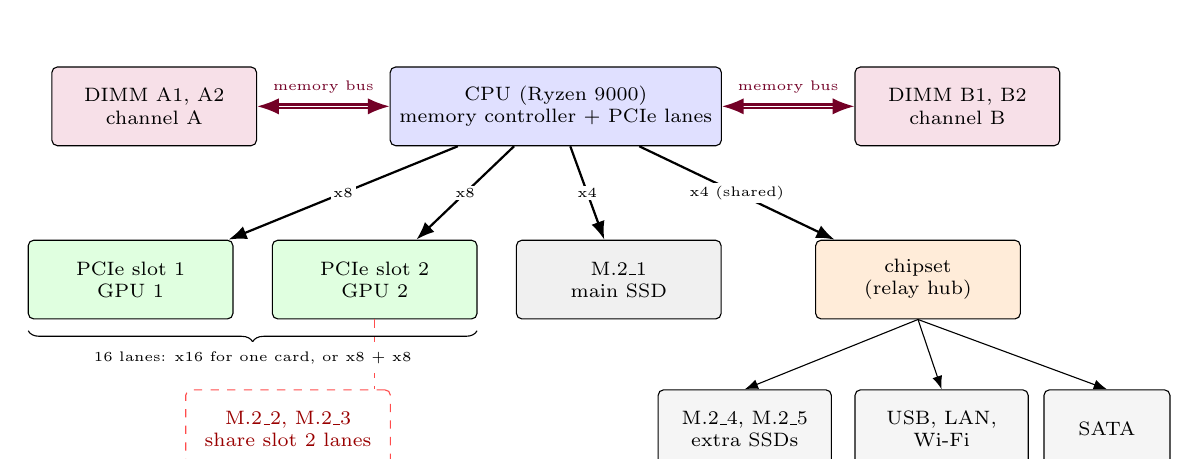
\begin{tikzpicture}[>=Latex,
  box/.style={draw,rounded corners=2pt,minimum width=26mm,minimum height=10mm,font=\scriptsize,align=center},
  lab/.style={font=\tiny,fill=white,inner sep=1pt}]
\node[box,fill=blue!12,minimum width=40mm] (cpu) at (0,0) {CPU (Ryzen 9000)\\memory controller + PCIe lanes};
\node[box,fill=purple!12] (da) at (-5.1,0) {DIMM A1, A2\\channel A};
\node[box,fill=purple!12] (db) at (5.1,0) {DIMM B1, B2\\channel B};
\draw[<->,purple!60!black,double,thick] (da) -- node[above=1pt,font=\tiny] {memory bus} (cpu);
\draw[<->,purple!60!black,double,thick] (db) -- node[above=1pt,font=\tiny] {memory bus} (cpu);
\node[box,fill=green!12] (s1) at (-5.4,-2.2) {PCIe slot 1\\GPU 1};
\node[box,fill=green!12] (s2) at (-2.3,-2.2) {PCIe slot 2\\GPU 2};
\node[box,fill=black!6] (m1) at (0.8,-2.2) {M.2\_1\\main SSD};
\node[box,fill=orange!15] (cs) at (4.6,-2.2) {chipset\\(relay hub)};
\draw[->,thick] (cpu) -- node[lab] {x8} (s1);
\draw[->,thick] (cpu) -- node[lab] {x8} (s2);
\draw[->,thick] (cpu) -- node[lab] {x4} (m1);
\draw[->,thick] (cpu) -- node[lab] {x4 (shared)} (cs);
\node[box,draw=red!70,dashed,text=red!60!black] (m23) at (-3.4,-4.1) {M.2\_2, M.2\_3\\share slot 2 lanes};
\draw[red!70,dashed] (s2.south) -- (m23.north -| s2.south);
\node[box,fill=black!4,minimum width=22mm] (c1) at (2.4,-4.1) {M.2\_4, M.2\_5\\extra SSDs};
\node[box,fill=black!4,minimum width=22mm] (c2) at (4.9,-4.1) {USB, LAN,\\Wi-Fi};
\node[box,fill=black!4,minimum width=16mm] (c3) at (7.0,-4.1) {SATA};
\foreach \c in {c1,c2,c3} \draw[->] (cs.south) -- (\c.north);
\draw[decorate,decoration={brace,amplitude=4pt,mirror}] (-6.7,-2.85) -- (-1.0,-2.85)
  node[midway,below=4pt,font=\tiny,fill=white] {16 lanes: x16 for one card, or x8 + x8};
\end{tikzpicture}

\small CPU에 연결되는 통로 (ASUS X870E 계열 메인보드와 Ryzen 9000의 예). 메모리는 PCIe가 아닌 전용 통로 (보라색 이중선, 메모리 버스)로 연결된다.
검은 화살표는 PCIe lane이다. 그래픽카드 한 장이면 x16, 두 장이면 x8 + x8로 나뉜다.
\end{minipage}
\end{center}

\begin{itemize}[leftmargin=1.5em]
\item \textbf{CPU 직결}: 슬롯이 CPU에 바로 연결된다. 가장 빠르고 다른 장치와 나누지 않는다.
\item \textbf{칩셋 경유}: 칩셋을 거친다. 혼자 쓸 때는 충분하지만, 여러 장치가 동시에 많이 보내면 막힌다.
보급형 메인보드의 두 번째 그래픽카드 슬롯은 흔히 칩셋 경유 x4이다. GPU를 두 장 쓸 계획이면 반드시 확인해야 한다.
\item \textbf{대역 공유} (lane sharing): 두 장치가 같은 lane을 나누어 쓰는 것이다. 위 그림에서 M.2\_2에 SSD를 꽂으면 슬롯 2의 lane을 빼앗아 GPU 2가 꺼진다.
어느 슬롯끼리 나누는지는 메인보드 설명서의 표에 있다.
\item \textbf{메인보드 이름의 B850, X870E} 등은 칩셋의 이름이다. 상위 칩셋일수록 연결할 수 있는 장치가 많다.
\end{itemize}

\paragraph{메모리는 PCIe로 연결하지 않는다.}
CPU 안에는 \textbf{메모리 컨트롤러} (IMC, integrated memory controller)가 있고, 메모리 슬롯은 CPU 소켓의 전용 핀과 배선으로 바로 이어진다.
PCIe lane과는 완전히 별개의 핀과 배선이다.

\begin{itemize}[leftmargin=1.5em]
\item \textbf{버스} (bus): 여러 부품이 데이터를 주고받는 \textbf{공용 전선 묶음}이다.
라틴어 omnibus (``모두를 위한'')에서 온 말로, 여러 사람이 함께 타는 버스처럼 여러 신호선과 장치가 한 통로를 함께 쓴다는 뜻이다.
\textbf{메모리 버스}는 CPU와 메모리 사이의 버스로, 데이터를 나르는 선, 주소와 명령을 나르는 선, 박자를 맞추는 클럭 선으로 이루어진다.
\item \textbf{채널} (channel): 메모리 컨트롤러가 독립적으로 다루는 메모리 버스 하나이다. 채널 하나의 데이터 폭은 $64$비트이다 (DDR5는 이것을 $32$비트 두 개로 나누어 쓴다).
채널이 많을수록 메모리 대역폭이 커진다. 데스크톱 CPU는 $2$채널 (약 $90$ GB/s, DDR5-5600), 서버 CPU는 $8\sim12$채널이다.
\item \textbf{DIMM} (Dual In-line Memory Module): 메모리 칩 여러 개를 작은 기판에 붙인 막대 모양의 모듈이다 (3.1절의 사진).
기판 양면의 금색 접점이 서로 \textbf{다른 신호}를 나르기 때문에 ``dual''이다. 예전의 SIMM (Single In-line)은 양면 접점이 같은 신호였다.
DDR5 DIMM의 접점은 $288$개이다. 노트북용으로 작게 만든 것은 SO-DIMM (small outline DIMM)이다.
\end{itemize}

\begin{center}
\begin{minipage}{\textwidth}\centering
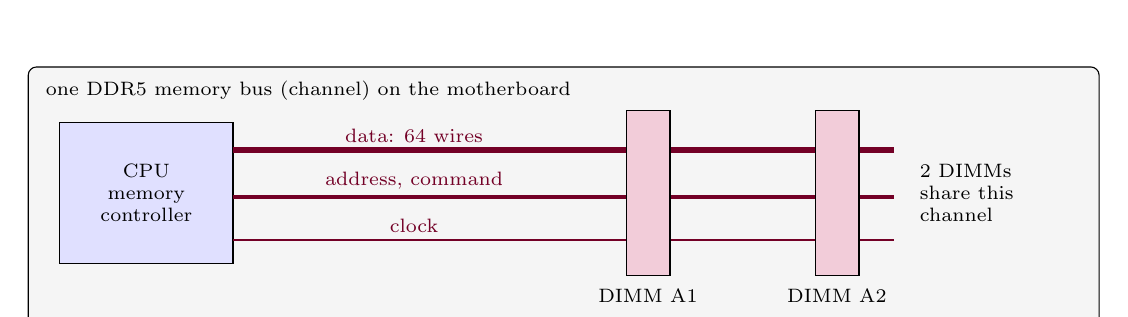
\begin{tikzpicture}[>=Latex,font=\scriptsize]
\draw[fill=black!4,rounded corners=3pt] (0,-0.3) rectangle (13.6,3.0);
\node[anchor=north west] at (0.1,2.95) {one DDR5 memory bus (channel) on the motherboard};
\draw[fill=blue!12] (0.4,0.5) rectangle (2.6,2.3) node[pos=0.5,align=center] {CPU\\memory\\controller};
\foreach \y/\w/\name in {1.95/2.2/{data: 64 wires},1.35/1.4/{address, command},0.8/0.7/{clock}} {
  \draw[purple!60!black,line width=\w pt] (2.6,\y) -- (11.0,\y);
  \node[anchor=south,purple!60!black,inner sep=1pt] at (4.9,\y+0.05) {\name};
}
\foreach \x/\name in {7.6/DIMM A1,10.0/DIMM A2} {
  \draw[fill=purple!20] (\x,0.35) rectangle (\x+0.55,2.45);
  \node[anchor=north] at (\x+0.27,0.3) {\name};
}
\node[align=left,anchor=west] at (11.2,1.4) {2 DIMMs\\share this\\channel};
\end{tikzpicture}

\small 메모리 버스 하나 (한 채널). 전선 묶음이 CPU에서 메모리 슬롯까지 이어지고, 슬롯 두 개가 같은 전선에 매달린다.
\end{minipage}
\end{center}

메인보드의 메모리 슬롯은 $4$개지만 Ryzen 9000의 채널은 $2$개여서, \textbf{채널 하나에 슬롯 두 개}가 매달린다.
그래서 모듈을 $4$장 꽂으면 같은 전선에 모듈 두 개가 달려 전기적 부담이 커지고, 보장 속도가 DDR5-5600에서 DDR5-3600으로 내려간다.
같은 $128$ GB라도 $32$ GB $\times4$보다 $64$ GB $\times2$가 빠른 이유이다 (10절).
메모리는 CPU가 계산하는 내내 읽고 쓰는 곳이어서 지연시간이 매우 중요하다.
그래서 데이터를 패킷으로 포장하는 PCIe 대신, CPU 바로 옆까지 짧게 깐 전용 병렬 버스를 쓴다.

\begin{center}
{\small
\begin{tabular}{@{}lll@{}}
\toprule
& PCIe & 메모리 버스 (DDR5) \\
\midrule
전송 방식 & 직렬 (serial), 데이터를 패킷으로 포장 & 병렬 (parallel), 클럭에 맞추어 바로 전송 \\
폭 & lane 단위 (x1$\sim$x16) & 채널당 $64$비트 \\
거리 & 길어도 된다 (슬롯, 케이블) & 매우 짧아야 한다 \\
연결 대상 & GPU, SSD, 칩셋 등 여러 장치 & 메모리만 \\
장점 & 범용성, 확장성 & 짧은 지연시간 (약 $100$ ns) \\
\bottomrule
\end{tabular}}
\end{center}

\begin{remarkbox}[덧붙임]
\begin{itemize}[leftmargin=1.5em]
\item 예전에는 메모리 컨트롤러가 CPU 밖, 메인보드의 칩 (northbridge)에 있었다. AMD는 2003년, Intel은 2008년쯤부터 CPU 안으로 옮겨 지연시간을 크게 줄였다.
\item GPU도 같다. GPU 칩 안의 메모리 컨트롤러가 VRAM (GDDR, HBM)과 전용 배선으로 바로 이어진다 (\ref{sec:ddr}절). PCIe는 GPU와 CPU 사이에만 쓰인다.
\item 반대 방향의 새 흐름도 있다. \textbf{CXL} (Compute Express Link)은 PCIe와 같은 선로로 메모리를 연결하는 규격으로, 서버에서 메모리를 더 붙이는 데 쓰이기 시작했다.
\end{itemize}
\end{remarkbox}

\subsection{저장장치: HDD, SSD, SATA, NVMe}\label{sec:m2}

데이터셋과 체크포인트는 \textbf{저장장치} (storage)에 둔다.
RAM은 전원이 꺼지면 내용이 사라지는 \textbf{휘발성} (volatile) 메모리이고, 저장장치는 전원이 꺼져도 내용이 남는 \textbf{비휘발성} (non-volatile)이다.
저장장치는 크게 두 종류이다.

\begin{center}
\photo{hdd_35inch_open.jpg}{0.3\textwidth}{3.5인치 하드디스크 (덮개를 연 모습). 원판과 헤드가 달린 팔이 보인다.}\hfill
\photo{ssd_sata_25inch.png}{0.3\textwidth}{2.5인치 SATA SSD (Samsung 870 QVO)}\hfill
\photo{ssd_m2_nvme.jpg}{0.3\textwidth}{M.2 NVMe SSD (Samsung 980 PRO, 2280)}
\end{center}

\paragraph{HDD (Hard Disk Drive).}
자성 물질을 입힌 단단한 원판 (platter)이 분당 $5{,}400\sim7{,}200$번 돌고, 팔 (arm) 끝의 \textbf{헤드}가 원판 위에 아주 가깝게 떠서 자기 신호를 읽고 쓴다.
원하는 데이터를 읽으려면 (1) 팔을 움직여 헤드를 그 트랙으로 옮기고 (\textbf{seek}, 약 $4\sim10$ ms),
(2) 원판이 돌아 그 위치가 헤드 아래로 올 때까지 기다려야 한다 (7,200 rpm이면 평균 반 바퀴 $\approx4.2$ ms).
그래서 \textbf{이어진 데이터}는 초당 약 $200\sim280$ MB로 읽지만, \textbf{여기저기 흩어진 작은 데이터}는 초당 $100\sim200$번밖에 읽지 못한다.
대신 용량당 가격이 싸서 (한 대에 수십 TB) 보관용으로 쓴다.

\paragraph{SSD (Solid State Drive).}
움직이는 부품 없이 \textbf{NAND flash}라는 반도체에 저장한다. ``solid state''는 움직이는 기계 부품이 없는 전자 장치라는 뜻이다.
flash의 셀 (cell) 하나는 전하를 가두어 두는 트랜지스터이고, 갇힌 전하의 양으로 비트를 나타낸다. 전하는 전원이 꺼져도 갇혀 있으므로 비휘발성이다.
SSD 안의 \textbf{컨트롤러}는 여러 NAND 칩에 여러 채널로 \textbf{동시에} 접근한다. 작은 GPU처럼 병렬로 일하는 셈이다.
그래서 임의 위치를 읽는 데 약 $0.05\sim0.1$ ms이고, 초당 수십만$\sim$백만 번 읽는다.

\begin{center}
\begin{minipage}{\textwidth}\centering
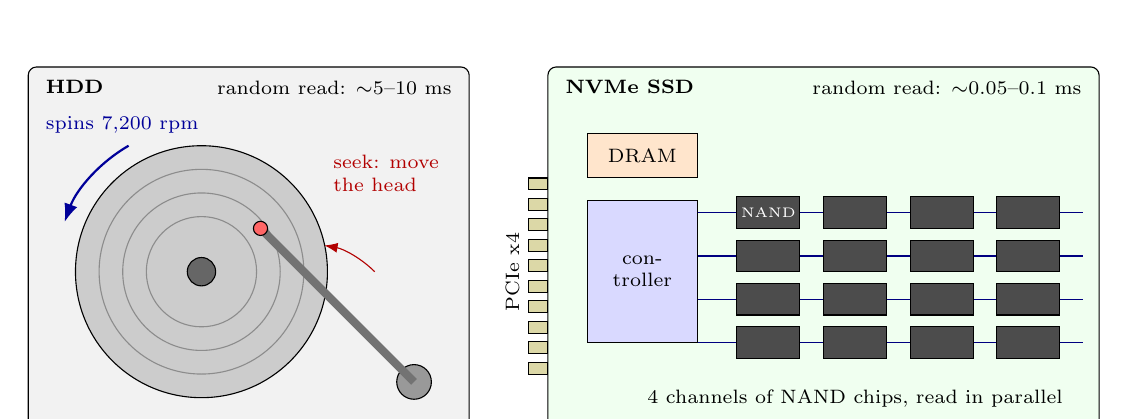
\begin{tikzpicture}[font=\scriptsize,>=Latex]
% ---- HDD ----
\begin{scope}
\draw[fill=black!5,rounded corners=3pt] (0,0) rectangle (5.6,4.6);
\node[anchor=north west] at (0.1,4.55) {\textbf{HDD}};
\node[anchor=north east] at (5.5,4.55) {random read: $\sim$5--10 ms};
\draw[fill=black!20] (2.2,2.0) circle (1.6);
\foreach \r in {0.7,1.0,1.3} \draw[black!45] (2.2,2.0) circle (\r);
\draw[fill=black!60] (2.2,2.0) circle (0.18);
\draw[->,thick,blue!60!black] (1.275,3.6) arc (120:160:1.85);
\node[blue!60!black,anchor=north west] at (0.1,4.1) {spins 7,200 rpm};
\draw[fill=black!40] (4.9,0.6) circle (0.22);
\draw[line width=3pt,black!55] (4.9,0.6) -- (2.95,2.55);
\draw[fill=red!60] (2.95,2.55) circle (0.09);
\draw[->,red!70!black] (4.4,2.0) arc (45:80:1.2);
\node[red!70!black,anchor=west,align=left] at (3.75,3.25) {seek: move\\the head};
\end{scope}
% ---- SSD ----
\begin{scope}[xshift=6.6cm]
\draw[fill=green!6,rounded corners=3pt] (0,0) rectangle (7.0,4.6);
\node[anchor=north west] at (0.1,4.55) {\textbf{NVMe SSD}};
\node[anchor=north east] at (6.9,4.55) {random read: $\sim$0.05--0.1 ms};
\foreach \k in {0,...,9} \draw[fill=yellow!60!black!40] (-0.25,0.7+\k*0.26) rectangle (0,0.85+\k*0.26);
\node[rotate=90] at (-0.45,2.0) {PCIe x4};
\draw[fill=blue!15] (0.5,1.1) rectangle (1.9,2.9) node[pos=0.5,align=center] {con-\\troller};
\draw[fill=orange!20] (0.5,3.2) rectangle (1.9,3.75) node[pos=0.5] {DRAM};
\foreach \c in {0,...,3} {
  \pgfmathsetmacro{\y}{2.75-\c*0.55}
  \draw[blue!50!black] (1.9,\y) -- (6.8,\y);
  \foreach \n in {0,...,3} \draw[fill=black!70] (2.4+\n*1.1,\y-0.2) rectangle ++(0.8,0.4);
}
\node[white,font=\tiny] at (2.8,2.75) {NAND};
\node[anchor=south] at (3.9,0.15) {4 channels of NAND chips, read in parallel};
\end{scope}
\end{tikzpicture}

\small HDD와 SSD의 구조. HDD는 헤드를 옮기고 원판이 돌기를 기다려야 하고, SSD는 컨트롤러가 여러 NAND 칩을 동시에 읽는다.
\end{minipage}
\end{center}

\paragraph{셀 하나에 몇 비트?}
NAND flash는 셀 하나에 갇힌 전하의 양을 여러 단계로 나누어 \textbf{셀 하나에 여러 비트}를 저장한다.
$n$비트를 저장하려면 전하를 $2^n$단계로 구별해야 한다.

\begin{center}
\begin{minipage}{\textwidth}\centering
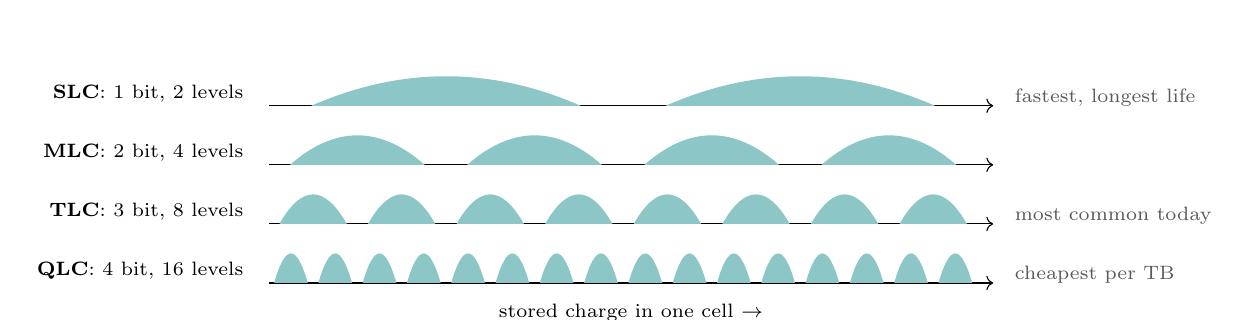
\begin{tikzpicture}[font=\scriptsize,x=1cm,y=1cm]
\foreach \row/\name/\n/\use in {0/SLC/1/{fastest, longest life}, 1/MLC/2/{}, 2/TLC/3/{most common today}, 3/QLC/4/{cheapest per TB}} {
  \pgfmathsetmacro{\y}{-\row*0.75}
  \pgfmathtruncatemacro{\L}{2^\n}
  \node[anchor=east] at (-0.2,\y+0.15) {\textbf{\name}: \n\ bit, \L\ levels};
  \draw[->] (0,\y) -- (9.2,\y);
  \foreach \i in {1,...,\L} {
    \pgfmathsetmacro{\cx}{(\i-0.5)*9/\L}
    \pgfmathsetmacro{\hw}{0.38*9/\L}
    \fill[teal!45] (\cx-\hw,\y) .. controls (\cx-\hw/3,\y+0.5) and (\cx+\hw/3,\y+0.5) .. (\cx+\hw,\y) -- cycle;
  }
  \node[anchor=west,black!65] at (9.35,\y+0.1) {\use};
}
\node[anchor=north] at (4.6,-2.4) {stored charge in one cell $\rightarrow$};
\end{tikzpicture}

\small 셀 하나에 저장하는 비트 수. 비트가 늘수록 구별할 전하 단계가 $2$배씩 늘어나 단계 사이의 간격이 좁아진다.
\end{minipage}
\end{center}

\begin{center}
{\small
\begin{tabular}{@{}llc>{\raggedright\arraybackslash}p{66mm}@{}}
\toprule
종류 & 셀 하나의 비트 & 전하 단계 & 특징 \\
\midrule
SLC (Single-Level Cell) & $1$ & $2$ & 가장 빠르고 수명이 길다. 비싸다 \\
MLC (Multi-Level Cell) & $2$ & $4$ & \\
TLC (Triple-Level Cell) & $3$ & $8$ & 지금 가장 흔하다 (사진의 980 PRO) \\
QLC (Quad-Level Cell) & $4$ & $16$ & 가장 싸고 크다. 쓰기가 느리고 수명이 짧다 (사진의 870 QVO) \\
\bottomrule
\end{tabular}}
\end{center}

비트를 많이 넣을수록 같은 칩에 더 많이 저장하지만, 단계 사이의 간격이 좁아져 쓰기가 느려지고 셀이 견디는 쓰기 횟수가 줄어든다.
SSD의 수명은 \textbf{TBW} (TeraBytes Written, 평생 쓸 수 있는 양)로 표시한다. 체크포인트를 아주 자주 덮어쓰는 학습에서는 한 번쯤 확인할 만하다.

\begin{remarkbox}[NAND와 flash라는 이름]
\textbf{NAND}는 디지털 논리 회로의 기본 게이트 NOT AND의 이름이다. NAND flash는 셀 (트랜지스터) 수십 개를 \textbf{한 줄로 직렬로} 이어 쓰는데,
이 모양이 NAND 게이트의 회로와 닮아서 붙은 이름이다. 셀마다 따로 연결하는 \textbf{NOR flash}는 그 모양이 NOR (NOT OR) 게이트와 닮았다.

\begin{center}
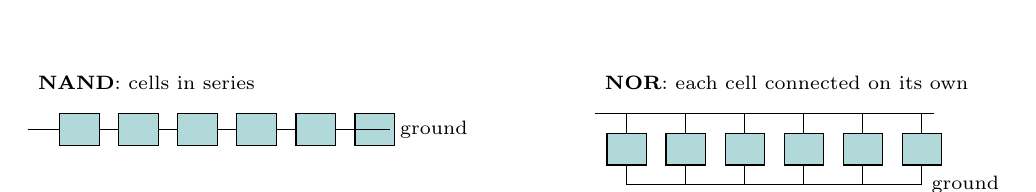
\begin{tikzpicture}[font=\scriptsize]
\begin{scope}
\node[anchor=west] at (0,1.0) {\textbf{NAND}: cells in series};
\draw (0,0.4) -- (0.4,0.4);
\foreach \i in {0,...,5} \draw[fill=teal!30] (0.4+\i*0.75,0.2) rectangle ++(0.5,0.4);
\foreach \i in {0,...,4} \draw (0.9+\i*0.75,0.4) -- (1.15+\i*0.75,0.4);
\draw (4.15,0.4) -- (4.6,0.4) node[right] {ground};
\end{scope}
\begin{scope}[xshift=7.2cm]
\node[anchor=west] at (0,1.0) {\textbf{NOR}: each cell connected on its own};
\draw (0,0.6) -- (4.3,0.6);
\foreach \i in {0,...,5} {
  \draw (0.4+\i*0.75,0.6) -- (0.4+\i*0.75,0.35);
  \draw[fill=teal!30] (0.15+\i*0.75,-0.05) rectangle ++(0.5,0.4);
  \draw (0.4+\i*0.75,-0.05) -- (0.4+\i*0.75,-0.3);
}
\draw (0.4,-0.3) -- (4.15,-0.3) node[right] {ground};
\end{scope}
\end{tikzpicture}
\end{center}

\begin{center}
{\small
\begin{tabular}{@{}lll@{}}
\toprule
& NAND flash & NOR flash \\
\midrule
연결 & 셀을 직렬로 이음 & 셀마다 따로 연결 \\
집적도 & 배선과 접점이 적어 촘촘하고 싸다 & 배선이 많아 덜 촘촘하다 \\
읽기 & 페이지 (수 KB) 단위 & 바이트 하나도 바로 \\
쓰는 곳 & SSD, USB 메모리, 휴대폰 저장공간 & 메인보드의 BIOS 칩 등 작은 펌웨어 \\
\bottomrule
\end{tabular}}
\end{center}

\textbf{flash}는 1980년대 도시바의 마스오카 후지오 (Fujio Masuoka)가 발명한 메모리의 이름이다 (NOR 1984년, NAND 1987년).
그 전의 비휘발성 메모리 (EEPROM)는 바이트 단위로 하나씩 지웠는데, 이 메모리는 큰 덩어리 (block)를 \textbf{한 번에 순식간에} 지웠다.
그 모습이 카메라 플래시가 번쩍 터지는 것 같다고 하여 flash라는 이름이 붙었다고 한다.
요즘은 셀의 줄을 위로 $100$층 넘게 쌓은 \textbf{3D NAND} (삼성은 V-NAND라고 부른다)가 표준이다.

\medskip
\textbf{SSD의 동작과의 관계.} 읽기와 쓰기는 페이지 (수 KB) 단위, 지우기는 블록 (수 MB) 단위이다.
이미 쓴 페이지에 바로 덮어쓸 수 없고 블록을 통째로 지운 뒤에만 다시 쓸 수 있다.
그래서 SSD 컨트롤러는 새 데이터를 빈 페이지에 쓰고, 쓸모없어진 페이지가 많은 블록을 나중에 모아 지운다 (\textbf{garbage collection}).
운영체제의 \textbf{TRIM} 명령은 ``이 데이터는 지워도 된다''고 SSD에 알려 이 정리를 돕는다.
셀은 지우고 쓸 때마다 조금씩 닳으며, 이것이 TBW로 표시하는 수명이다.
\end{remarkbox}

\paragraph{연결 규격: ATA, SATA, NVMe, M.2.}
\begin{itemize}[leftmargin=1.5em]
\item \textbf{ATA} (AT Attachment): 1984년 IBM PC/AT (AT는 Advanced Technology)에 하드디스크를 붙이던 방식에서 온 이름이다.
제어 회로를 드라이브 안에 넣어서 \textbf{IDE} (Integrated Drive Electronics)라고도 불렀다.
넓은 리본 케이블 ($40\sim80$가닥)로 $16$비트를 병렬로 보냈고, 지금은 \textbf{PATA} (Parallel ATA)라고 부른다.
\item \textbf{SATA} (Serial ATA, 2003): 같은 일을 전선 몇 가닥으로 \textbf{직렬} 전송하도록 바꾼 것이다 (\ref{sec:width}절).
최대 $6$ Gbit/s로, 실제로는 약 $0.55$ GB/s이다. 하드디스크의 속도에 맞춘 규격이라 SSD에게는 좁다.
\item \textbf{NVMe} (Non-Volatile Memory Express, 2011): flash용으로 새로 만든 통신 규격이다. SSD를 \textbf{PCIe lane}에 직접 연결하고,
명령을 담는 대기열을 최대 $65{,}536$개까지 두어 여러 CPU 코어가 동시에 요청할 수 있다 (SATA는 대기열 $1$개, 명령 $32$개).
PCIe 4.0 x4이면 약 $7$ GB/s, PCIe 5.0 x4이면 약 $14$ GB/s이다.
\item \textbf{M.2} (``엠닷투''): SSD를 꽂는 작은 슬롯과 기판의 \textbf{모양} 규격이다. 길이는 $2280$ ($22$ mm $\times$ $80$ mm)이 가장 흔하다.
모양의 이름일 뿐이어서 M.2 슬롯에 꽂는 SATA SSD도 있다. 사기 전에 ``NVMe''인지 확인한다.
\end{itemize}

\begin{center}
{\small
\begin{tabular}{@{}lcccl@{}}
\toprule
& 이어서 읽기 & 작은 데이터 임의 읽기 & 한 번의 지연 & 쓰는 곳 \\
\midrule
HDD (7,200 rpm) & $\sim$0.25 GB/s & $\sim$150번/초 & $\sim$5--10 ms & 보관, 백업 \\
SATA SSD & $\sim$0.55 GB/s & $\sim$10만 번/초 & $\sim$0.1 ms & 예전 컴퓨터 \\
NVMe SSD, PCIe 4.0 & $\sim$7 GB/s & $\sim$100만 번/초 & $\sim$0.05 ms & 운영체제, 학습 데이터 \\
NVMe SSD, PCIe 5.0 & $\sim$14 GB/s & $\sim$150만 번/초 & $\sim$0.05 ms & 최신 컴퓨터 \\
\bottomrule
\end{tabular}}

\small 대략적인 값. 작은 데이터 ($4$ KB) 임의 읽기 성능을 \textbf{IOPS} (Input/Output Operations Per Second)라고 한다.
\end{center}

\paragraph{딥러닝에서의 의미.}
이미지 데이터셋은 작은 파일이 매우 많다. 예를 들어 ImageNet의 훈련 데이터는 평균 약 $110$ KB인 이미지 $128$만 장이다.
미니배치를 만들 때마다 \textbf{무작위 순서}로 읽으므로, 이어서 읽기보다 \textbf{임의 읽기} 성능이 중요하다.
HDD에서 초당 $150$장씩 읽으면 한 epoch에 파일 읽기만 $1{,}280{,}000/150\approx8{,}500$초, 약 $2.4$시간이 걸린다. GPU는 그동안 대부분 논다.
NVMe SSD에서는 파일 읽기가 병목이 되지 않고, 이미지를 여는 CPU의 계산 (JPEG 디코딩)이 먼저 병목이 된다.

\begin{itemize}[leftmargin=1.5em]
\item 학습 데이터는 \textbf{NVMe SSD}에 둔다. HDD나 네트워크 저장소 (NAS)는 보관용으로 쓰고, 학습 전에 NVMe로 복사한다.
\item 작은 파일이 아주 많으면 몇 개의 큰 파일로 묶는다 (tar 묶음, HDF5, LMDB, WebDataset 등). 임의 읽기가 이어서 읽기로 바뀐다.
\item 운영체제는 한 번 읽은 파일을 남는 RAM에 보관한다 (page cache). 데이터셋이 RAM보다 작으면 두 번째 epoch부터는 RAM에서 읽는다. RAM을 넉넉히 두는 이유 중 하나이다.
\end{itemize}

\subsection{메인보드에서 찾아보기}\label{sec:board_photo}

\begin{center}
\begin{minipage}{\textwidth}\centering
\begin{tikzpicture}[font=\scriptsize,
  lead/.style={draw=white,line width=2.2pt},
  dot/.style={circle,fill=#1,draw=white,line width=0.8pt,inner sep=1.6pt}]
\node[anchor=south west,inner sep=0] (img) at (0,0)
  {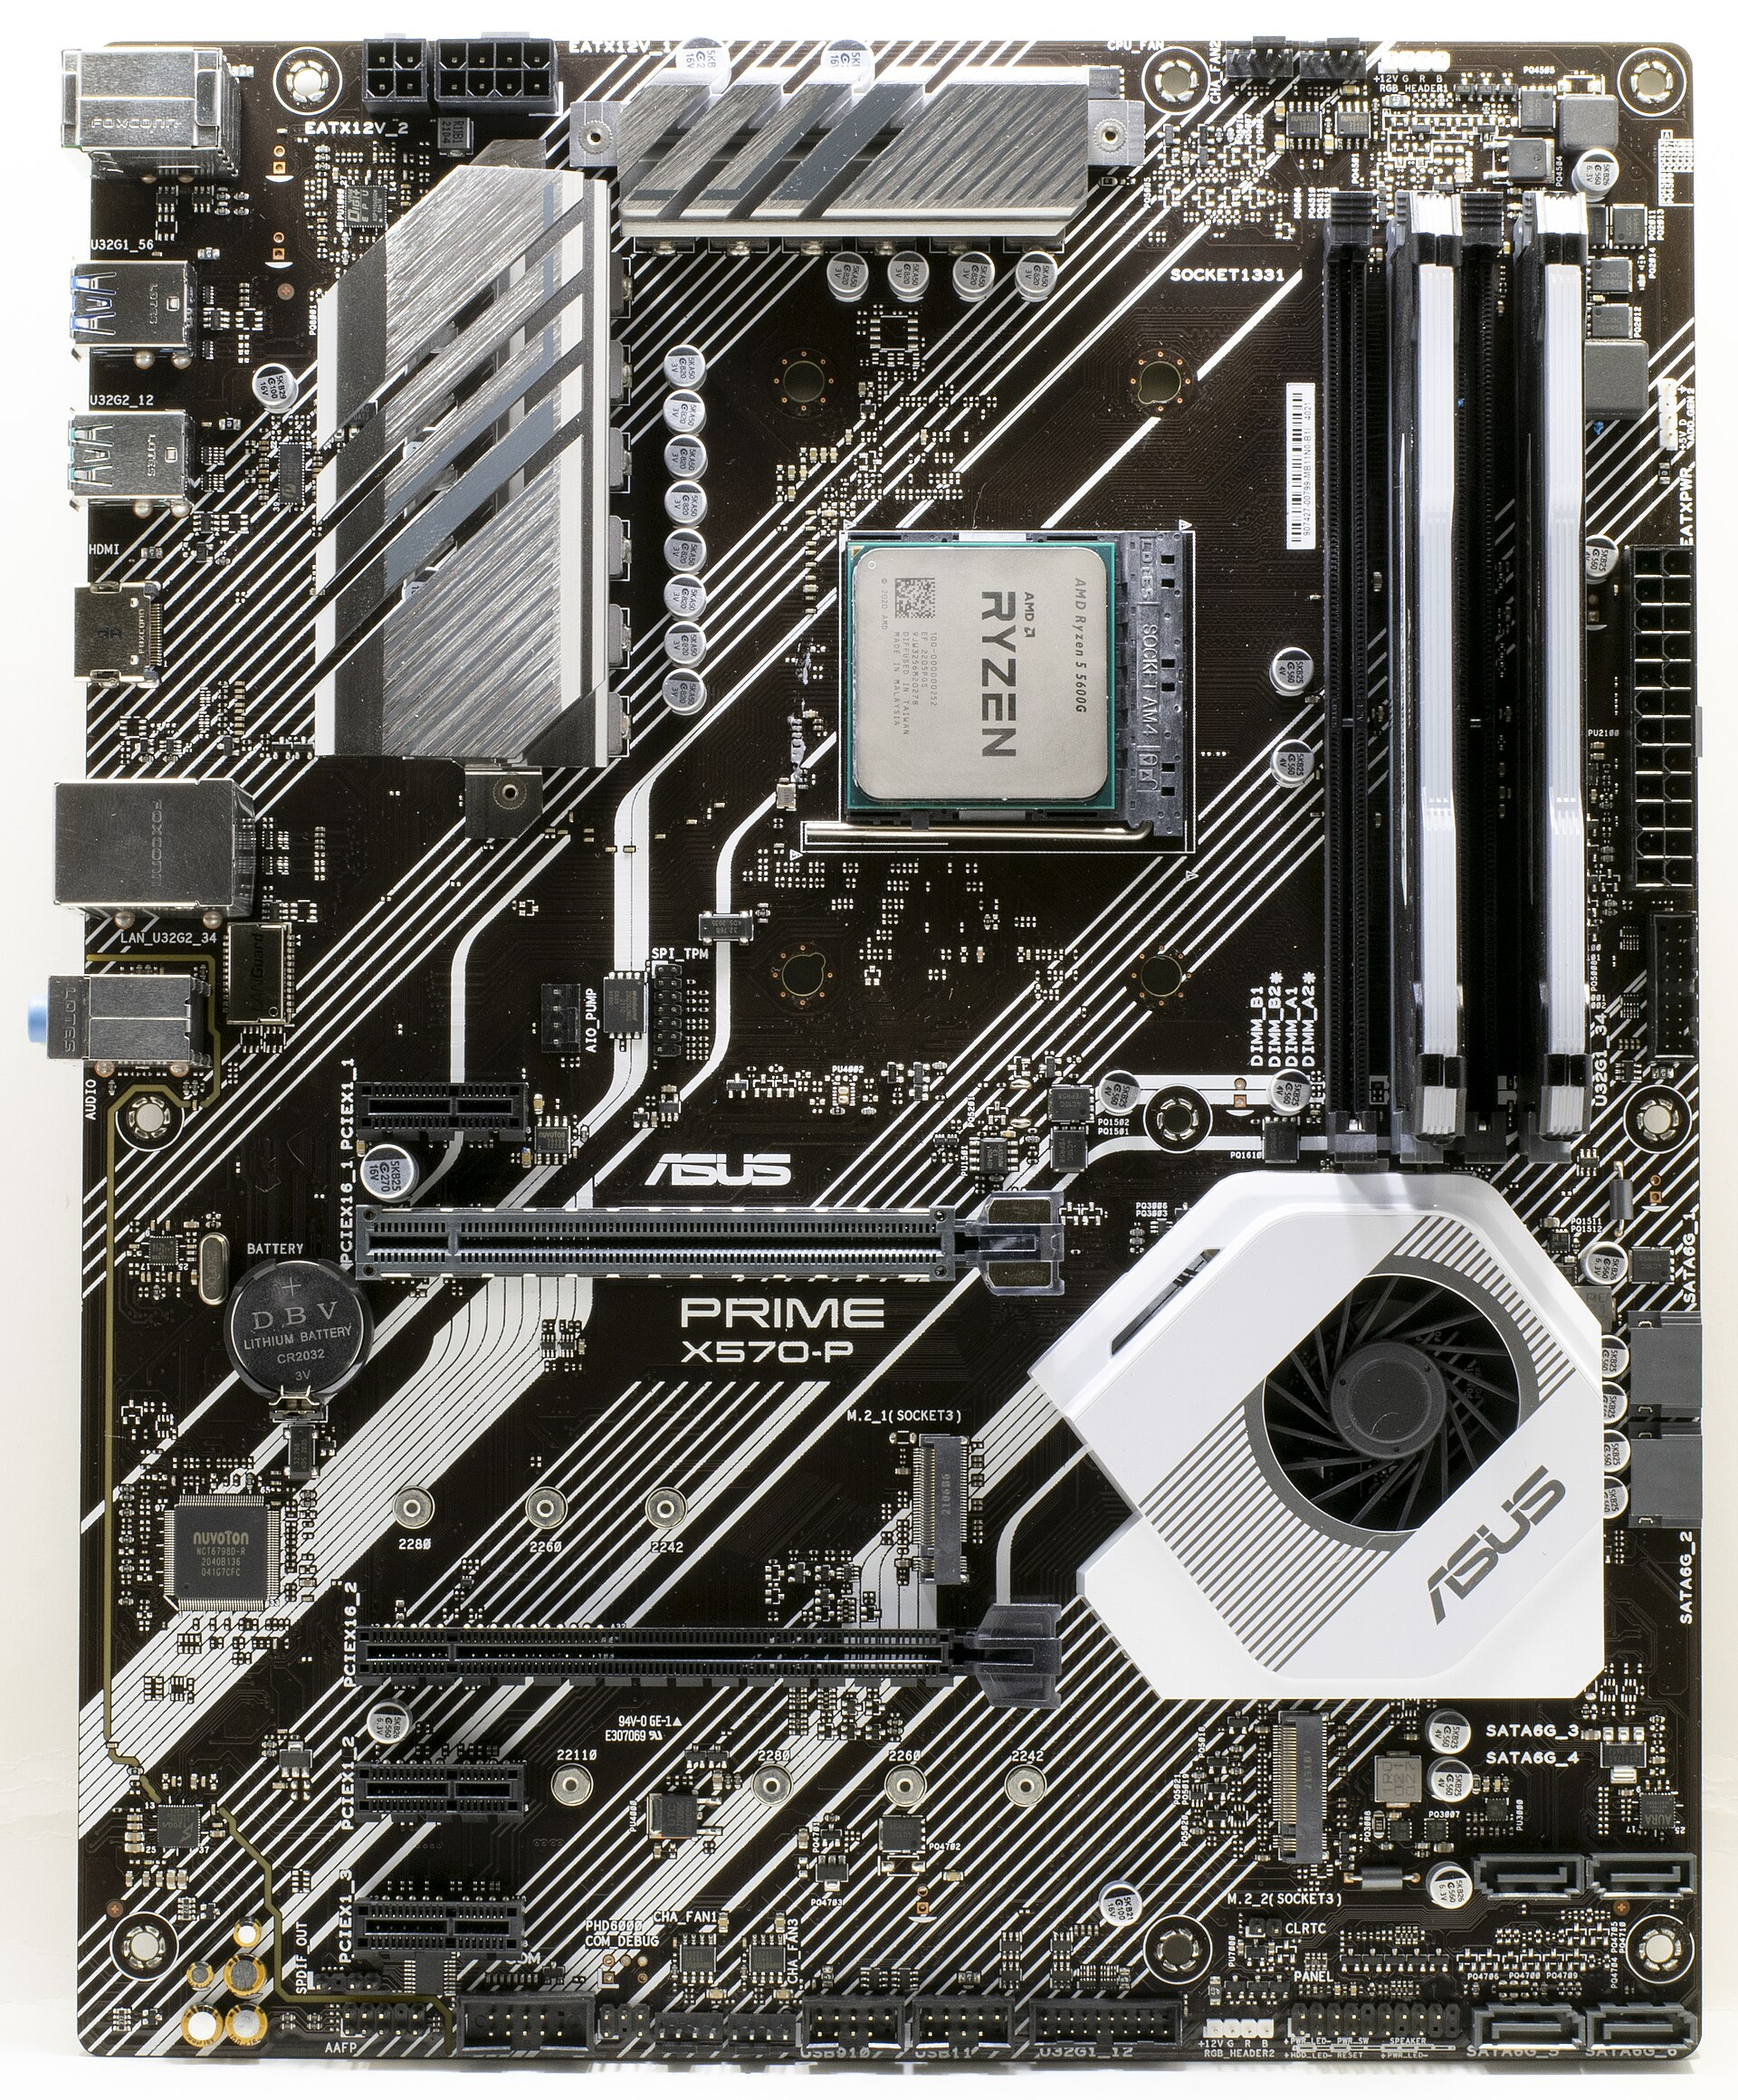
\includegraphics[width=7.0cm]{figures/photos/motherboard_atx_x570_top.jpg}};
\begin{scope}[x={(img.south east)},y={(img.north west)}]
% target point / label height / side / color / text
\foreach \px/\py/\ly/\side/\c/\t in {
  0.284/0.965/0.965/L/black/{CPU power (8-pin)},
  0.079/0.760/0.760/L/black/{rear I/O: USB, LAN, HDMI},
  0.254/0.465/0.500/L/orange!80!black/{PCIEX1\_1: x1, chipset},
  0.375/0.410/0.410/L/blue!60!black/{PCIEX16\_1: x16, CPU (GPU)},
  0.172/0.370/0.320/L/black/{battery (BIOS settings)},
  0.387/0.225/0.225/L/red!70!black/{PCIEX16\_2: x16 size,\\x4 via chipset},
  0.834/0.720/0.810/R/blue!60!black/{DIMM slots (4)},
  0.961/0.655/0.710/R/black/{24-pin ATX power},
  0.562/0.675/0.610/R/blue!60!black/{CPU in its socket (AM4)},
  0.779/0.310/0.420/R/orange!80!black/{chipset X570 (under the fan)},
  0.958/0.270/0.320/R/black/{SATA ports},
  0.541/0.290/0.210/R/blue!60!black/{M.2\_1: SSD, x4, CPU},
  0.749/0.155/0.110/R/orange!80!black/{M.2\_2: SSD, chipset}} {
  \if\side L
    \draw[lead] (\px,\py) -- (-0.03,\ly);
    \draw[\c,thick] (\px,\py) -- (-0.03,\ly);
    \node[anchor=east,text=\c,align=right] at (-0.035,\ly) {\t};
  \else
    \draw[lead] (\px,\py) -- (1.03,\ly);
    \draw[\c,thick] (\px,\py) -- (1.03,\ly);
    \node[anchor=west,text=\c,align=left] at (1.035,\ly) {\t};
  \fi
  \node[dot=\c] at (\px,\py) {};
}
\end{scope}
\end{tikzpicture}

\small 데스크톱 메인보드 (ASUS Prime X570-P)의 주요 부분. 파랑은 CPU에 직접 연결된 부분, 주황은 칩셋에 연결된 부분이다.
두 번째 x16 슬롯은 모양만 x16이고, 실제로는 칩셋을 거친 x4로 동작한다 (빨강). 이런 보드에 GPU 두 장을 꽂으면 두 번째 GPU는 좁은 통로를 쓴다.
\end{minipage}
\end{center}

\begin{center}
\photo{pcie_slots_gigabyte.jpg}{0.45\textwidth}{여러 PCIe 슬롯. 맨 위가 x16, 가운데 짧은 것이 x1이다. 그 아래의 긴 슬롯은 기판에 ``PCIEX4''라고 적혀 있듯이 길이만 x16이고 lane은 $4$개이다. 맨 아래 두 개는 옛 PCI 슬롯이다.}\hfill
\photo{cpu_ryzen_am4_pins.jpg}{0.45\textwidth}{CPU의 아랫면 (AM4). 이 핀들로 전원, 메모리, PCIe lane이 나간다.}
\end{center}

\subsection{PCIe가 학습 속도에 미치는 영향}\label{sec:pcie_matters}

GPU를 x16 대신 x8로 꽂으면 학습이 절반으로 느려질까? 대부분은 \textbf{아니다}.

\begin{itemize}[leftmargin=1.5em]
\item 학습 중 데이터 대부분은 GPU \textbf{안}에서 오간다 (VRAM $\leftrightarrow$ SM). PCIe로는 미니배치만 건너간다.
\item 예를 들어 $224\times224$ 컬러 이미지 $256$장의 미니배치는 \texttt{float32}로 $256\times3\times224\times224\times4\approx154$ MB이다.
PCIe 5.0 x8 ($\sim$32 GB/s)으로 약 $5$ ms이고, 이 미니배치의 계산은 보통 그보다 훨씬 오래 걸린다.
\item PCIe가 중요해지는 것은 \textbf{여러 GPU가 기울기를 주고받을 때}이다 (7.4절). 모델이 크고 GPU 사이에 NVLink가 없으면 PCIe로 주고받는다.
\end{itemize}

\texttt{gpu\_bench.py}로 강의자의 노트북을 재어 보면, CPU 메모리에서 GPU로 보내는 속도가 약 $6.3$ GB/s였다.
\texttt{nvidia-smi}로 확인하면 이 노트북의 GPU는 \textbf{PCIe 4.0 x4}로 연결되어 있다 (이론값 약 $8$ GB/s).
노트북은 배선 공간이 좁아 GPU에 lane을 적게 주는 경우가 많다.

\begin{remarkbox}[pinned memory]
보통의 메모리 (pageable memory)는 운영체제가 언제든 다른 곳으로 옮길 수 있어서, GPU로 보낼 때 한 번 더 복사를 거친다.
\textbf{pinned memory} (page-locked memory)는 고정된 메모리여서 GPU가 직접 읽어 간다.
\texttt{DataLoader(..., pin\_memory=True)}로 켤 수 있고, 복사를 계산과 겹쳐서 할 수 있게 된다 (\texttt{.to(device, non\_blocking=True)}).
\end{remarkbox}

% =================================================
\section{메모리}\label{sec:memory}
% =================================================

\subsection{RAM, DRAM, SRAM}\label{sec:ram}

\begin{itemize}[leftmargin=1.5em]
\item \textbf{RAM} (Random Access Memory, 임의 접근 메모리): 주소만 알면 \textbf{어느 위치든} 거의 같은 시간에 읽고 쓸 수 있는 메모리이다.
옛날의 자기 테이프는 원하는 위치까지 차례로 감아야 했다 (sequential access). 그와 대비한 이름이다.
\item \textbf{DRAM} (Dynamic RAM): 비트 하나를 작은 \textbf{축전기 (커패시터)의 전하}로 저장한다. 전하가 조금씩 새기 때문에 수십 ms마다 읽어서 다시 써야 (refresh) 한다.
가만히 두면 사라진다는 뜻에서 ``동적 (dynamic)''이다. 칸 하나가 트랜지스터 $1$개와 축전기 $1$개로 작아서, 싸고 크게 만들 수 있다.
1966년 IBM의 Robert Dennard가 발명하였다.
\item \textbf{SRAM} (Static RAM): 트랜지스터 $6$개로 된 회로에 저장하여 refresh가 필요 없다. 빠르지만 크고 비싸다. CPU와 GPU 안의 \textbf{캐시}(cache)에 쓴다.
\end{itemize}

이 자료에 나오는 DDR5, GDDR7, HBM3e는 \textbf{모두 DRAM}이다. 저장하는 칸은 같고, 칩을 배치하고 프로세서에 연결하는 방법이 다르다.

\begin{center}
\photo{dram_chips_ddr4_module.png}{0.8\textwidth}{방열판이 없는 메모리 모듈 (DDR4). 검은 사각형 하나하나가 DRAM 칩이다.}
\end{center}

\subsection{D램과 낸드: 메모리 반도체의 두 종류}\label{sec:dram_nand}

뉴스에서 말하는 \textbf{메모리 반도체}는 대부분 \textbf{D램} (DRAM)과 \textbf{낸드} (NAND flash) 두 가지이다.
둘 다 비트를 \textbf{전하}로 저장하지만, 전하를 담는 방법이 달라서 성질이 거의 정반대이다.
이 자료에서 DDR5, GDDR7, HBM3e는 모두 D램이고, SSD 안의 저장 칩은 낸드이다.

\paragraph{D램의 셀: 트랜지스터 1개와 커패시터 1개.}
D램의 칸 (셀) 하나는 스위치 역할을 하는 \textbf{트랜지스터}와, 전하를 담는 아주 작은 \textbf{커패시터} (축전기)로 되어 있다 (1T1C).
커패시터에 전하가 차 있으면 $1$, 비어 있으면 $0$이다.
셀은 가로줄 (\textbf{word line}, 행을 고르는 선)과 세로줄 (\textbf{bit line}, 데이터가 오가는 선)이 만나는 곳마다 하나씩 있다.

\begin{center}
\begin{minipage}{\textwidth}\centering
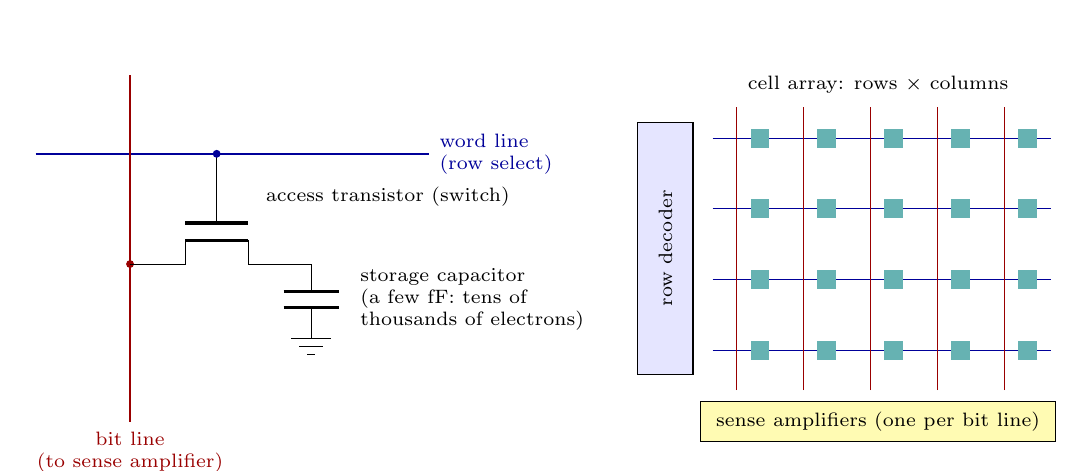
\begin{tikzpicture}[font=\scriptsize,>=Latex]
% ---- one DRAM cell ----
\begin{scope}
\draw[thick,blue!60!black] (-0.6,3.0) -- (4.4,3.0) node[right,align=left] {word line\\(row select)};
\draw[thick,red!60!black] (0.6,4.0) -- (0.6,-0.4) node[below,align=center] {bit line\\(to sense amplifier)};
\fill[red!60!black] (0.6,1.6) circle (0.05);
% access transistor (MOSFET): channel between the bit line and the capacitor, gate on the word line
\draw (0.6,1.6) -- (1.3,1.6) -- (1.3,1.9);
\draw[very thick] (1.3,1.9) -- (2.1,1.9);
\draw (2.1,1.9) -- (2.1,1.6) -- (2.9,1.6);
\draw[very thick] (1.3,2.12) -- (2.1,2.12);
\draw (1.7,2.12) -- (1.7,3.0);
\fill[blue!60!black] (1.7,3.0) circle (0.05);
\node[anchor=west,align=left] at (2.2,2.45) {access transistor (switch)};
% storage capacitor to ground
\draw (2.9,1.6) -- (2.9,1.25);
\draw[very thick] (2.55,1.25) -- (3.25,1.25);
\draw[very thick] (2.55,1.05) -- (3.25,1.05);
\draw (2.9,1.05) -- (2.9,0.65);
\draw (2.65,0.65) -- (3.15,0.65);
\draw (2.75,0.55) -- (3.05,0.55);
\draw (2.85,0.45) -- (2.95,0.45);
\node[anchor=west,align=left] at (3.4,1.15) {storage capacitor\\(a few fF: tens of\\thousands of electrons)};
\end{scope}
% ---- array ----
\begin{scope}[xshift=8.3cm,yshift=0.1cm]
\foreach \r in {0,...,3} \draw[blue!60!black] (-0.3,\r*0.9+0.4) -- (4.0,\r*0.9+0.4);
\foreach \c in {0,...,4} \draw[red!60!black] (\c*0.85,-0.1) -- (\c*0.85,3.5);
\foreach \r in {0,...,3} \foreach \c in {0,...,4} \fill[teal!60] (\c*0.85+0.18,\r*0.9+0.4-0.12) rectangle ++(0.24,0.24);
\draw[fill=yellow!30] (-0.45,-0.75) rectangle (4.05,-0.25) node[pos=0.5] {sense amplifiers (one per bit line)};
\draw[fill=blue!10] (-1.25,0.1) rectangle (-0.55,3.3) node[pos=0.5,rotate=90] {row decoder};
\node[anchor=south] at (1.8,3.55) {cell array: rows $\times$ columns};
\end{scope}
\end{tikzpicture}

\small 왼쪽: D램 셀 하나 (트랜지스터 $1$개 $+$ 커패시터 $1$개). 오른쪽: 셀들이 행과 열로 놓인 배열. 행 하나를 고르면 그 행의 모든 셀이 동시에 bit line에 연결된다.
\end{minipage}
\end{center}

\begin{itemize}[leftmargin=1.5em]
\item \textbf{쓰기}: word line에 전압을 주어 트랜지스터를 열고, bit line의 전압으로 커패시터를 채우거나 비운다.
\item \textbf{읽기}: 행 하나를 열면 그 행의 커패시터들이 각자의 bit line과 연결되어, bit line의 전압이 \textbf{아주 조금} 오르거나 내린다.
커패시터가 bit line보다 훨씬 작아서 변화가 작으므로, bit line마다 달린 \textbf{감지 증폭기} (sense amplifier)가 그 차이를 키워 $0$과 $1$을 가린다.
이때 커패시터의 전하가 빠져나가므로, 읽은 값을 곧바로 \textbf{다시 써 넣는다} (파괴적 읽기, destructive read).
\item \textbf{refresh}: 커패시터의 전하는 가만히 두어도 조금씩 샌다.
그래서 메모리 컨트롤러는 정해진 시간 안에 모든 행을 한 번씩 읽고 다시 쓴다 (JEDEC 규격에서 DDR4는 $64$ ms, DDR5는 $32$ ms).
전원이 꺼지면 refresh도 멈추므로 내용이 사라진다. 이것이 D램이 \textbf{휘발성}인 이유이다.
\end{itemize}

칩 안에서 행 하나 (수 KB)를 여는 데는 시간이 걸리지만, 이미 열린 행에서 이웃한 열을 연달아 읽는 것은 빠르다.
\ref{sec:bandwidth}절에서 볼 ``연속된 주소를 덩어리로 읽을 때 가장 빠르다''는 성질이 여기에서 나온다.
칩 하나에는 이런 배열 (bank)이 여러 개 있어서 서로 다른 bank를 번갈아 열며 기다리는 시간을 숨긴다.

\paragraph{낸드의 셀: 전하를 가두는 트랜지스터.}
낸드의 셀은 커패시터가 없다. 트랜지스터 자체의 게이트 아래에 \textbf{절연막으로 둘러싸인 층}을 하나 더 두고, 그 층에 전자를 가둔다.
갇힌 전자는 트랜지스터가 켜지는 데 필요한 전압 (문턱전압, threshold voltage)을 높인다.
그래서 읽을 때는 게이트에 정해진 전압을 걸어 트랜지스터가 켜지는지를 본다. 켜지면 전자가 적은 것이고, 안 켜지면 많은 것이다.

\begin{center}
\begin{minipage}{\textwidth}\centering
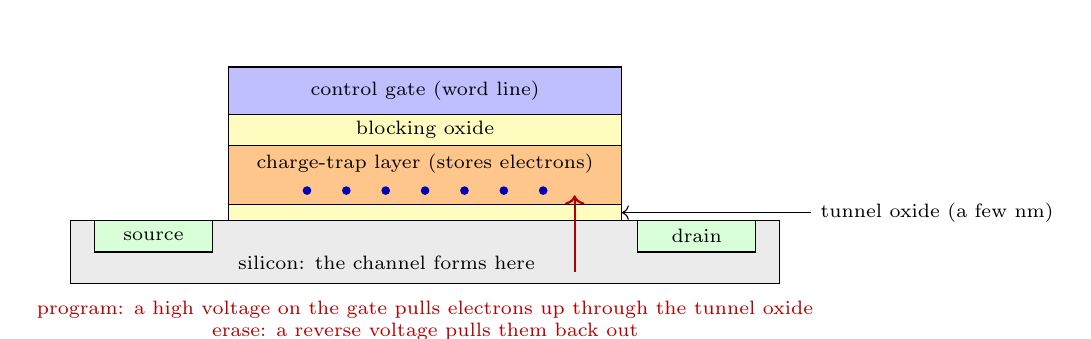
\begin{tikzpicture}[font=\scriptsize]
\draw[fill=black!8] (0,0) rectangle (9.0,0.8);
\node[anchor=south west] at (2.0,0.06) {silicon: the channel forms here};
\draw[fill=green!15] (0.3,0.4) rectangle (1.8,0.8) node[pos=0.5] {source};
\draw[fill=green!15] (7.2,0.4) rectangle (8.7,0.8) node[pos=0.5] {drain};
\draw[fill=yellow!25] (2.0,0.8) rectangle (7.0,1.0);
\draw[fill=orange!45] (2.0,1.0) rectangle (7.0,1.75);
\node at (4.5,1.52) {charge-trap layer (stores electrons)};
\foreach \x in {3.0,3.5,4.0,4.5,5.0,5.5,6.0} \fill[blue!70!black] (\x,1.18) circle (0.055);
\draw[fill=yellow!25] (2.0,1.75) rectangle (7.0,2.15) node[pos=0.5] {blocking oxide};
\draw[fill=blue!25] (2.0,2.15) rectangle (7.0,2.75) node[pos=0.5] {control gate (word line)};
\draw[<-] (7.0,0.9) -- (9.4,0.9) node[right] {tunnel oxide (a few nm)};
\draw[->,thick,red!70!black] (6.4,0.15) -- (6.4,1.12);
\node[red!70!black,anchor=north,align=center] at (4.5,-0.1) {program: a high voltage on the gate pulls electrons up through the tunnel oxide\\erase: a reverse voltage pulls them back out};
\end{tikzpicture}

\small 낸드 셀 하나의 단면 (3D NAND에서 흔한 charge-trap 셀). 갇힌 전자의 양이 트랜지스터의 문턱전압을 바꾸고, 그 차이로 비트를 읽는다.
\end{minipage}
\end{center}

\begin{itemize}[leftmargin=1.5em]
\item \textbf{쓰기} (program): 게이트에 높은 전압 (약 $20$ V)을 걸어, 전자가 수 nm 두께의 얇은 절연막을 뚫고 (양자 터널링) 가두는 층으로 들어가게 한다.
\item \textbf{지우기} (erase): 반대 방향으로 전압을 걸어 전자를 빼낸다. 이것은 블록 (수 MB) 단위로만 할 수 있다 (\ref{sec:m2}절).
\item \textbf{비휘발성}: 전자는 절연막에 둘러싸여 있어 전원이 없어도 수년 동안 갇혀 있다. refresh가 필요 없다.
\item \textbf{수명}: 전자가 절연막을 지날 때마다 막이 조금씩 상한다. 그래서 셀마다 지우고 쓰는 횟수 (P/E cycle)에 한계가 있다.
대략 SLC는 수만$\sim 10$만 번, TLC는 수천 번, QLC는 $1{,}000$번 안팎이다. SSD의 TBW는 이 한계에서 나온다.
\end{itemize}

예전에는 가두는 층이 도체 (polysilicon)인 \textbf{floating gate} 셀을 썼다.
지금의 3D NAND는 대부분 절연체 (질화막)에 전자를 가두는 \textbf{charge-trap} 셀을 쓴다. 셀을 위로 쌓기에 더 알맞기 때문이다.
셀당 비트 수 (SLC$\sim$QLC), 셀을 직렬로 잇는 NAND 구조와 이름의 뜻, 페이지와 블록은 \ref{sec:m2}절에 정리되어 있다.

\paragraph{한눈에 비교.}
\begin{center}
{\small
\begin{tabular}{@{}l>{\raggedright\arraybackslash}p{58mm}>{\raggedright\arraybackslash}p{58mm}@{}}
\toprule
& D램 (DRAM) & 낸드 (NAND flash) \\
\midrule
셀 & 트랜지스터 $1$개 $+$ 커패시터 $1$개 & 전하를 가두는 층이 있는 트랜지스터 $1$개 \\
비트를 나타내는 것 & 커패시터의 전하 & 갇힌 전자가 바꾼 문턱전압 \\
전원을 끄면 & 사라진다 (휘발성, refresh 필요) & 남는다 (비휘발성) \\
읽기 지연 & 약 $100$ ns (CPU에서 본 값) & 약 $50\sim100$ $\mu$s (SSD에서 본 값) \\
쓰기 & 바이트 단위로 바로 덮어씀 & 페이지 단위, 덮어쓰려면 블록을 먼저 지움 \\
쓰기 횟수의 한계 & 사실상 없음 & 셀마다 수백$\sim$수만 번 \\
같은 용량의 가격 & 비싸다 (보통 낸드의 수십 배) & 싸다 \\
쓰이는 곳 & CPU 메모리 (DDR), VRAM (GDDR, HBM), 휴대폰 메모리 (LPDDR) & SSD, USB 메모리, 휴대폰 저장공간 \\
\bottomrule
\end{tabular}}
\end{center}

\begin{mlbox}[{{딥러닝에서: 무엇이 D램에, 무엇이 낸드에 있는가}}]
\begin{itemize}[leftmargin=1.5em]
\item \textbf{D램}: 학습하는 동안 계속 읽고 쓰는 것. GPU의 VRAM (GDDR, HBM)에는 매개변수, 기울기, optimizer 상태, 중간값이 있고,
CPU의 RAM (DDR5)에는 \texttt{DataLoader}가 만드는 미니배치와 운영체제가 보관한 데이터셋 파일 (page cache)이 있다.
\item \textbf{낸드}: 전원이 꺼져도 남아야 하는 것. SSD에 데이터셋, \texttt{torch.save}로 저장한 체크포인트, 코드와 결과 그림이 있다.
\item 학습 중에 꺼지면 D램의 내용은 모두 사라진다. 그래서 체크포인트를 낸드 (SSD)에 \textbf{주기적으로} 저장해 두어야 이어서 학습할 수 있다.
\end{itemize}
\end{mlbox}

\begin{remarkbox}[메모리 반도체 산업]
D램은 삼성전자, SK하이닉스, 마이크론 세 회사가 세계 생산의 대부분을 차지한다. \ref{sec:ddr}절의 HBM도 D램 제품이며, 같은 세 회사가 만든다.
낸드는 삼성전자, SK하이닉스 (자회사 솔리다임 포함), 키옥시아, 마이크론, 샌디스크, YMTC 등이 만든다.
CPU나 GPU처럼 회사마다 설계가 다른 반도체와 달리, 메모리는 JEDEC 규격에 맞춘 \textbf{같은 모양의 제품}을 대량으로 만든다.
그래서 가격이 수요와 공급에 따라 크게 오르내리며, 이것을 \textbf{메모리 사이클}이라고 부른다.
AI 서버가 HBM과 고용량 SSD를 많이 쓰게 되면서, 두 메모리 모두 AI 하드웨어의 중요한 부품이 되었다.
\end{remarkbox}

\subsection{메모리 계층}\label{sec:hierarchy}

빠른 메모리는 작고 비싸며, 큰 메모리는 느리다. 그래서 컴퓨터는 여러 층의 메모리를 쌓아 쓴다.

\begin{center}
\begin{minipage}{\textwidth}\centering
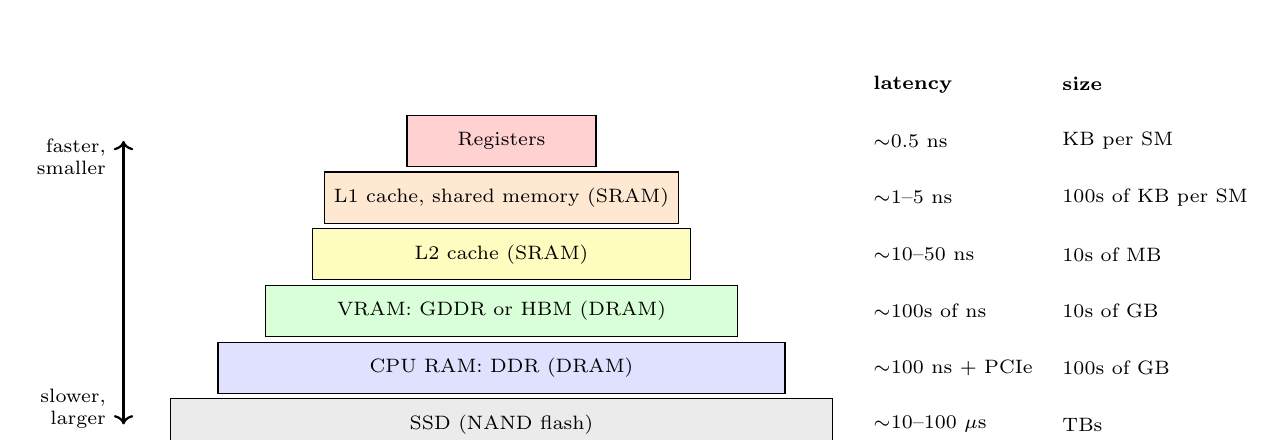
\begin{tikzpicture}[font=\scriptsize]
\foreach \y/\w/\name/\c/\lat/\cap in {
  5/2.4/Registers/red!18/{$\sim$0.5 ns}/{KB per SM},
  4/3.6/{L1 cache, shared memory (SRAM)}/orange!18/{$\sim$1--5 ns}/{100s of KB per SM},
  3/4.8/{L2 cache (SRAM)}/yellow!25/{$\sim$10--50 ns}/{10s of MB},
  2/6.0/{VRAM: GDDR or HBM (DRAM)}/green!15/{$\sim$100s of ns}/{10s of GB},
  1/7.2/{CPU RAM: DDR (DRAM)}/blue!12/{$\sim$100 ns + PCIe}/{100s of GB},
  0/8.4/{SSD (NAND flash)}/black!8/{$\sim$10--100 $\mu$s}/{TBs}} {
  \node[draw,fill=\c,minimum width=\w cm,minimum height=6.5mm] at (0,\y*0.72) {\name};
  \node[anchor=west] at (4.6,\y*0.72) {\lat};
  \node[anchor=west] at (7.0,\y*0.72) {\cap};
}
\node[anchor=west,font=\scriptsize\bfseries] at (4.6,4.32) {latency};
\node[anchor=west,font=\scriptsize\bfseries] at (7.0,4.32) {size};
\draw[<->,thick] (-4.8,0) -- (-4.8,3.6);
\node[anchor=east,align=right] at (-4.9,3.4) {faster,\\smaller};
\node[anchor=east,align=right] at (-4.9,0.2) {slower,\\larger};
\end{tikzpicture}

\small 메모리 계층 (memory hierarchy). 위로 갈수록 빠르고 작다. 숫자는 대략적인 값이다.
\end{minipage}
\end{center}

GPU 프로그램이 빠르려면 자주 쓰는 데이터가 위쪽 층에 머물러야 한다.
cuBLAS나 cuDNN 같은 라이브러리는 행렬을 작은 조각 (tile)으로 잘라 shared memory에 올려 두고 여러 번 재사용하는 방법으로 이것을 한다.
그래서 우리가 직접 짠 반복문보다 라이브러리의 행렬곱이 훨씬 빠르다.

\subsection{대역폭과 지연시간}\label{sec:bandwidth}

메모리와 통로의 성능은 두 가지로 잰다.

\begin{itemize}[leftmargin=1.5em]
\item \textbf{대역폭} (bandwidth): 데이터가 흐르기 시작한 뒤 \textbf{초당 얼마나 많이} 옮기는가. 단위는 GB/s.
\item \textbf{지연시간} (latency): 요청 하나를 보낸 뒤 \textbf{첫 데이터가 오기까지} 얼마나 걸리는가. 단위는 ns.
\end{itemize}

수도관으로 비유하면 대역폭은 관의 \textbf{굵기}, 지연시간은 관의 \textbf{길이}이다.
DRAM의 지연시간은 세대가 바뀌어도 크게 줄지 않았다 (약 $100$ ns). 늘어난 것은 대역폭이다.
그래서 DRAM은 연속된 주소를 덩어리 (burst)로 한꺼번에 읽을 때 가장 빠르다.
PyTorch에서 텐서가 연속 (\texttt{contiguous()})이 아니면 느려지는 이유도 여기에 있다.

\begin{remarkbox}[왜 ``대역폭''인가]
bandwidth는 원래 신호처리와 통신의 말로, 통로가 통과시키는 \textbf{주파수 범위의 폭}이다 (예: $0\sim20$ kHz이면 $20$ kHz).
Nyquist와 Shannon에 따르면 통로가 초당 보낼 수 있는 정보량은 이 폭에 비례한다.
그래서 ``대역이 넓다 = 많이 보낸다''가 되었고, 컴퓨터에서는 \textbf{초당 전송량}의 뜻으로 굳었다.
\end{remarkbox}

\begin{center}
\begin{minipage}{\textwidth}\centering
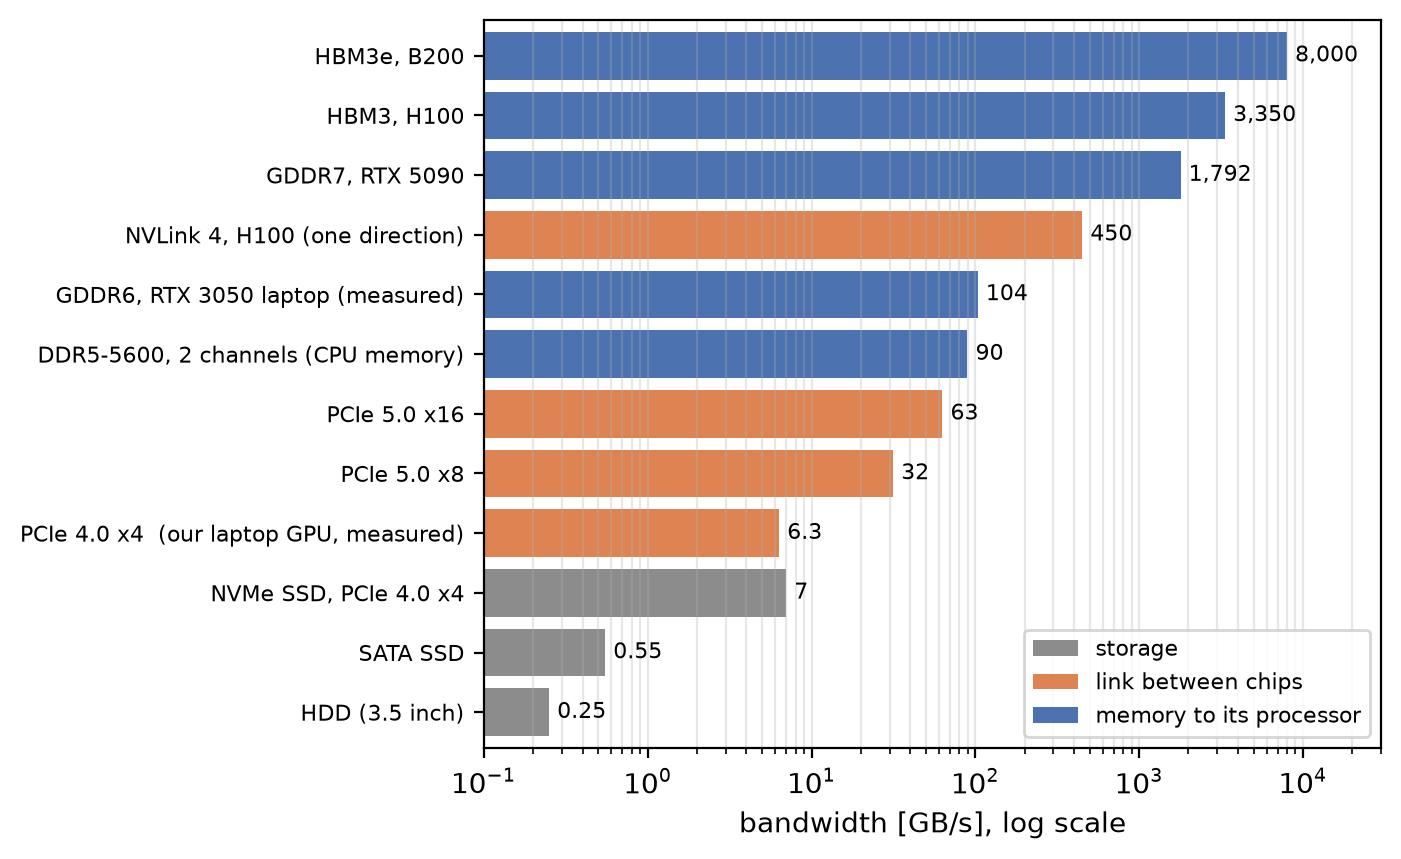
\includegraphics[width=0.86\textwidth]{figures/bandwidth_ladder.png}

\small 데이터가 지나는 여러 통로의 대역폭 (로그 눈금, 한 방향). 회색은 저장장치, 주황은 칩 사이의 연결, 파랑은 메모리와 그 프로세서 사이이다.
``measured''는 \texttt{gpu\_bench.py}로 강의자의 노트북에서 잰 값이고, 나머지는 제조사가 발표한 사양 값이다 (\texttt{hardware\_charts.py}).
\end{minipage}
\end{center}

\subsection{DDR, GDDR, HBM: 이름의 뜻}\label{sec:ddr}

메모리의 이름은 약어를 차례로 붙여 만든 것이라 뒤에서부터 풀면 뜻이 나온다.

\begin{itemize}[leftmargin=1.5em]
\item \textbf{SDRAM} (Synchronous DRAM): 메모리를 시스템의 \textbf{클럭에 맞추어} 동작시킨 DRAM (1990년대).
\item \textbf{DDR} (Double Data Rate): 클럭 신호가 \textbf{올라갈 때와 내려갈 때 모두} 데이터를 보내 같은 클럭으로 전송량을 $2$배로 한 SDRAM (2000년경).
그 뒤 세대마다 번호를 붙여 DDR2, DDR3, DDR4, \textbf{DDR5} (2020년 표준)가 되었다. PC의 메인 메모리이다.
\item \textbf{GDDR} (Graphics DDR): 그래픽카드용으로 변형한 DDR. 핀 하나당 속도를 매우 높였다.
\textbf{세대 번호는 DDR과 따로} 간다. GDDR7이 DDR5보다 두 세대 앞선 것이 아니다.
GDDR6X는 신호를 $4$단계 (PAM4)로, GDDR7은 $3$단계 (PAM3)로 보내 한 번에 $1$비트보다 많이 싣는다.
\item \textbf{HBM} (High Bandwidth Memory): DRAM 칩을 여러 층 \textbf{쌓아} (stack) GPU 바로 옆에 붙인 메모리.
AMD와 SK하이닉스가 개발하여 2013년에 표준이 되었고, 2015년 AMD Radeon R9 Fury에 처음 쓰였다.
세대는 HBM, HBM2, HBM2E, HBM3, \textbf{HBM3E}, HBM4이다. 끝의 \textbf{E}는 Extended로, 새 세대가 아니라 같은 세대 안의 개량판이다.
\item \textbf{LPDDR} (Low Power DDR): 스마트폰과 노트북용 저전력 DDR.
\item \textbf{JEDEC} (Joint Electron Device Engineering Council): 이 규격들을 정하는 반도체 업계의 표준 단체이다. 그래서 같은 규격이면 제조사가 달라도 호환된다.
\end{itemize}

\paragraph{메모리 이름의 숫자 읽기.}
\textbf{DDR5-5600}은 초당 $5600$ MT (mega-transfers, 백만 번 전송)이다. 흔히 ``5600 MHz''라고 부르지만 정확히는 전송 횟수이다.
모듈 하나의 폭은 $64$비트 $=8$바이트이므로 모듈 하나의 대역폭은 $5600\times8=44{,}800$ MB/s이고, 이것을 \textbf{PC5-44800}이라고 쓴다.
데스크톱 CPU는 메모리 채널이 $2$개여서 약 $90$ GB/s이다.
(채널과 DIMM은 2.2절 참고.)

\begin{center}
{\small
\begin{tabular}{@{}lllll@{}}
\toprule
종류 & 쓰이는 곳 & 연결 폭 & 대역폭의 예 & 특징 \\
\midrule
DDR5 & CPU 메모리 & $64$비트 $\times$ 채널 & $\sim$90 GB/s ($2$채널) & 크고 쌈, 교체 가능 \\
GDDR7 & 그래픽카드 & $32$비트 $\times$ 칩 & $1{,}792$ GB/s (RTX 5090) & 좁고 빠름 \\
HBM3e & 데이터센터 GPU & $1024$비트 $\times$ stack & $\sim$8,000 GB/s (B200) & 넓고 비쌈 \\
LPDDR5X & 휴대폰, 노트북 & 칩 단위 & 수십$\sim$수백 GB/s & 저전력 \\
\bottomrule
\end{tabular}}
\end{center}

\paragraph{GDDR과 HBM의 배치.}
GDDR은 칩을 GPU 주변의 기판에 펼쳐 놓고, 칩마다 $32$비트의 좁고 아주 빠른 통로로 잇는다.
HBM은 DRAM을 위로 쌓아 GPU와 \textbf{같은 패키지 안}에 수 mm 거리로 붙인다. 거리가 짧아 배선을 촘촘히 깔 수 있으므로 stack 하나가 $1024$비트 폭이다.
도로로 비유하면 GDDR은 몇 차선의 초고속도로, HBM은 수천 차선의 도로이다.

\begin{center}
\begin{minipage}{\textwidth}\centering
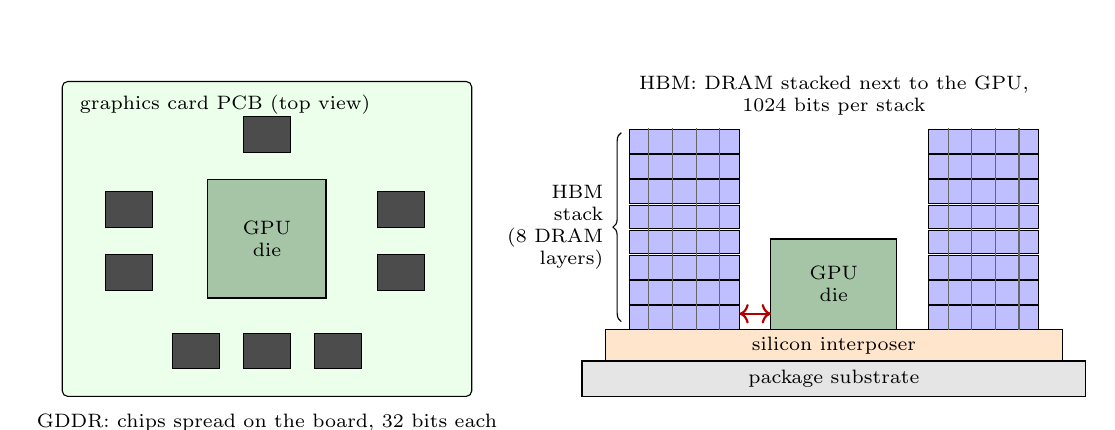
\begin{tikzpicture}[font=\scriptsize]
% ---- GDDR: top view ----
\begin{scope}
\draw[fill=green!8,rounded corners=2pt] (0,0) rectangle (5.2,4.0);
\node[anchor=north west] at (0.1,3.95) {graphics card PCB (top view)};
\draw[fill=green!35!black!35,draw=black] (1.85,1.25) rectangle (3.35,2.75);
\node[align=center] at (2.6,2.0) {GPU\\die};
\foreach \x/\y in {0.55/1.35,0.55/2.15,4.0/1.35,4.0/2.15,1.4/0.35,2.3/0.35,3.2/0.35,2.3/3.1} {
  \draw[fill=black!70] (\x,\y) rectangle ++(0.6,0.45);
}
\node[anchor=north] at (2.6,-0.1) {GDDR: chips spread on the board, 32 bits each};
\end{scope}
% ---- HBM: cross section ----
\begin{scope}[xshift=6.6cm]
\draw[fill=black!10] (0,0) rectangle (6.4,0.45) node[pos=0.5] {package substrate};
\draw[fill=orange!20] (0.3,0.45) rectangle (6.1,0.85) node[pos=0.5] {silicon interposer};
\draw[fill=green!35!black!35] (2.4,0.85) rectangle (4.0,2.0) node[pos=0.5,align=center] {GPU\\die};
\foreach \x in {0.6,4.4} {
  \foreach \k in {0,...,7} \draw[fill=blue!25] (\x,0.85+\k*0.32) rectangle ++(1.4,0.3);
  \foreach \t in {0.25,0.55,0.85,1.15} \draw[black!60] (\x+\t,0.85) -- (\x+\t,0.85+8*0.32);
}
\draw[decorate,decoration={brace,amplitude=3pt}] (0.5,0.95) -- (0.5,3.35) node[midway,left=3pt,align=right] {HBM\\stack\\(8 DRAM\\layers)};
\draw[<->,thick,red!70!black] (2.0,1.05) -- (2.4,1.05);
\node[anchor=south,align=center] at (3.2,3.45) {HBM: DRAM stacked next to the GPU,\\1024 bits per stack};
\end{scope}
\end{tikzpicture}

\small 왼쪽: GDDR (위에서 본 모습). 오른쪽: HBM (단면). HBM의 층 사이는 실리콘을 관통하는 수직 배선 (TSV, through-silicon via)으로 잇는다.
\end{minipage}
\end{center}

\begin{center}
\photo{gpu_pcb_die_gddr.jpg}{0.47\textwidth}{냉각기를 뗀 그래픽카드 (GTX 780). 가운데 GPU 칩 주위에 GDDR5 칩들이 있다.}\hfill
\photo{gddr6_chips_closeup.png}{0.47\textwidth}{GPU 패키지 옆의 GDDR6 칩 (RTX 3060)}\\[0.8em]
\photo{hbm_fiji_package.jpg}{0.47\textwidth}{HBM을 쓴 GPU 패키지 (AMD Fiji, 2015). 가운데 GPU 양옆에 HBM stack $4$개가 interposer 위에 붙어 있다.}\hfill
\photo{hbm_stack_crosssection.jpg}{0.47\textwidth}{HBM stack을 자른 단면의 현미경 사진 (Tesla P100). DRAM 층이 위로 쌓여 있다.}
\end{center}

HBM은 SK하이닉스, 삼성전자, 마이크론 세 회사만 만든다. AI용 GPU의 수요 때문에 HBM은 반도체 산업에서 가장 중요한 제품 중 하나가 되었다.

\subsection{비트 수: 폭과 속도}\label{sec:width}

``채널당 $64$비트'', ``stack당 $1024$비트''의 비트 수는 \textbf{동시에 보내는 비트의 수}, 즉 나란히 깔린 \textbf{데이터 전선의 가닥 수}이다.
DDR5 채널에는 데이터선이 $64$가닥 있고, 전선 하나가 한 번 (한 박자)에 $1$비트를 나른다.
그래서 전송 한 번에 $64$비트 $=8$바이트가 움직인다. 이 비트 수를 통로의 \textbf{폭} (width)이라고 한다.

전선의 양 끝은 칩이나 커넥터의 금속 접점 하나에 닿는다. 이 접점 하나를 \textbf{핀} (pin)이라고 한다 (2.4절의 CPU 아랫면 사진에 보이는 것들이다).
전선 하나에 핀 하나이므로, 데이터선 $64$가닥은 \textbf{핀 $64$개}이다. 그래서 전선 하나의 속도를 흔히 \textbf{핀당 속도}라고 부른다.
DDR5 DIMM의 접점 $288$개 중 데이터선은 일부이고, 나머지는 주소, 명령, 클럭, 전원, 접지이다.
PCIe는 잡음에 강하도록 신호 하나를 전선 \textbf{두 가닥} (차동 신호, differential pair)으로 보내므로, lane 하나는 방향마다 핀 $2$개, 양방향 핀 $4$개를 쓴다.

\begin{center}
\begin{minipage}{\textwidth}\centering
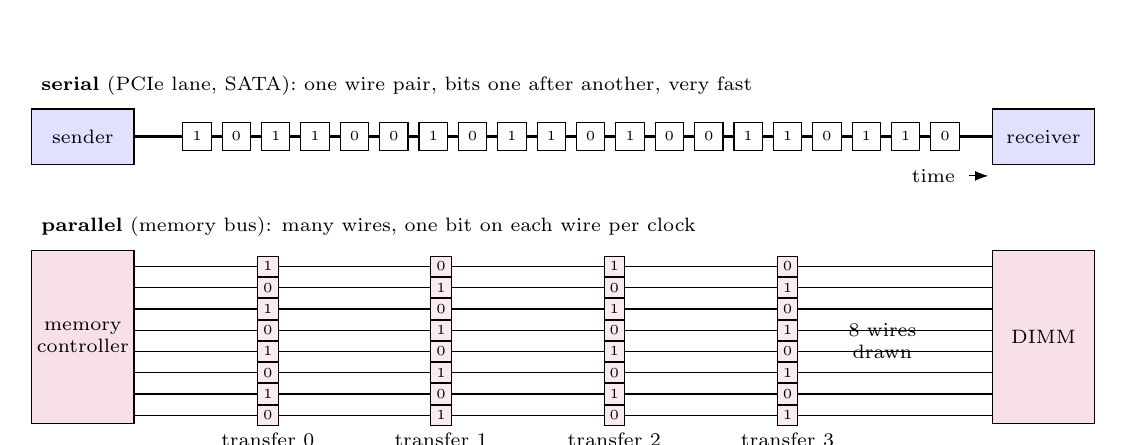
\begin{tikzpicture}[font=\scriptsize,>=Latex]
\tikzset{bit/.style={draw,minimum size=3.6mm,inner sep=0pt,font=\tiny}}
% serial
\node[anchor=west] at (0,3.55) {\textbf{serial} (PCIe lane, SATA): one wire pair, bits one after another, very fast};
\draw[fill=blue!12] (0,2.55) rectangle (1.3,3.25) node[pos=0.5] {sender};
\draw[fill=blue!12] (12.2,2.55) rectangle (13.5,3.25) node[pos=0.5] {receiver};
\draw[thick] (1.3,2.9) -- (12.2,2.9);
\foreach \b [count=\i] in {1,0,1,1,0,0,1,0,1,1,0,1,0,0,1,1,0,1,1,0} {
  \node[bit,fill=white] at (1.6+\i*0.5,2.9) {\b};
}
\draw[->] (11.9,2.4) -- (12.15,2.4);
\node[anchor=east] at (11.85,2.4) {time};
% parallel
\node[anchor=west] at (0,1.75) {\textbf{parallel} (memory bus): many wires, one bit on each wire per clock};
\draw[fill=purple!12] (0,-0.75) rectangle (1.3,1.45) node[pos=0.5,align=center] {memory\\controller};
\draw[fill=purple!12] (12.2,-0.75) rectangle (13.5,1.45) node[pos=0.5] {DIMM};
\foreach \k [count=\j] in {0,...,7} {
  \pgfmathsetmacro{\y}{1.25-\k*0.27}
  \draw (1.3,\y) -- (12.2,\y);
}
\foreach \col/\x in {0/3.0,1/5.2,2/7.4,3/9.6} {
  \foreach \k in {0,...,7} {
    \pgfmathsetmacro{\y}{1.25-\k*0.27}
    \pgfmathtruncatemacro{\v}{mod(\k*3+\col*5+1,2)}
    \node[bit,fill=purple!8,minimum size=2.6mm] at (\x,\y) {\v};
  }
  \node at (\x,-0.95) {transfer \col};
}
\node[align=center,anchor=west] at (10.25,0.3) {8 wires\\drawn};
\end{tikzpicture}

\small 직렬 전송과 병렬 전송. 병렬 전송에서 한 열이 한 번의 전송이다. 실제 DDR5 채널은 $64$가닥, HBM stack은 $1024$가닥이다.
\end{minipage}
\end{center}

대역폭은 \textbf{폭과 속도의 곱}이다.
\[
\text{대역폭 [GB/s]} = \frac{\text{폭 [비트]} \times \text{전선 하나의 속도 [Gbit/s]}}{8} .
\]
\begin{center}
{\small
\begin{tabular}{@{}lrrr@{}}
\toprule
통로 & 폭 & 전선 하나의 속도 & 대역폭 \\
\midrule
PCIe 5.0, lane 하나 (한 방향) & $1$비트 & $32$ Gbit/s & $\approx4$ GB/s \\
DDR5-5600, 채널 하나 & $64$비트 & $5.6$ Gbit/s & $44.8$ GB/s \\
GDDR7, RTX 5090 ($32$비트 칩 $16$개) & $512$비트 & $28$ Gbit/s & $1{,}792$ GB/s \\
HBM3e, stack 하나 & $1024$비트 & $\sim8$ Gbit/s & $\sim1$ TB/s \\
HBM3e, B200 (stack $8$개) & $8192$비트 & $\sim8$ Gbit/s & $\sim8$ TB/s \\
\bottomrule
\end{tabular}}
\end{center}

\begin{center}
\begin{minipage}{\textwidth}\centering
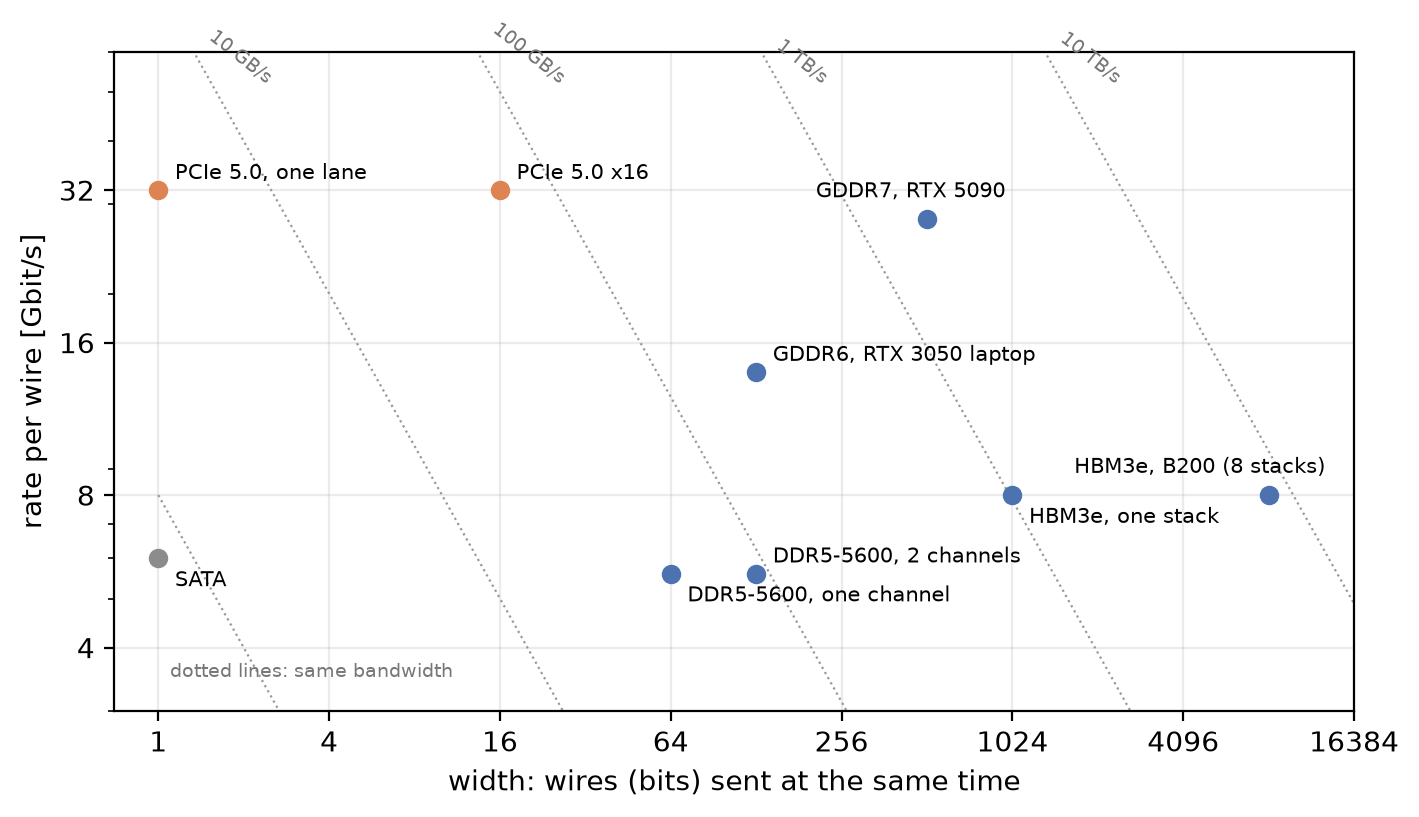
\includegraphics[width=0.84\textwidth]{figures/bus_width_rate.png}

\small 여러 통로의 폭 (가로)과 전선 하나의 속도 (세로), 둘 다 로그 눈금. 점선 위의 통로들은 대역폭이 같다.
GDDR과 PCIe는 위쪽 (좁고 빠름), HBM은 오른쪽 (넓고 느림)에 있다 (\texttt{hardware\_charts.py}).
\end{minipage}
\end{center}

대역폭을 키우는 방법은 두 가지이다.
\begin{itemize}[leftmargin=1.5em]
\item \textbf{좁고 빠르게} (GDDR, PCIe): 전선 하나의 속도를 극단적으로 높인다. 신호를 $2$단계보다 많게 (PAM3, PAM4) 하여 한 박자에 더 많이 싣기도 한다.
\item \textbf{넓고 느리게} (HBM): 전선 수를 극단적으로 늘린다. 전선 하나의 속도는 GDDR7의 $1/3$ 정도지만 폭이 수십 배이다.
속도가 느리고 거리가 짧아서, 같은 양의 데이터를 보내는 데 드는 \textbf{전력도 적다}.
\end{itemize}

\paragraph{왜 모든 통로를 넓게 만들지 않는가?}
병렬 전선은 길어질수록 가닥마다 신호가 도착하는 시간이 조금씩 어긋나고 (skew), 옆 선끼리 간섭한다.
그래서 길게 이어야 하는 통로 (그래픽카드 슬롯, 저장장치 케이블)는 \textbf{직렬}로 바뀌었다. 옛 PCI와 PATA가 각각 PCIe와 SATA가 된 것이 그 예이다 (2.3절).
메모리는 CPU 바로 옆이라 병렬을 유지하고, HBM은 GPU에서 수 mm 떨어진 실리콘 위라서 수천 가닥까지 넓힐 수 있다.
일반 기판 위에서는 전선을 그렇게 촘촘히 깔 수 없다.

\begin{remarkbox}[``64비트 CPU''와는 다른 이야기]
``64비트 CPU'', ``64비트 운영체제''의 64비트는 CPU가 한 번에 다루는 정수와 메모리 주소의 크기 (레지스터의 폭)이다.
메모리 채널의 $64$비트는 데이터 전선의 가닥 수이다. 숫자가 같지만 서로 관계가 없다.
또 \texttt{float32}의 $32$비트는 숫자 하나를 저장하는 비트 수이다 (5절). 같은 ``비트''라도 무엇의 개수인지 확인해야 한다.
\end{remarkbox}

\begin{remarkbox}[덧붙임: DDR5의 64비트]
DDR5는 채널의 $64$비트를 $32$비트 두 개 (subchannel)로 나누어, 각자 따로 주소를 받아 일하게 한다.
한 번 요청하면 $32$비트씩 $16$번을 연달아 보내 $64$바이트가 온다. 이 크기는 CPU 캐시가 한 번에 다루는 단위 (cache line)와 같다.
\end{remarkbox}

% =================================================
\section{GPU의 안}\label{sec:inside}
% =================================================

\subsection{CPU와 GPU}\label{sec:cpu_gpu}

CPU와 GPU의 칩은 지름 $300$ mm의 실리콘 \textbf{웨이퍼} (wafer) 위에 같은 회로 수백 개를 한꺼번에 만든 뒤 잘라 낸 조각이다. 이 조각을 \textbf{die}라고 한다.
die가 클수록 웨이퍼 한 장에서 나오는 칩이 적고, 불량이 섞일 확률이 커서 비싸다.
RTX 5090의 die (GB202)는 약 $750$ mm$^2$로, 손톱 몇 개를 합친 크기이다.

\begin{center}
\photo{wafer_300mm_dies.jpg}{0.36\textwidth}{$300$ mm 웨이퍼. 격자 하나하나가 칩 (die)이다.}
\end{center}

\begin{center}
\begin{minipage}{\textwidth}\centering
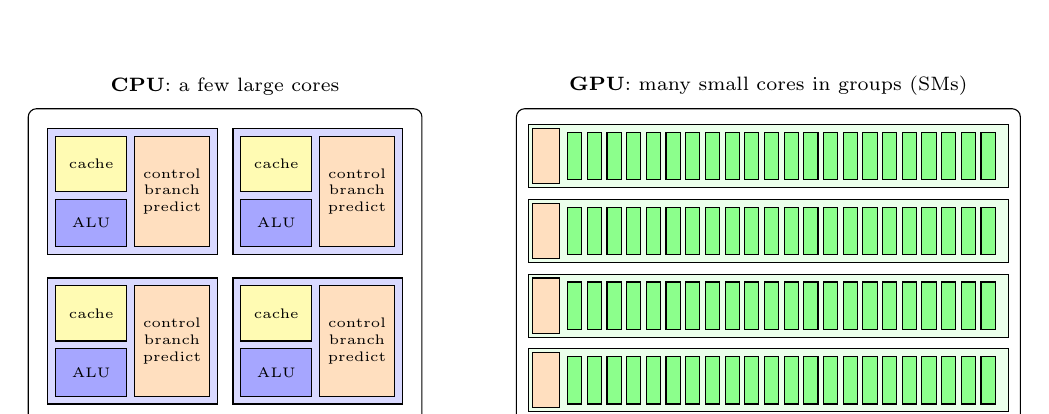
\begin{tikzpicture}[font=\scriptsize]
\begin{scope}
\draw[rounded corners=3pt] (0,0) rectangle (5.0,4.0);
\node[anchor=south] at (2.5,4.05) {\textbf{CPU}: a few large cores};
\foreach \x/\y in {0.25/2.15,2.6/2.15,0.25/0.25,2.6/0.25} {
  \draw[fill=blue!15] (\x,\y) rectangle ++(2.15,1.6);
  \draw[fill=blue!35] (\x+0.1,\y+0.1) rectangle ++(0.9,0.6) node[pos=0.5,font=\tiny] {ALU};
  \draw[fill=orange!25] (\x+1.1,\y+0.1) rectangle ++(0.95,1.4) node[pos=0.5,font=\tiny,align=center] {control\\branch\\predict};
  \draw[fill=yellow!30] (\x+0.1,\y+0.8) rectangle ++(0.9,0.7) node[pos=0.5,font=\tiny] {cache};
}
\end{scope}
\begin{scope}[xshift=6.2cm]
\draw[rounded corners=3pt] (0,0) rectangle (6.4,4.0);
\node[anchor=south] at (3.2,4.05) {\textbf{GPU}: many small cores in groups (SMs)};
\foreach \j in {0,...,3} {
  \draw[fill=green!8] (0.15,0.15+\j*0.95) rectangle (6.25,0.95+\j*0.95);
  \draw[fill=orange!25] (0.2,0.2+\j*0.95) rectangle ++(0.35,0.7);
  \foreach \i in {0,...,21} \draw[fill=green!45] (0.65+\i*0.25,0.25+\j*0.95) rectangle ++(0.18,0.6);
}
\end{scope}
\end{tikzpicture}

\small CPU는 복잡한 명령을 빠르게 처리하는 큰 코어 몇 개 (그리고 큰 캐시와 제어 회로), GPU는 단순한 곱셈-덧셈을 하는 작은 코어 수천 개를 가진다.
GPU의 한 줄이 SM 하나이고, 주황색이 그 SM의 명령 장치 (scheduler)이다.
\end{minipage}
\end{center}

CPU는 분기 (if문)가 많고 순서대로 해야 하는 일을 빨리 처리하도록 설계되었다. 코어 하나가 명령을 미리 예측하고 순서를 바꾸어 실행하는 복잡한 회로를 가진다.
GPU는 \textbf{같은 계산을 아주 많은 데이터에 동시에} 하도록 설계되었다. 행렬곱 $C=AB$의 원소 $c_{ij}=\sum_k a_{ik}b_{kj}$는 서로 독립이므로 GPU에 꼭 맞는다 (딥러닝 노트 3.2절).

\subsection{SM, CUDA core, warp}\label{sec:sm}

GPU 칩은 \textbf{SM} (Streaming Multiprocessor)이라는 같은 블록 수십$\sim$수백 개로 이루어진다. CPU의 코어에 해당하는 것은 SM이다.

\begin{center}
\begin{minipage}{\textwidth}\centering
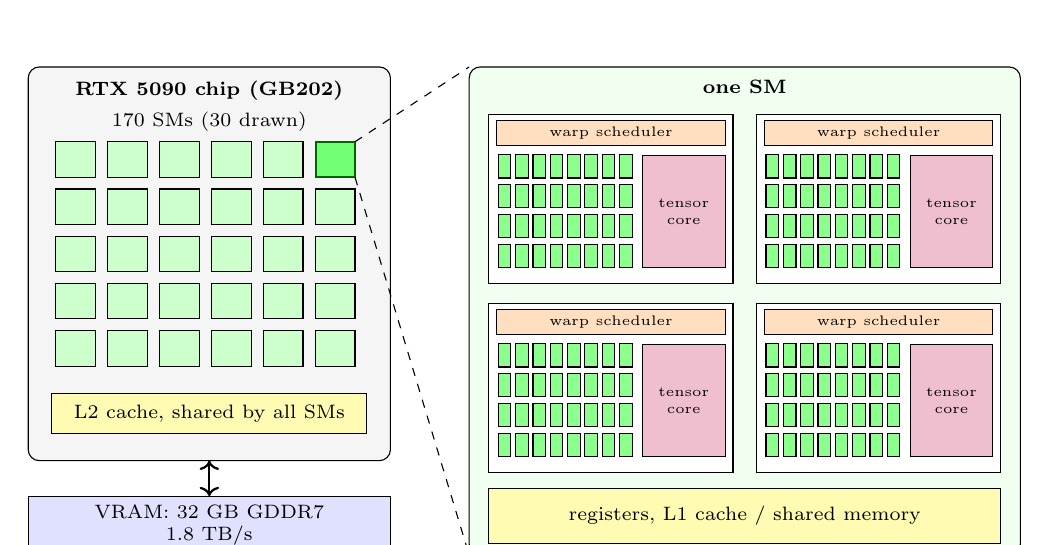
\begin{tikzpicture}[font=\scriptsize]
% chip
\draw[fill=black!4,rounded corners=4pt] (0,0) rectangle (4.6,5.0);
\node[anchor=north] at (2.3,4.95) {\textbf{RTX 5090 chip (GB202)}};
\foreach \i in {0,...,5} \foreach \j in {0,...,4} {
  \draw[fill=green!20] (0.35+\i*0.66,1.2+\j*0.6) rectangle ++(0.5,0.45);
}
\draw[fill=green!55,draw=green!40!black,thick] (0.35+5*0.66,1.2+4*0.6) rectangle ++(0.5,0.45);
\node at (2.3,4.3) {170 SMs (30 drawn)};
\draw[fill=yellow!30] (0.3,0.35) rectangle (4.3,0.85) node[pos=0.5] {L2 cache, shared by all SMs};
\draw[fill=blue!12] (0,-1.2) rectangle (4.6,-0.45) node[pos=0.5,align=center] {VRAM: 32 GB GDDR7\\1.8 TB/s};
\draw[<->,thick] (2.3,0) -- (2.3,-0.45);
% zoom
\draw[dashed] (0.35+5*0.66+0.5,1.2+4*0.6+0.45) -- (5.6,5.0);
\draw[dashed] (0.35+5*0.66+0.5,1.2+4*0.6) -- (5.6,-1.2);
\draw[fill=green!6,rounded corners=4pt] (5.6,-1.2) rectangle (12.6,5.0);
\node[anchor=north] at (9.1,4.95) {\textbf{one SM}};
\foreach \px/\py in {5.85/2.25,9.25/2.25,5.85/-0.15,9.25/-0.15} {
  \draw[fill=white] (\px,\py) rectangle ++(3.1,2.15);
  \draw[fill=orange!25] (\px+0.1,\py+1.75) rectangle ++(2.9,0.32) node[pos=0.5,font=\tiny] {warp scheduler};
  \foreach \r in {0,...,3} \foreach \c in {0,...,7}
    \draw[fill=green!45] (\px+0.12+\c*0.22,\py+0.2+\r*0.38) rectangle ++(0.16,0.3);
  \draw[fill=purple!25] (\px+1.95,\py+0.2) rectangle ++(1.05,1.42) node[pos=0.5,font=\tiny,align=center] {tensor\\core};
}
\draw[fill=yellow!30] (5.85,-1.05) rectangle (12.35,-0.35) node[pos=0.5] {registers, L1 cache / shared memory};
\end{tikzpicture}

\small RTX 5090의 구조. 칩에 SM $170$개가 있고, SM 하나는 네 부분으로 나뉘며 각 부분에 CUDA core $32$개와 tensor core $1$개가 있다.
\end{minipage}
\end{center}

\begin{itemize}[leftmargin=1.5em]
\item \textbf{CUDA core}: SM 안의 \textbf{FP32 계산기 한 칸}을 부르는 NVIDIA의 이름이다. 매 클럭에 $d=a\times b+c$ 하나 (FMA, fused multiply-add)를 계산한다.
CPU의 ``코어''와 달리 혼자서 명령을 읽지 못한다.
\item \textbf{warp}: \textbf{$32$개의 thread} 묶음이다. 한 warp의 thread들은 \textbf{같은 명령을 동시에}, 서로 다른 데이터에 실행한다.
이 방식을 \textbf{SIMT} (Single Instruction, Multiple Threads)라고 한다. warp scheduler가 매 클럭 준비된 warp를 골라 실행한다.
\item 한 warp 안에서 if문의 갈래가 나뉘면 (warp divergence) 두 갈래를 차례로 실행해야 해서 느려진다. GPU가 분기가 많은 일에 약한 이유이다.
\end{itemize}

\paragraph{사양표의 TFLOPS 계산하기.}
RTX 5090은 SM $170$개 $\times$ CUDA core $128$개 $=21{,}760$개의 CUDA core를 가지고, 최대 클럭은 약 $2.41$ GHz이다.
FMA 하나를 곱셈과 덧셈 $2$번의 연산으로 세면
\[
21{,}760 \times 2 \times 2.41\times10^{9} \approx 1.05\times10^{14}\ \text{FLOPS} = 105\ \text{TFLOPS (FP32)} .
\]
사양표의 FP32 성능은 이렇게 계산한 \textbf{이론상 최대값}이다 (6절).

\subsection{Tensor core}\label{sec:tensorcore}

\textbf{tensor core}는 \textbf{작은 행렬의 곱}을 통째로 계산하는 전용 회로이다. 딥러닝의 계산 대부분이 행렬곱이므로, 그 일만 매우 빠르게 하도록 따로 만들었다.
2017년 V100 (Volta)에 처음 들어갔다. 이름은 ``tensor''이지만 하는 일은 행렬곱이다.

\begin{center}
\begin{minipage}{\textwidth}\centering
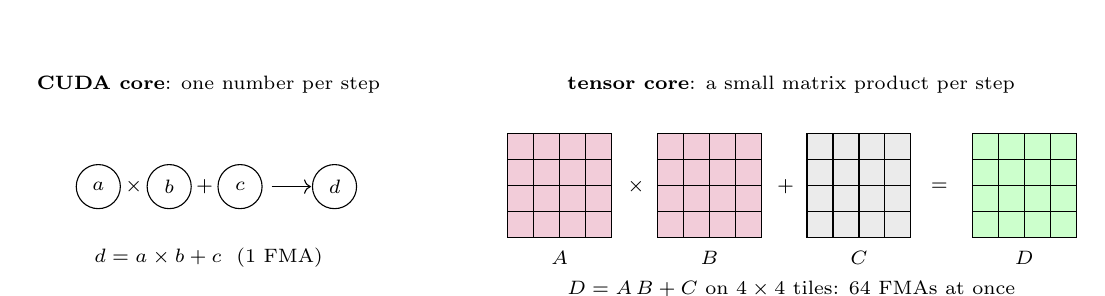
\begin{tikzpicture}[font=\scriptsize]
\begin{scope}
\node at (1.4,2.5) {\textbf{CUDA core}: one number per step};
\foreach \x/\t in {0/a,0.9/b,1.8/c} \draw (\x,1.2) circle (0.28) node {$\t$};
\node at (0.45,1.2) {$\times$}; \node at (1.35,1.2) {$+$};
\draw[->] (2.2,1.2) -- (2.7,1.2); \draw (3.0,1.2) circle (0.28) node {$d$};
\node at (1.4,0.3) {$d = a\times b + c$ \ (1 FMA)};
\end{scope}
\begin{scope}[xshift=5.2cm]
\node at (3.6,2.5) {\textbf{tensor core}: a small matrix product per step};
\foreach \ox/\name/\col in {0/A/purple!20,1.9/B/purple!20,3.8/C/black!8,5.9/D/green!20} {
  \foreach \i in {0,...,3} \foreach \j in {0,...,3} \draw[fill=\col] (\ox+\i*0.33,0.55+\j*0.33) rectangle ++(0.33,0.33);
  \node at (\ox+0.66,0.3) {$\name$};
}
\node at (1.63,1.2) {$\times$}; \node at (3.53,1.2) {$+$}; \node at (5.48,1.2) {$=$};
\node at (3.6,-0.1) {$D = A\,B + C$ on $4\times4$ tiles: 64 FMAs at once};
\end{scope}
\end{tikzpicture}

\small CUDA core와 tensor core. 실제 tensor core가 한 번에 처리하는 조각의 크기는 세대마다 다르고 더 크다.
\end{minipage}
\end{center}

tensor core는 보통 \textbf{입력은 낮은 정밀도} (TF32, BF16, FP16, FP8, FP4)로 받고, \textbf{더하기 (누적)는 높은 정밀도} (FP32)로 한다.
곱셈은 거칠게 해도 결과에 큰 영향이 없고, 오차는 덧셈을 쌓을 때 커지기 쉽다는 점을 이용한 설계이다.
그래서 \textbf{순수 FP32 행렬곱은 tensor core를 쓰지 못한다}. 숫자 형식을 바꾸어야 쓸 수 있다 (5절).
tensor core는 행렬곱과 합성곱만 담당하고, 활성화 함수나 정규화 같은 원소별 계산은 CUDA core가 한다.

\subsection{VRAM에는 무엇이 들어가는가}\label{sec:vram}

학습이 가능한지는 VRAM \textbf{용량}이 먼저 정한다. 매개변수가 $P$개인 모델을 Adam으로 \texttt{float32} 학습하면 VRAM에 다음이 올라간다.

\begin{center}
{\small
\begin{tabular}{@{}lr@{}}
\toprule
항목 & 매개변수 하나당 \\
\midrule
매개변수 $W$ & $4$ 바이트 \\
기울기 $\partial L/\partial W$ & $4$ 바이트 \\
Adam의 $m$, $v$ (학습 관련 기술 노트) & $8$ 바이트 \\
\midrule
합계 & $16$ 바이트 \\
\bottomrule
\end{tabular}}
\end{center}

여기에 역전파를 위해 저장하는 \textbf{중간값} (activation)이 더해진다. 중간값은 미니배치 크기와 입력 크기에 비례하고, 합성곱 신경망에서는 매개변수보다 커지는 일이 흔하다.
예를 들어 $P=10$억 ($10^9$)이면 매개변수와 Adam 상태만으로 $16$ GB이다. VRAM $32$ GB인 RTX 5090에 중간값까지 넣으면 빠듯하다.
VRAM이 모자라면 \texttt{CUDA out of memory} 오류가 나고, 미니배치를 줄이거나 16비트 형식 (5절)을 쓰거나 GPU 여러 장에 나누어야 한다.

\begin{remarkbox}[GPU 두 장이면 VRAM이 두 배?]
아니다. 32 GB GPU 두 장이 64 GB GPU 하나처럼 동작하지는 않는다.
데이터 병렬 (딥러닝 노트 3.3절)에서는 GPU마다 \textbf{모델 전체를 복사}해 두므로 모델의 크기 한계는 그대로이다.
모델 자체를 나누어 올리려면 모델 병렬이나 FSDP (Fully Sharded Data Parallel) 같은 방법을 따로 써야 한다.
\end{remarkbox}

% =================================================
\section{숫자 형식과 정밀도}\label{sec:formats}
% =================================================

\subsection{부동소수점수의 구조}\label{sec:float}

컴퓨터는 실수를 과학적 표기법처럼 저장한다.
\[
x = (-1)^{s}\times 1.m_1m_2\cdots m_p \,(\text{2진수}) \times 2^{\,e-\text{bias}} .
\]
\textbf{부호} (sign) $s$ $1$비트, \textbf{지수} (exponent) $e$, \textbf{가수} (mantissa) $m$으로 나뉜다.
지수의 비트 수가 \textbf{표현할 수 있는 범위}를, 가수의 비트 수가 \textbf{정밀도} (유효숫자)를 정한다.
이름의 FP는 floating point, 뒤의 숫자는 전체 비트 수이다.

\begin{center}
\begin{minipage}{\textwidth}\centering
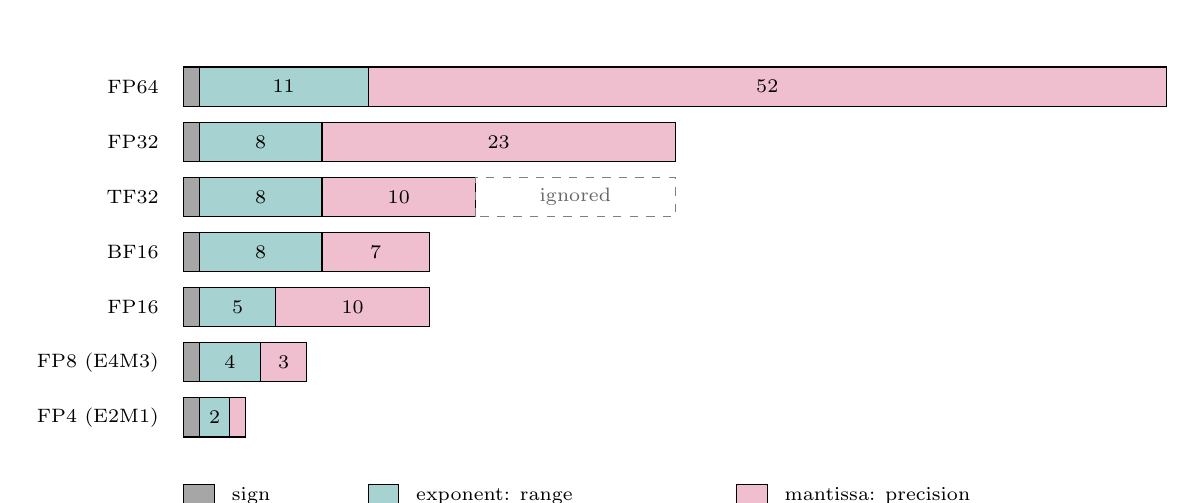
\begin{tikzpicture}[font=\scriptsize,x=1.95mm,y=1mm]
\foreach \row/\name/\e/\m/\pad in {
  0/FP64/11/52/0, 1/FP32/8/23/0, 2/TF32/8/10/13, 3/BF16/8/7/0, 4/FP16/5/10/0, 5/{FP8 (E4M3)}/4/3/0, 6/{FP4 (E2M1)}/2/1/0} {
  \pgfmathsetmacro{\y}{-\row*7}
  \node[anchor=east] at (-1,\y+2.5) {\name};
  \draw[fill=black!35] (0,\y) rectangle (1,\y+5);
  \draw[fill=teal!35] (1,\y) rectangle (1+\e,\y+5);
  \node at (1+\e/2,\y+2.5) {\e};
  \draw[fill=purple!25] (1+\e,\y) rectangle (1+\e+\m,\y+5);
  \ifnum\m>2 \node at (1+\e+\m/2,\y+2.5) {\m}; \fi
  \ifnum\pad>0
    \draw[dashed,black!50] (1+\e+\m,\y) rectangle (1+\e+\m+\pad,\y+5);
    \node[black!60] at (1+\e+\m+\pad/2,\y+2.5) {ignored};
  \fi
}
\draw[fill=black!35] (0,-51) rectangle (2,-48); \node[anchor=west] at (2.5,-49.5) {sign};
\draw[fill=teal!35] (12,-51) rectangle (14,-48); \node[anchor=west] at (14.5,-49.5) {exponent: range};
\draw[fill=purple!25] (36,-51) rectangle (38,-48); \node[anchor=west] at (38.5,-49.5) {mantissa: precision};
\end{tikzpicture}

\small 숫자 형식의 비트 구조. 칸 안의 숫자가 비트 수이다. TF32는 메모리에는 FP32로 저장하고, tensor core가 계산할 때 가수의 아래 $13$비트를 버린다.
\end{minipage}
\end{center}

\begin{center}
{\small
\begin{tabular}{@{}llll@{}}
\toprule
형식 & 십진 유효숫자 & 범위 & 주로 쓰는 곳 \\
\midrule
FP64 (double precision, 배정밀도) & 약 $16$자리 & $\sim10^{\pm308}$ & 과학 계산, 유한요소법, 역문제 \\
FP32 (single precision, 단정밀도) & 약 $7$자리 & $\sim10^{\pm38}$ & PyTorch의 기본값 \\
TF32 (TensorFloat-32) & 약 $3$자리 & FP32와 같음 & tensor core 행렬곱 (A100 이후) \\
BF16 (bfloat16) & 약 $2\sim3$자리 & FP32와 같음 & 혼합 정밀도 학습의 표준 \\
FP16 (half precision, 반정밀도) & 약 $3$자리 & 최대 $65504$ & 추론, 예전의 혼합 정밀도 \\
FP8 & 약 $1\sim2$자리 & 좁음 & H100 이후의 학습과 추론 \\
FP4 & $1$자리 미만 & 매우 좁음 & B200 이후의 추론 \\
\bottomrule
\end{tabular}}
\end{center}

\begin{itemize}[leftmargin=1.5em]
\item \textbf{TF32} (TensorFloat-32): NVIDIA가 A100에서 도입한 tensor core 전용 계산 형식이다. 이름에 $32$가 있지만 계산에 쓰는 비트는 $19$개이다 (지수는 FP32와 같은 $8$, 가수는 FP16과 같은 $10$).
코드를 바꾸지 않고 FP32 모델을 tensor core로 계산할 수 있게 한 것이 장점이다.
\item \textbf{BF16} (brain floating point): Google Brain이 만든 형식이다. FP32에서 \textbf{가수만 잘라 내고 지수 $8$비트를 그대로} 두어, 범위가 FP32와 같다.
그래서 학습 중 수가 넘치거나 $0$으로 사라지는 일이 거의 없다.
\item \textbf{FP16}: BF16과 같은 $16$비트지만 지수가 $5$비트뿐이라 범위가 좁다. 학습에 쓰려면 기울기가 $0$으로 사라지지 않도록 손실에 큰 수를 곱하는 loss scaling이 필요하다.
\item \textbf{FP8}: E4M3 (지수 $4$, 가수 $3$)과 E5M2 두 가지가 있다. H100의 Transformer Engine이 계층마다 FP8과 BF16 중 무엇을 쓸지 관리한다.
\end{itemize}

\texttt{float64}, \texttt{float32}, \texttt{float16}, \texttt{bfloat16}의 가장 큰 수와 정밀도는 딥러닝 노트 3.4절의 표에도 정리되어 있다.

\subsection{PyTorch의 기본 설정}\label{sec:torch_defaults}

PyTorch에서 \texttt{float32} 텐서의 계산이 tensor core를 쓰는지는 설정에 따라 다르다.

\begin{lstlisting}[numbers=none]
torch.backends.cuda.matmul.allow_tf32   # default False: matmul (Linear) in pure FP32
torch.backends.cudnn.allow_tf32         # default True : convolutions already use TF32

torch.set_float32_matmul_precision("high")     # matmul in TF32 (tensor cores)
torch.set_float32_matmul_precision("highest")  # matmul in pure FP32 (CUDA cores)
\end{lstlisting}

아무것도 설정하지 않으면 \textbf{행렬곱은 FP32, 합성곱은 이미 TF32}로 계산된다. 정밀도를 비교하는 실험에서는 두 설정을 모두 직접 정해 두는 것이 안전하다.
16비트로 계산하려면 \textbf{혼합 정밀도} (mixed precision)를 쓴다. 매개변수는 \texttt{float32}로 보관하고, 행렬곱과 합성곱만 BF16으로 계산한다.

\begin{lstlisting}[numbers=none]
for xb, yb in loader:
    xb, yb = xb.to(device), yb.to(device)
    with torch.autocast(device_type="cuda", dtype=torch.bfloat16):
        loss = loss_fn(model(xb), yb)      # matmuls and convolutions in BF16
    optimizer.zero_grad()
    loss.backward()                        # gradients are stored in FP32
    optimizer.step()
\end{lstlisting}

\subsection{측정: 속도와 정확도}\label{sec:measure_formats}

\texttt{gpu\_bench.py}는 $n\times n$ 행렬 두 개의 곱 ($2n^3$번의 연산)을 형식마다 재어 초당 연산 횟수 (TFLOPS, 6절)로 나타낸다.

\begin{center}
\begin{minipage}{\textwidth}\centering
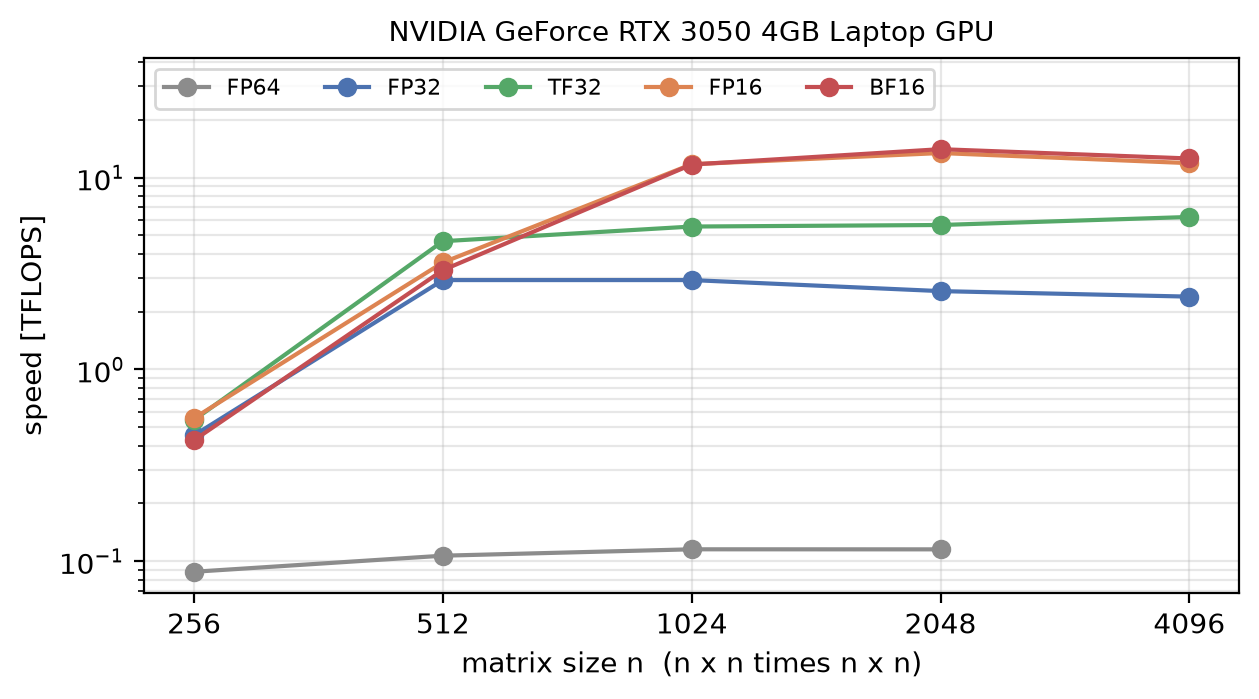
\includegraphics[width=0.74\textwidth]{figures/bench_matmul.png}

\small RTX 3050 노트북 GPU에서 잰 행렬곱 속도 (로그 눈금). 행렬이 작으면 GPU를 다 채우지 못해 느리다.
\end{minipage}
\end{center}

같은 곱을 FP64로 계산한 값을 기준으로 상대오차 $\|C-C_{\text{ref}}\|/\|C_{\text{ref}}\|$를 재면 ($n=1024$, 원소는 표준정규분포)

\begin{center}
{\small
\begin{tabular}{@{}lccl@{}}
\toprule
형식 & 최대 속도 (측정) & 상대오차 & 계산하는 장치 \\
\midrule
FP64 & $0.12$ TFLOPS & (기준) & CUDA core (FP64 회로가 적다) \\
FP32 & $2.9$ TFLOPS & $4.1\times10^{-7}$ & CUDA core \\
TF32 & $6.2$ TFLOPS & $2.9\times10^{-4}$ & tensor core \\
FP16 & $13.4$ TFLOPS & $3.6\times10^{-4}$ & tensor core \\
BF16 & $14.1$ TFLOPS & $3.1\times10^{-3}$ & tensor core \\
\bottomrule
\end{tabular}}
\end{center}

\begin{itemize}[leftmargin=1.5em]
\item tensor core를 쓰는 형식은 FP32보다 $2\sim5$배 빠르다. 대신 오차가 $10^{-7}$에서 $10^{-4}\sim10^{-3}$으로 커진다.
상대오차는 대략 가수의 비트 수로 정해진다 (FP32 $2^{-24}$, TF32와 FP16 $2^{-11}$, BF16 $2^{-8}$에 비례).
\item 신경망 학습은 이 정도 오차에 강하다. 딥러닝 노트 3.4절에서 \texttt{float16}으로 바꾸어도 예측이 하나도 바뀌지 않았던 것을 떠올리자.
\item \textbf{FP64는 FP32보다 약 $25$배 느리다.} GeForce (RTX) 계열은 FP64 회로를 일부러 적게 넣었다. 정밀도가 중요한 과학 계산 (유한요소법, 조건수가 큰 역문제)을 GPU로 할 때 주의해야 한다.
\end{itemize}

% =================================================
\section{성능을 재는 단위}\label{sec:metrics}
% =================================================

\subsection{FLOP, FLOPs, FLOPS}\label{sec:flops}

\begin{itemize}[leftmargin=1.5em]
\item \textbf{FLOP} (floating-point operation): 부동소수점수의 덧셈이나 곱셈 한 번. FMA $a\times b+c$는 $2$ FLOP으로 센다.
\item \textbf{FLOPs} (소문자 s): 연산의 \textbf{횟수}. ``이 모델은 이미지 한 장에 $4$ GFLOPs가 든다''처럼 쓴다.
\item \textbf{FLOPS} (대문자 S, FLOP per second): 초당 연산 횟수, 즉 \textbf{속도}.
\end{itemize}

\begin{center}
{\small
\begin{tabular}{@{}lll@{}}
\toprule
접두사 & 크기 & 예 \\
\midrule
GFLOPS (giga) & $10^{9}$ & 옛날 CPU \\
TFLOPS (tera) & $10^{12}$ & RTX 5090 FP32 약 $105$ TFLOPS \\
PFLOPS (peta) & $10^{15}$ & B200 BF16 약 $2.25$ PFLOPS \\
EFLOPS (exa) & $10^{18}$ & 최상위 슈퍼컴퓨터 \\
\bottomrule
\end{tabular}}
\end{center}

횟수를 속도로 나누면 시간이 나온다. $n\times n$ 행렬곱은 $2n^3$ FLOPs이므로 $n=8192$이면 약 $1.1\times10^{12}$ FLOPs이고,
$100$ TFLOPS인 GPU로 이론상 약 $0.011$초이다.

\subsection{Roofline model}\label{sec:roofline}

GPU는 ``VRAM에서 데이터 가져오기 $\to$ 계산하기 $\to$ 결과 쓰기''를 반복한다. 둘 중 \textbf{느린 쪽}이 속도를 정한다.
연산의 \textbf{산술 강도} (arithmetic intensity)를
\[
I = \frac{\text{연산 횟수 [FLOP]}}{\text{메모리에서 옮긴 양 [byte]}}
\]
로 정의하면, 도달할 수 있는 속도는
\[
\text{속도} \le \min\bigl(\text{최대 연산 성능},\; I\times\text{메모리 대역폭}\bigr) .
\]
이 식을 로그 눈금으로 그리면 비스듬한 선과 수평선으로 된 지붕 모양이 되어 \textbf{roofline model}이라고 부른다.

\begin{itemize}[leftmargin=1.5em]
\item \textbf{memory-bound}: $I$가 작은 연산. 데이터 하나를 가져와 계산을 조금만 한다. 대역폭이 속도를 정한다.
예: $y=2x+1$은 원소 하나에 $2$ FLOP, $8$ byte (읽기 $4$ + 쓰기 $4$)이므로 $I=0.25$. 활성화 함수, 정규화, 손실 계산이 여기에 속한다.
\item \textbf{compute-bound}: $I$가 큰 연산. 연산 성능이 속도를 정한다.
예: $n\times n$ 행렬곱은 $2n^3$ FLOP, $3n^2$개의 수를 옮기므로 $I=2n^3/(3n^2\cdot4)=n/6$ (FP32). $n=1024$이면 $I\approx170$이다.
\end{itemize}

\begin{center}
\begin{minipage}{\textwidth}\centering
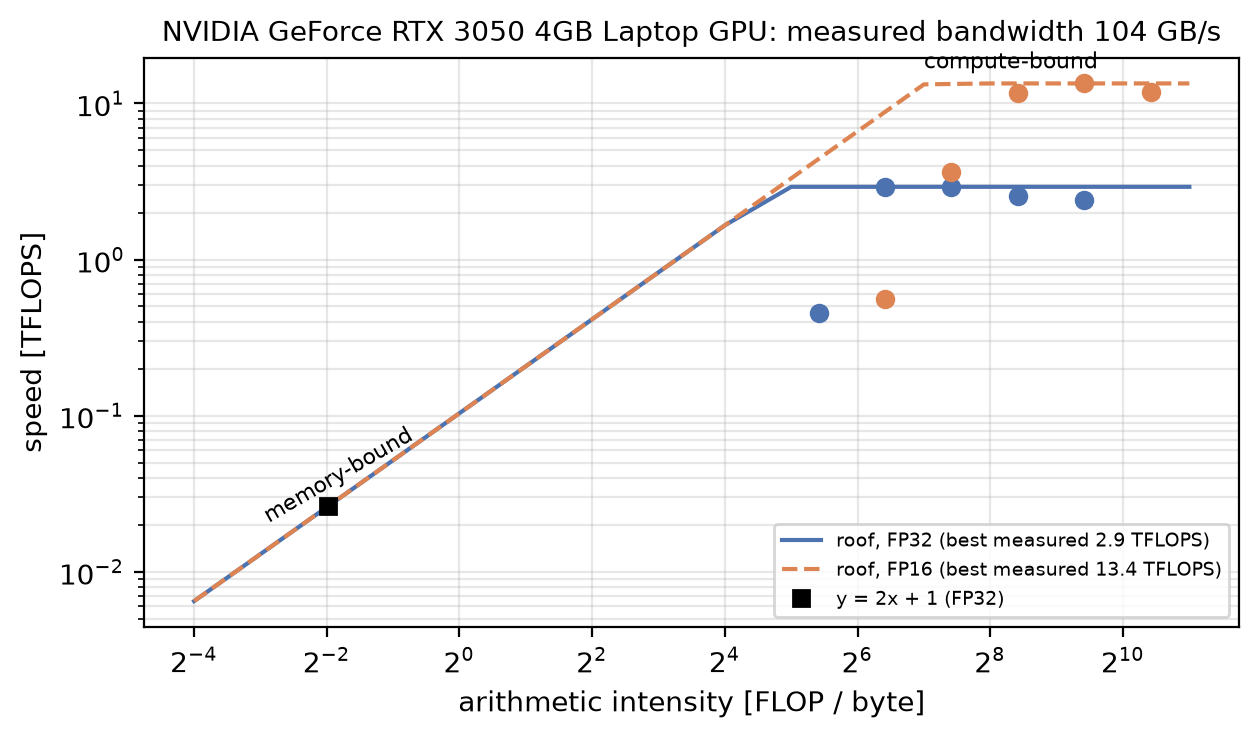
\includegraphics[width=0.74\textwidth]{figures/roofline_measured.png}

\small RTX 3050 노트북 GPU의 roofline. 측정한 VRAM 대역폭 ($104$ GB/s)과 측정한 최대 속도로 지붕을 그리고, 행렬곱 (점)과 $y=2x+1$ (검은 네모)을 표시하였다.
\end{minipage}
\end{center}

$y=2x+1$은 $26$ GFLOPS로 FP32 최대 속도의 $1\%$도 안 되지만, 대역폭은 다 쓰고 있다. 이 연산을 빠르게 하려면 GPU의 연산 성능이 아니라 \textbf{대역폭}이 커야 한다.
그래서 대역폭은 \textbf{메모리가 병목일 때만} 속도를 정한다. 대역폭이 크다고 무조건 학습이 빨라지는 것은 아니다.
PyTorch 2의 \texttt{torch.compile}은 원소별 연산 여러 개를 하나로 합쳐 (kernel fusion) 메모리 왕복을 줄이는 방법으로 memory-bound 연산을 빠르게 한다.

\subsection{사양표를 읽을 때 주의할 점}\label{sec:spec_reading}

\begin{itemize}[leftmargin=1.5em]
\item 사양표의 TFLOPS는 \textbf{이론상 최대값} (peak)이다. 실제 학습은 보통 그 $30\sim60\%$이다.
큰 모델 학습에서는 이 비율을 \textbf{MFU} (Model FLOPs Utilization)라고 부른다.
\item 같은 GPU라도 숫자 형식마다 TFLOPS가 크게 다르다. 항상 \textbf{어떤 형식 기준인지} 확인한다.
\item NVIDIA의 발표 자료에는 \textbf{with sparsity} 값이 함께 나오는 일이 많다. 행렬의 원소 $4$개 중 $2$개가 $0$인 특별한 경우에만 나오는 $2$배 값이므로, 보통의 학습에는 그 절반 (dense)을 보아야 한다.
\item 노트북 GPU는 같은 이름의 데스크톱 GPU보다 훨씬 느리다. 전력 한도 (강의자의 노트북은 $35$ W) 때문에 클럭이 낮다.
위의 측정에서 FP32 최대 속도가 $2.9$ TFLOPS로, CUDA core 수 ($20$ SM $\times128=2560$개)와 최대 클럭 ($2.1$ GHz)으로 계산한 $10.8$ TFLOPS보다 훨씬 낮은 이유이다.
\end{itemize}

% =================================================
\section{GPU의 세대와 종류}\label{sec:generations}
% =================================================

\subsection{아키텍처 이름}\label{sec:arch_names}

NVIDIA는 GPU의 설계 세대 (아키텍처, architecture)마다 과학자의 이름을 붙인다. 데이터센터 GPU의 이름 첫 글자가 아키텍처를 나타낸다.

\begin{center}
\begin{minipage}{\textwidth}\centering
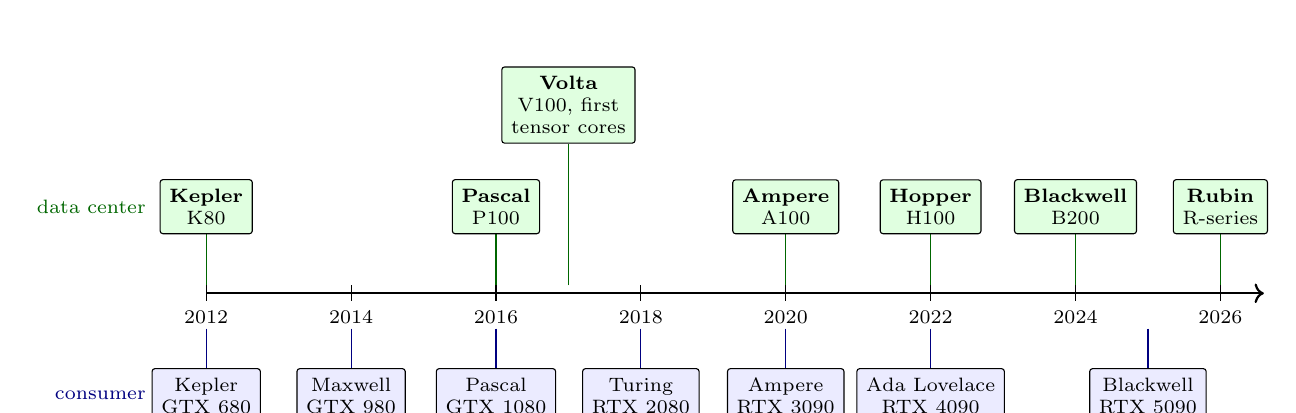
\begin{tikzpicture}[font=\scriptsize,x=0.92cm]
\draw[->,thick] (0,0) -- (14.6,0);
\foreach \yr in {2012,2014,...,2026} { \draw (\yr-2012,0.1) -- (\yr-2012,-0.1) node[below] {\yr}; }
\foreach \x/\name/\pr/\h in {0/Kepler/K80/0.75, 4/Pascal/P100/0.75, 5/Volta/{V100, first\\[0pt]tensor cores}/1.9, 8/Ampere/A100/0.75, 10/Hopper/H100/0.75, 12/Blackwell/B200/0.75, 14/Rubin/{R-series}/0.75} {
  \draw[green!40!black] (\x,0.1) -- (\x,\h);
  \node[draw,fill=green!12,rounded corners=1pt,align=center,anchor=south] at (\x,\h) {\textbf{\name}\\[0pt]\pr};
}
\foreach \x/\name/\pr in {0/Kepler/{GTX 680}, 2/Maxwell/{GTX 980}, 4/Pascal/{GTX 1080}, 6/Turing/{RTX 2080}, 8/Ampere/{RTX 3090}, 10/{Ada Lovelace}/{RTX 4090}, 13/Blackwell/{RTX 5090}} {
  \draw[blue!50!black] (\x,-0.45) -- (\x,-0.95);
  \node[draw,fill=blue!8,rounded corners=1pt,align=center,anchor=north] at (\x,-0.95) {\name\\[0pt]\pr};
}
\node[anchor=east,green!40!black] at (-0.7,1.1) {data center};
\node[anchor=east,blue!50!black] at (-0.7,-1.3) {consumer};
\end{tikzpicture}

\small NVIDIA GPU 아키텍처의 흐름. 위는 데이터센터용 (대표 제품), 아래는 소비자용 (GeForce). 연도는 대략적인 출시 시기이다.
\end{minipage}
\end{center}

\begin{center}
{\small
\begin{tabular}{@{}lll@{}}
\toprule
아키텍처 & 이름의 주인 & 대표 제품 \\
\midrule
Kepler & 요하네스 케플러, 천문학자 & K80 \\
Maxwell & 제임스 클러크 맥스웰, 물리학자 & GTX 980 \\
Pascal & 블레즈 파스칼, 수학자 & P100, GTX 1080 \\
Volta & 알레산드로 볼타, 물리학자 (전지) & V100 \\
Turing & 앨런 튜링, 수학자, 컴퓨터 과학자 & T4, RTX 20 \\
Ampere & 앙드레마리 앙페르, 물리학자 & A100, RTX 30 \\
Ada Lovelace & 에이다 러브레이스, 수학자 (최초의 프로그래머) & RTX 40 \\
Hopper & 그레이스 호퍼, 컴퓨터 과학자 (최초의 컴파일러, COBOL) & H100, H200 \\
Blackwell & 데이비드 블랙웰, 통계학자 (Rao--Blackwell 정리) & B200, RTX 50 \\
Rubin & 베라 루빈, 천문학자 (암흑물질의 증거) & 다음 세대 \\
\bottomrule
\end{tabular}}
\end{center}

\begin{center}
\photo{portrait_grace_hopper.jpg}{0.25\textwidth}{Grace Hopper (1906--1992)}\hspace{2em}
\photo{portrait_david_blackwell.jpg}{0.25\textwidth}{David Blackwell (1919--2010)}
\end{center}

\paragraph{제품 이름의 숫자와 글자.}
\begin{itemize}[leftmargin=1.5em]
\item \textbf{100}: 그 세대의 주력 데이터센터 제품 (V100, A100, H100).
\item \textbf{H200}: 같은 Hopper 칩에 HBM3e를 더 많이 ($141$ GB) 붙인 개량판.
\item \textbf{B200}: Blackwell은 \textbf{칩 두 개를 한 패키지에 묶어} 하나의 GPU처럼 쓴다.
\item \textbf{GB200}: Grace (NVIDIA의 ARM CPU)와 Blackwell GPU를 한 보드에 묶은 제품.
\item \textbf{RTX 5090}의 칩 이름은 GB202이다. G는 GeForce, B는 Blackwell. 즉 B200과 같은 세대의 설계로 만든 소비자용 제품이다.
\item \textbf{compute capability}: CUDA가 GPU의 기능을 구별하는 버전 번호이다. A100은 8.0, RTX 3050은 8.6, H100은 9.0, B200은 10.0, RTX 5090은 12.0이다.
PyTorch가 그 번호를 지원하도록 빌드되어 있어야 GPU를 쓸 수 있다 (8절).
\end{itemize}

\subsection{A100, H100, B200}\label{sec:a100_b200}

\begin{center}
{\small
\begin{tabular}{@{}lccc@{}}
\toprule
& A100 (2020) & H100 (2022) & B200 (2024) \\
\midrule
아키텍처, 공정 & Ampere, 7 nm & Hopper, 4 nm급 & Blackwell, 4 nm급 \\
트랜지스터 & $540$억 & $800$억 & $2{,}080$억 (칩 $2$개) \\
VRAM & $80$ GB HBM2e & $80$ GB HBM3 & $192$ GB HBM3e \\
메모리 대역폭 & $\sim$2.0 TB/s & $\sim$3.35 TB/s & $\sim$8 TB/s \\
BF16 tensor (dense) & $\sim$312 TFLOPS & $\sim$990 TFLOPS & $\sim$2,250 TFLOPS \\
새로 지원한 낮은 형식 & TF32, BF16 & FP8 & FP4 \\
FP64 & $9.7$ (tensor $19.5$) & $34$ (tensor $67$) & $\sim$40 TFLOPS \\
NVLink (GPU 하나) & $600$ GB/s & $900$ GB/s & $1{,}800$ GB/s \\
소비 전력 & $400$ W & $700$ W & $1{,}000$ W 이상 \\
\bottomrule
\end{tabular}}

\small 서버용 (SXM) 제품의 대략적인 발표 사양. 제품 구성에 따라 다르다.
\end{center}

세대가 바뀌며 달라진 것을 정리하면
\begin{enumerate}[label=(\arabic*)]
\item \textbf{더 낮은 정밀도로 더 많이 계산한다.} TF32 $\to$ FP8 $\to$ FP4. 발표 자료의 ``AI 성능 $n$배''는 정밀도를 낮춘 값끼리 비교한 경우가 많다. 같은 BF16으로 보면 세대마다 약 $2\sim3$배이다.
\item \textbf{메모리 용량과 대역폭이 커졌다.} 큰 언어 모델이 GPU에 들어가는가, 가중치를 얼마나 빨리 읽는가가 병목이 되었기 때문이다.
\item \textbf{칩 하나에서 여러 칩으로.} 칩 하나를 무한히 키울 수 없어서 (노광 장비의 최대 면적) B200은 칩 두 개를 붙였다. NVLink로 GPU 수십 개를 하나처럼 묶는다.
\item \textbf{전력이 크게 늘었다.} $400\to700\to1000$ W 이상. 수냉이 기본이 되어 가고 있다.
\item \textbf{FP64는 거의 정체되었다.} A100 $\to$ H100에서는 늘었지만 그 뒤로는 그대로이거나 오히려 줄었다. 데이터센터 GPU가 AI 전용 칩으로 바뀌고 있다.
\end{enumerate}

\begin{center}
\begin{minipage}{\textwidth}\centering
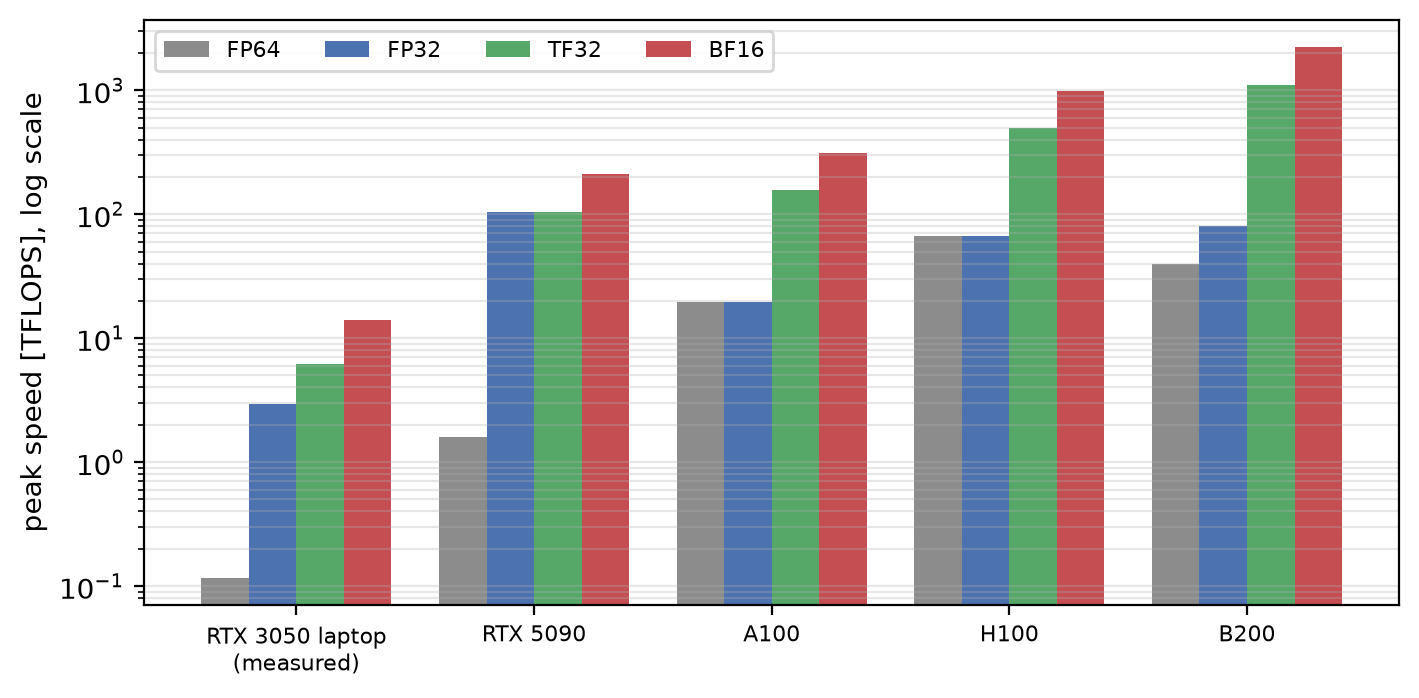
\includegraphics[width=0.84\textwidth]{figures/gpu_formats.png}

\small GPU와 숫자 형식에 따른 최대 행렬곱 속도 (로그 눈금, dense). RTX 3050은 측정값, 나머지는 발표 사양이다. A100과 H100의 FP64는 tensor core 값이다.
RTX 5090은 FP32는 A100보다 빠르지만 FP64는 훨씬 느리다.
\end{minipage}
\end{center}

\begin{center}
\photo{gpu_hgx_b200_sxm.jpg}{0.55\textwidth}{NVIDIA HGX B200 보드. B200 SXM 모듈 $8$개가 방열판 아래에 눕혀 꽂혀 있고, NVLink로 서로 연결된다.}\hspace{2em}
\photo{rack_dgx_gb200.jpg}{0.25\textwidth}{GPU 랙 (DGX GB200). 랙 하나에 GPU $72$개가 들어간다.}
\end{center}

\subsection{소비자용과 데이터센터용}\label{sec:consumer_dc}

\begin{center}
{\small
\begin{tabular}{@{}lll@{}}
\toprule
& 소비자용 (RTX 5090) & 데이터센터용 (H100) \\
\midrule
VRAM & $32$ GB GDDR7 & $80$ GB HBM3 \\
메모리 대역폭 & $1.8$ TB/s & $3.35$ TB/s \\
FP32 (CUDA core) & $\sim$105 TFLOPS & $\sim$67 TFLOPS \\
BF16 tensor & $\sim$210 TFLOPS & $\sim$990 TFLOPS \\
FP64 & $\sim$1.6 TFLOPS ($=$FP32의 $1/64$) & $34\sim67$ TFLOPS \\
GPU 사이의 연결 & PCIe만 (NVLink 없음) & NVLink $900$ GB/s \\
ECC 메모리 & 없음 & 있음 \\
모양 & PCIe 카드, 팬 냉각 & SXM 모듈, 서버 냉각 \\
가격 & 수백만 원 & 수천만 원 \\
\bottomrule
\end{tabular}}
\end{center}

\begin{itemize}[leftmargin=1.5em]
\item 보통의 FP32 계산만 보면 RTX 5090이 오히려 빠르다. 데이터센터 GPU의 강점은 용량, 대역폭, tensor core, NVLink, FP64이다.
\item \textbf{ECC} (Error-Correcting Code): 메모리의 비트가 우연히 바뀌면 (우주선 등) 찾아서 고치는 기능. 수천 GPU로 몇 주씩 학습할 때 중요하다.
\item 연구실의 작은 모델 연구나 GPU마다 다른 실험을 돌리는 용도에는 소비자용이 가격 대비 좋다. FP64가 핵심인 계산에는 맞지 않는다.
\end{itemize}

\subsection{GPU 여러 장}\label{sec:multigpu}

데이터 병렬 학습 (딥러닝 노트 3.3절)에서는 매 step마다 GPU들이 기울기를 평균한다. 이 통신이 어떤 통로로 가는지가 중요하다.

\begin{center}
\begin{minipage}{\textwidth}\centering
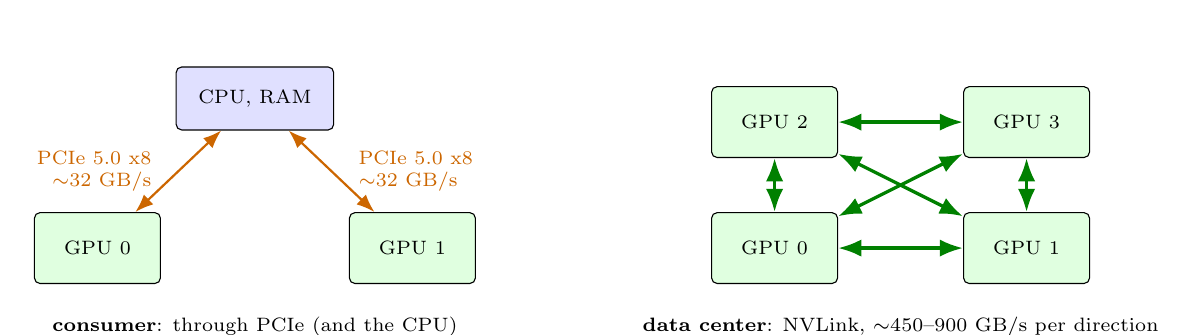
\begin{tikzpicture}[>=Latex,font=\scriptsize,
  g/.style={draw,fill=green!12,rounded corners=2pt,minimum width=16mm,minimum height=9mm,align=center}]
\begin{scope}
\node[draw,fill=blue!12,rounded corners=2pt,minimum width=20mm,minimum height=8mm] (cpu) at (2.0,1.9) {CPU, RAM};
\node[g] (a) at (0,0) {GPU 0}; \node[g] (b) at (4.0,0) {GPU 1};
\draw[<->,thick,orange!80!black] (a) -- node[left=6pt,align=right] {PCIe 5.0 x8\\$\sim$32 GB/s} (cpu);
\draw[<->,thick,orange!80!black] (b) -- node[right=6pt,align=left] {PCIe 5.0 x8\\$\sim$32 GB/s} (cpu);
\node at (2.0,-1.0) {\textbf{consumer}: through PCIe (and the CPU)};
\end{scope}
\begin{scope}[xshift=8.6cm]
\node[g] (c) at (0,0) {GPU 0}; \node[g] (d) at (3.2,0) {GPU 1};
\node[g] (e) at (0,1.6) {GPU 2}; \node[g] (f) at (3.2,1.6) {GPU 3};
\foreach \u/\v in {c/d,e/f,c/e,d/f,c/f,d/e} \draw[<->,very thick,green!50!black] (\u) -- (\v);
\node at (1.6,-1.0) {\textbf{data center}: NVLink, $\sim$450--900 GB/s per direction};
\end{scope}
\end{tikzpicture}

\small GPU 사이의 통신. 소비자용 GPU는 PCIe로, 데이터센터용 GPU는 NVLink로 직접 주고받는다.
\end{minipage}
\end{center}

\begin{itemize}[leftmargin=1.5em]
\item \textbf{NVLink}: NVIDIA GPU끼리 직접 잇는 전용 고속 연결. RTX 40 이후의 소비자용 GPU에는 없다.
\item \textbf{P2P} (peer-to-peer): GPU가 CPU 메모리를 거치지 않고 다른 GPU의 메모리를 직접 읽는 기능. GeForce에서는 보통 막혀 있다.
\item \textbf{NCCL} (NVIDIA Collective Communications Library, ``니클''): 여러 GPU 사이에 기울기를 평균하는 (all-reduce) 통신 라이브러리. PyTorch의 \texttt{DistributedDataParallel} (DDP)이 이것을 쓴다.
\item 모델이 작으면 기울기의 양이 적어서 PCIe로도 충분하다. 연구에서는 GPU마다 \textbf{다른 실험} (다른 seed, 다른 설정)을 하나씩 돌리는 것이 가장 흔하고, 이때는 통신이 전혀 없다.
\end{itemize}

\begin{lstlisting}[numbers=none]
# two independent experiments, one per GPU (Linux shell)
CUDA_VISIBLE_DEVICES=0 python train.py --seed 1 &
CUDA_VISIBLE_DEVICES=1 python train.py --seed 2 &

# one experiment on both GPUs with DDP
torchrun --nproc_per_node=2 train_ddp.py
\end{lstlisting}

% =================================================
\section{소프트웨어 스택}\label{sec:software}
% =================================================

\textbf{CUDA} (Compute Unified Device Architecture)는 NVIDIA가 2007년에 내놓은 \textbf{GPU로 일반 계산을 하기 위한 플랫폼}이다.
그 전에는 GPU로 과학 계산을 하려면 행렬을 그림 (texture)으로, 계산을 픽셀 칠하기로 위장해야 했다.
CUDA라는 이름은 여러 가지를 함께 가리킨다.

\begin{center}
\begin{minipage}{\textwidth}\centering
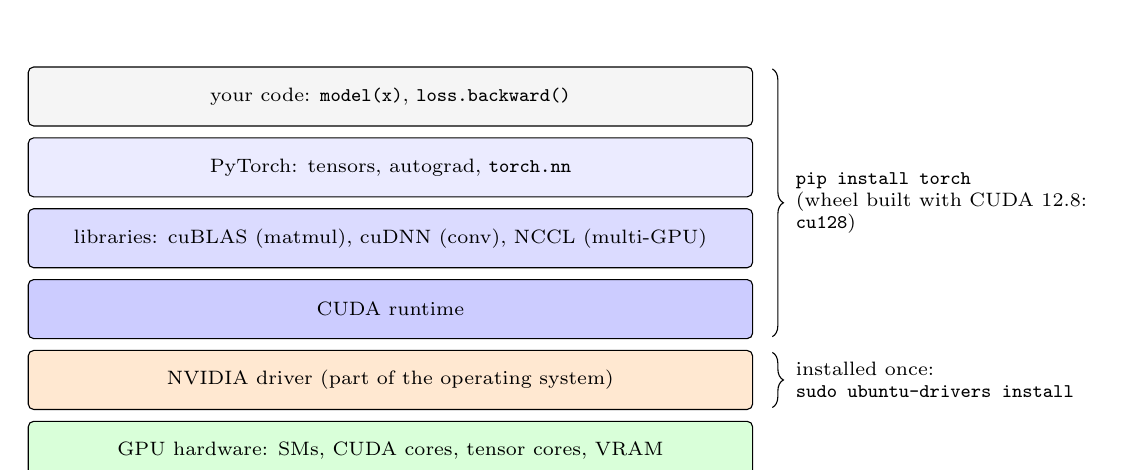
\begin{tikzpicture}[font=\scriptsize,
  layer/.style={draw,rounded corners=2pt,minimum width=92mm,minimum height=7.5mm,align=center}]
\node[layer,fill=black!4] (l1) at (0,4.0) {your code: \texttt{model(x)}, \texttt{loss.backward()}};
\node[layer,fill=blue!8] (l2) at (0,3.1) {PyTorch: tensors, autograd, \texttt{torch.nn}};
\node[layer,fill=blue!14] (l3) at (0,2.2) {libraries: cuBLAS (matmul), cuDNN (conv), NCCL (multi-GPU)};
\node[layer,fill=blue!20] (l4) at (0,1.3) {CUDA runtime};
\node[layer,fill=orange!18] (l5) at (0,0.4) {NVIDIA driver (part of the operating system)};
\node[layer,fill=green!15] (l6) at (0,-0.5) {GPU hardware: SMs, CUDA cores, tensor cores, VRAM};
\draw[decorate,decoration={brace,amplitude=4pt}] (4.85,4.35) -- (4.85,0.95)
  node[midway,right=5pt,align=left] {\texttt{pip install torch}\\(wheel built with CUDA 12.8:\\\texttt{cu128})};
\draw[decorate,decoration={brace,amplitude=4pt}] (4.85,0.75) -- (4.85,0.05)
  node[midway,right=5pt,align=left] {installed once:\\\texttt{sudo ubuntu-drivers install}};
\end{tikzpicture}

\small PyTorch로 학습할 때의 소프트웨어 층. PyTorch 패키지가 CUDA 라이브러리를 함께 가지고 오므로, 드라이버만 따로 설치하면 된다.
\end{minipage}
\end{center}

\begin{itemize}[leftmargin=1.5em]
\item \textbf{드라이버} (driver): 운영체제가 GPU를 다루게 하는 프로그램. GPU 세대가 새로우면 새 드라이버가 필요하다 (RTX 5090은 570 버전 이상).
\item \textbf{CUDA Toolkit}: 컴파일러 \texttt{nvcc}와 라이브러리를 묶은 개발 패키지. GPU 코드를 직접 짤 때만 따로 설치하면 된다.
\item \textbf{cuBLAS} (CUDA Basic Linear Algebra Subprograms): 행렬곱 라이브러리. \textbf{cuDNN} (CUDA Deep Neural Network library): 합성곱 등 신경망 연산 라이브러리.
\item \textbf{PyTorch의 \texttt{cu128}}: CUDA 12.8로 빌드한 PyTorch라는 뜻이다. RTX 5090 (compute capability 12.0)을 쓰려면 \texttt{cu128} 이상으로 빌드된 PyTorch가 필요하다.
\item \texttt{nvidia-smi}에 나오는 ``CUDA Version''은 설치된 Toolkit의 버전이 아니라 \textbf{그 드라이버가 실행할 수 있는 가장 높은 CUDA 버전}이다.
\item PyTorch에서 \texttt{device="cuda"}, \texttt{torch.cuda}는 ``NVIDIA GPU''를 가리키는 이름이다. AMD GPU의 대응 플랫폼은 ROCm이다.
\end{itemize}

\texttt{device\_info.py}를 실행하면 내 컴퓨터의 상태를 확인할 수 있다. 강의자의 노트북에서는

\begin{lstlisting}[numbers=none,language={}]
PyTorch         : 2.5.1+cu121
CUDA (PyTorch)  : 12.1
GPU 0           : NVIDIA GeForce RTX 3050 4GB Laptop GPU
  VRAM          : 4.0 GiB
  SMs           : 20
  compute cap.  : 8.6   (sm_86)
matmul allow_tf32 : False
cudnn  allow_tf32 : True
\end{lstlisting}

% =================================================
\section{개발 환경}\label{sec:devenv}
% =================================================

GPU 컴퓨터는 보통 \textbf{Linux} (주로 Ubuntu)를 설치하고, 다른 컴퓨터에서 접속하여 쓴다.
GPU 드라이버, CUDA, PyTorch가 Linux를 가장 먼저 지원하고, 서버는 화면 없이 원격으로 쓰는 것이 일반적이기 때문이다.

\begin{center}
\begin{minipage}{\textwidth}\centering
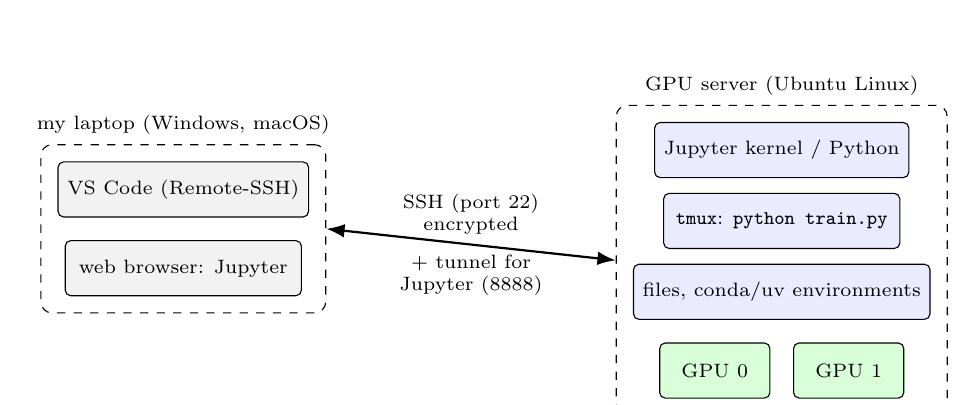
\begin{tikzpicture}[>=Latex,font=\scriptsize,
  b/.style={draw,rounded corners=2pt,minimum width=30mm,minimum height=7mm,align=center}]
\node[b,fill=black!5] (vs) at (0,1.0) {VS Code (Remote-SSH)};
\node[b,fill=black!5] (br) at (0,0) {web browser: Jupyter};
\node[draw,dashed,rounded corners=4pt,fit=(vs)(br),inner sep=6pt,label={[font=\scriptsize]above:my laptop (Windows, macOS)}] (lap) {};
\node[b,fill=blue!8] (k) at (7.6,1.5) {Jupyter kernel / Python};
\node[b,fill=blue!8] (t) at (7.6,0.6) {\texttt{tmux}: \texttt{python train.py}};
\node[b,fill=blue!8] (f) at (7.6,-0.3) {files, conda/uv environments};
\node[b,fill=green!15,minimum width=14mm] (g0) at (6.75,-1.3) {GPU 0};
\node[b,fill=green!15,minimum width=14mm] (g1) at (8.45,-1.3) {GPU 1};
\node[draw,dashed,rounded corners=4pt,fit=(k)(t)(f)(g0)(g1),inner sep=6pt,label={[font=\scriptsize]above:GPU server (Ubuntu Linux)}] (srv) {};
\draw[<->,thick] (lap.east) -- node[above,align=center] {SSH (port 22)\\encrypted} node[below,align=center] {+ tunnel for\\Jupyter (8888)} (srv.west);
\end{tikzpicture}

\small 원격 개발 환경. 계산과 파일은 서버에 있고, 내 컴퓨터는 화면만 보여 준다.
\end{minipage}
\end{center}

\begin{itemize}[leftmargin=1.5em]
\item \textbf{SSH} (Secure Shell): 다른 컴퓨터에 암호화된 연결로 접속하여 명령을 실행하는 방법. 비밀번호 대신 SSH 키를 쓰는 것이 안전하다.
\item \textbf{VS Code Remote-SSH}: 내 컴퓨터의 VS Code로 서버의 파일을 편집하고, 서버의 터미널과 Python을 쓴다.
\item \textbf{Jupyter notebook}: 코드를 \textbf{셀} 단위로 실행하고 결과와 그림이 셀 아래에 남는, 브라우저 기반의 대화형 실행 환경이다.
코드를 실행하는 쪽 (\textbf{kernel})이 서버에 있으면 계산과 파일은 모두 서버에서 일어난다.
kernel의 작업 폴더는 기본으로 노트북 파일이 있는 폴더이다. 노트북에서 \texttt{.py} 모듈을 \texttt{import}하여 쓸 수 있고, \texttt{\%autoreload 2}를 켜 두면 고친 모듈을 자동으로 다시 읽는다.
VS Code에서도 \texttt{.ipynb}를 열어 같은 kernel로 실행할 수 있다.
\item \textbf{tmux} (terminal multiplexer): SSH 연결이 끊겨도 서버에서 프로그램이 계속 돌게 하는 터미널 관리 프로그램. 몇 시간씩 걸리는 학습은 노트북이 아니라 \texttt{tmux} 안의 \texttt{.py} 스크립트로 돌린다.
\item \textbf{가상환경} (virtual environment): 프로젝트마다 Python 패키지를 따로 설치하는 공간. \texttt{conda}, \texttt{uv}, \texttt{venv} 등을 쓴다. 운영체제의 Python에 직접 설치하지 않는다.
\item \textbf{모니터링}: \texttt{nvidia-smi} (사용률, VRAM, 온도, 전력), \texttt{nvtop} (실시간 그래프).
\end{itemize}

\begin{lstlisting}[numbers=none]
# on the server: start Jupyter without a browser
jupyter lab --no-browser --port=8888
# on my laptop: forward port 8888 through SSH, then open http://localhost:8888
ssh -L 8888:localhost:8888 myserver
\end{lstlisting}

% =================================================
\section{사례: 연구용 GPU 워크스테이션}\label{sec:case}
% =================================================

지금까지의 내용을 한 번에 써 보자. 다음은 RTX 5090 두 장을 학습용으로 쓰는 연구용 워크스테이션을 맞출 때 검토한 사항이다.

\begin{center}
{\small
\begin{tabular}{@{}>{\raggedright\arraybackslash}p{24mm}>{\raggedright\arraybackslash}p{48mm}>{\raggedright\arraybackslash}p{78mm}@{}}
\toprule
부품 & 구성 & 확인한 것 \\
\midrule
GPU & RTX 5090 $\times$ 2 & 처음 1장, 나중에 1장 추가. 카드 두께 (아래 그림) \\
CPU & Ryzen 9 (16코어, 내장 그래픽 있음) & 학습은 GPU가 하므로 CPU는 데이터 준비에 충분하면 된다 \\
메인보드 & X870E 칩셋 & 두 번째 슬롯이 \textbf{CPU 직결 x8}인가 (보급형은 칩셋 경유 x4) \\
메모리 & DDR5-5600 64 GB $\times$ 2 & VRAM 합계 ($64$ GB)의 $2$배. $4$장을 꽂으면 보장 속도가 3600으로 내려가서 $2$장으로 \\
SSD & NVMe 4 TB & M.2\_1 (CPU 직결)에. GPU 2와 lane을 나누는 M.2\_2, M.2\_3은 비운다 \\
파워 & 2000 W & GPU $575\times2$ + CPU $270$ + 나머지 $\approx1{,}530$ W \\
케이스 & 확장 슬롯 9개 & 두 번째 카드가 메인보드 아래로 내려온다 \\
\bottomrule
\end{tabular}}
\end{center}

\paragraph{카드 사이의 틈.}
두 x16 슬롯의 간격이 약 $81$ mm ($4$슬롯)이고, 그래픽카드는 슬롯에서 아래쪽으로 두껍게 자리를 차지한다.
그래서 위 카드와 아래 카드 사이의 틈은 대략 ``슬롯 간격 $-$ \textbf{위쪽} 카드의 두께''이다.

\begin{center}
\begin{minipage}{\textwidth}\centering
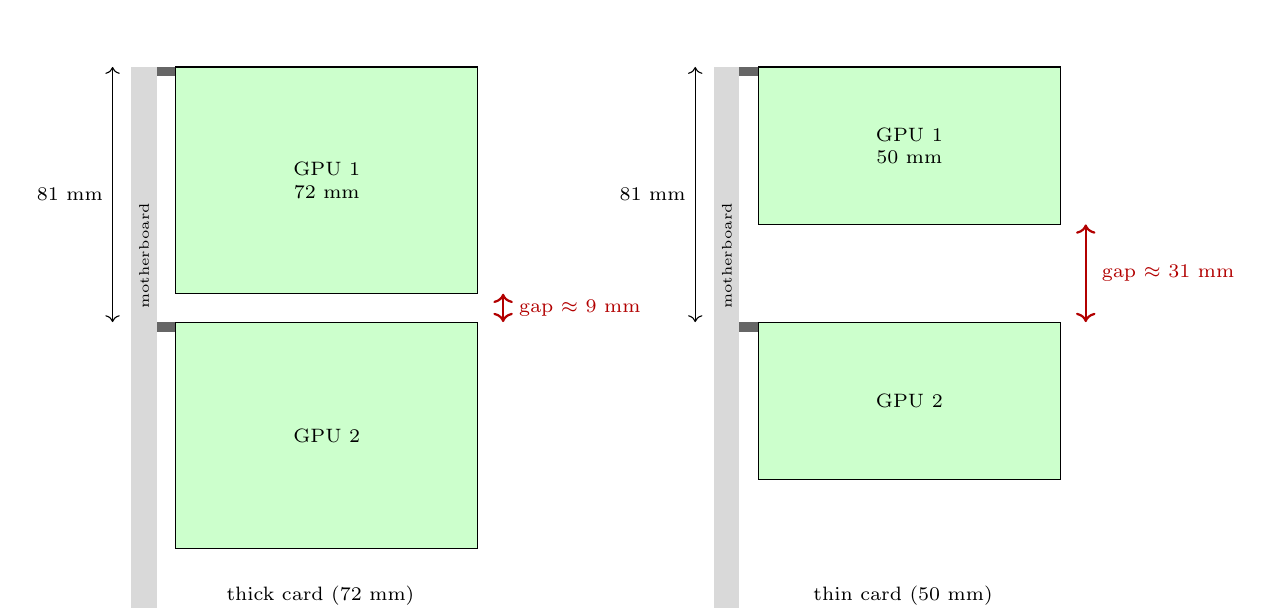
\begin{tikzpicture}[font=\scriptsize,x=0.4mm,y=0.4mm]
\foreach \ox/\t/\name in {0/72/{thick card (72 mm)}, 185/50/{thin card (50 mm)}} {
  \begin{scope}[xshift=\ox*0.4mm]
  \fill[black!15] (0,0) rectangle (8,-175);
  \node[rotate=90,font=\tiny] at (4,-60) {motherboard};
  \foreach \s in {0,81} { \fill[black!60] (8,-\s) rectangle (14,-\s-3); }
  \draw[fill=green!20] (14,0) rectangle (110,-\t) node[pos=0.5,align=center] {GPU 1\\\t\ mm};
  \draw[fill=green!20] (14,-81) rectangle (110,-81-\t) node[pos=0.5,align=center] {GPU 2};
  \draw[<->,red!70!black,thick] (118,-\t) -- (118,-81);
  \pgfmathtruncatemacro{\gap}{81-\t}
  \node[anchor=west,red!70!black] at (120,-\t/2-81/2) {gap $\approx$ \gap\ mm};
  \draw[<->] (-6,0) -- (-6,-81) node[midway,left] {81 mm};
  \node at (60,-168) {\name};
  \end{scope}
}
\end{tikzpicture}

\small 슬롯 간격이 같을 때 카드 두께에 따른 틈 (옆에서 본 모습). 위쪽 카드가 두꺼우면 아래 카드를 얇은 것으로 바꾸어도 틈은 그대로이다.
\end{minipage}
\end{center}

틈이 $10$ mm 정도로 좁으면 위쪽 카드의 팬이 아래 카드의 뜨거운 공기를 빨아들여, 장시간 학습에서 클럭이 떨어진다.
GPU의 전력 한도를 낮추면 (\texttt{sudo nvidia-smi -pl 450}) 성능은 몇 \% 줄지만 발열과 소음이 크게 준다.

\begin{center}
\photo{power_12vhpwr_adapter.jpg}{0.47\textwidth}{16핀 GPU 전원 커넥터 (12VHPWR, 지금은 12V-2x6). 8핀 $4$개를 하나로 모은 변환 케이블이다. 끝까지 꽂아야 한다.}\hfill
\photo{sli_bridge_gtx1080.jpg}{0.47\textwidth}{그래픽카드 두 장을 잇는 SLI 브리지 (GTX 1080). NVLink 브리지도 이렇게 생겼다. 최신 소비자용 GPU에는 없다.}\\[0.8em]
\photo{cooler_aio_360.jpg}{0.47\textwidth}{일체형 수냉 CPU 냉각기 (펌프, 호스, 360 mm 라디에이터)}\hfill
\photo{cooler_tower_nh_d15.jpg}{0.47\textwidth}{공랭 CPU 냉각기 (타워 두 개, 팬 두 개)}
\end{center}

\begin{thinkbox}[확인 목록]
\begin{itemize}[leftmargin=1.5em]
\item 두 번째 GPU 슬롯이 CPU 직결 x8인가? 그 슬롯과 lane을 나누는 M.2 슬롯은 어디인가?
\item 카드 두께와 슬롯 간격으로 계산한 틈, 케이스의 슬롯 수, 아래 카드 아래의 공간
\item 파워 용량, GPU마다 따로 연결하는 전원 케이블
\item CPU가 메인보드의 BIOS 버전에서 지원되는가 (새 CPU는 BIOS 업데이트가 필요할 수 있다)
\item 모니터는 CPU 내장 그래픽 (메인보드의 포트)에 연결하면 두 GPU를 모두 계산 전용으로 쓸 수 있다
\item 드라이버 버전과 PyTorch 빌드 (\texttt{cu128} 이상)가 GPU의 세대를 지원하는가
\end{itemize}
\end{thinkbox}

% =================================================
\section{용어 정리}\label{sec:glossary}
% =================================================

{\small
\begin{longtable}{@{}>{\raggedright\arraybackslash}p{24mm}>{\raggedright\arraybackslash}p{50mm}>{\raggedright\arraybackslash}p{76mm}@{}}
\toprule
용어 & 원어 & 뜻 \\
\midrule
\endfirsthead
\toprule
용어 & 원어 & 뜻 \\
\midrule
\endhead
\bottomrule
\endfoot
\multicolumn{3}{@{}l}{\textbf{부품}} \\
CPU & Central Processing Unit & 중앙 처리 장치. 프로그램 전체를 지휘한다 \\
GPU & Graphics Processing Unit & 그래픽 처리 장치. 대량의 단순 계산을 동시에 한다 \\
PSU & Power Supply Unit & 파워 서플라이. 전기를 공급한다 \\
SSD & Solid State Drive & 반도체 (NAND flash) 저장장치 \\
HDD & Hard Disk Drive & 회전하는 자기 원판에 저장하는 장치 \\
volatile, non-volatile & 휘발성, 비휘발성 & 전원이 꺼지면 사라지는 (RAM), 남는 (SSD, HDD) 저장 \\
NAND flash & NAND: NOT AND 게이트 & 셀을 직렬로 이은 flash. SSD의 저장 매체 \\
NOR flash & NOR: NOT OR 게이트 & 셀을 따로 연결한 flash. BIOS 등 작은 펌웨어 저장 \\
flash & & 블록 단위로 한꺼번에 지우는 비휘발성 메모리 (카메라 플래시에서 온 이름) \\
garbage collection & & SSD가 쓸모없어진 페이지가 많은 블록을 모아 지우는 정리 작업 \\
TRIM & & 지워도 되는 데이터를 운영체제가 SSD에 알려 주는 명령 \\
SLC, MLC, TLC, QLC & Single/Multi/Triple/Quad-Level Cell & NAND 셀 하나에 $1$, $2$, $3$, $4$비트를 저장하는 방식 \\
seek & & HDD의 헤드를 원하는 트랙으로 옮기는 동작 (수 ms) \\
IOPS & Input/Output Operations Per Second & 초당 처리하는 작은 읽기·쓰기의 횟수 \\
TBW & TeraBytes Written & SSD가 수명 동안 쓸 수 있는 양 \\
page cache & & 운영체제가 한 번 읽은 파일을 RAM에 보관해 두는 것 \\
BIOS & Basic Input/Output System & 전원을 켤 때 부품을 점검하고 운영체제를 부르는 메인보드의 프로그램 \\
iGPU & integrated GPU & CPU 안의 내장 그래픽. 화면 출력용 \\
\multicolumn{3}{@{}l}{\textbf{연결}} \\
PCIe & PCI Express (Peripheral Component Interconnect Express) & 메인보드 안의 고속 직렬 연결 규격 \\
lane & & PCIe 통로의 단위. x16은 lane $16$개 \\
chipset & & CPU와 여러 장치를 잇는 메인보드의 중계 칩 \\
bus & (라틴어 omnibus, ``모두를 위한'') & 여러 부품이 데이터를 주고받는 공용 전선 묶음 \\
pin & 핀 & 칩, 소켓, 커넥터의 금속 접점 하나. 전선 하나가 핀 하나에 닿는다 \\
width & 폭 & 동시에 보내는 비트 수 (데이터선의 가닥 수). 대역폭 $=$ 폭 $\times$ 핀당 속도 $\div8$ \\
serial, parallel & 직렬, 병렬 & 비트를 한 줄로 차례로 보내는 방식과 여러 선으로 동시에 보내는 방식 \\
memory bus & & CPU (메모리 컨트롤러)와 메모리 사이의 전용 병렬 버스. PCIe가 아니다 \\
channel & memory channel & 메모리 컨트롤러가 따로 다루는 메모리 버스 하나 ($64$비트) \\
IMC & Integrated Memory Controller & CPU 안의 메모리 컨트롤러 \\
CXL & Compute Express Link & PCIe와 같은 선로로 메모리 등을 연결하는 규격 \\
M.2 & & SSD 등을 꽂는 작은 슬롯의 모양 규격 \\
NVMe & Non-Volatile Memory Express & PCIe를 쓰는 SSD 통신 규격 \\
ATA & AT Attachment (AT: IBM PC/AT, Advanced Technology) & 1984년 IBM PC/AT에서 온 하드디스크 연결 방식 \\
IDE, PATA & Integrated Drive Electronics, Parallel ATA & 넓은 리본 케이블로 병렬 전송하던 옛 ATA \\
SATA & Serial ATA & ATA를 직렬로 바꾼 저장장치 연결 규격. 최대 약 $0.55$ GB/s \\
NVLink & & NVIDIA GPU끼리 잇는 전용 고속 연결 \\
P2P & peer-to-peer & GPU가 다른 GPU의 메모리를 직접 읽는 기능 \\
SXM & (Server PCI Express Module) & 데이터센터 GPU를 서버 보드에 꽂는 모듈 형태 \\
\multicolumn{3}{@{}l}{\textbf{메모리}} \\
RAM & Random Access Memory & 임의 접근 메모리. 어느 주소든 바로 읽고 쓴다 \\
DRAM & Dynamic RAM & 축전기에 저장하여 refresh가 필요한 RAM. 메인 메모리, VRAM \\
SRAM & Static RAM & 트랜지스터 회로에 저장하는 빠른 RAM. 캐시 \\
SDRAM & Synchronous DRAM & 시스템 클럭에 맞추어 동작하는 DRAM \\
DDR & Double Data Rate & 클럭의 양쪽 가장자리에서 전송하는 SDRAM. DDR5는 $5$세대 \\
GDDR & Graphics DDR & 그래픽카드용 DDR. 세대 번호는 DDR과 따로 간다 \\
HBM & High Bandwidth Memory & DRAM을 쌓아 GPU 옆에 붙인 고대역폭 메모리 \\
HBM3E & HBM 3rd generation, Extended & HBM3의 개량판 \\
LPDDR & Low Power DDR & 휴대폰, 노트북용 저전력 DDR \\
DIMM & Dual In-line Memory Module & 메모리 칩을 붙인 막대 모양의 모듈. 양면 접점이 서로 다른 신호를 나른다 \\
SO-DIMM & Small Outline DIMM & 노트북용 작은 DIMM \\
VRAM & Video RAM & GPU 전용 메모리 \\
ECC & Error-Correcting Code & 메모리 오류를 찾아 고치는 기능 \\
TSV & Through-Silicon Via & 실리콘을 관통하는 수직 배선. HBM의 층을 잇는다 \\
JEDEC & Joint Electron Device Engineering Council & 반도체 메모리 표준 단체 \\
MT/s & mega-transfers per second & 초당 백만 번 전송. DDR5-5600 $=5600$ MT/s \\
cache & & 프로세서 안의 작고 빠른 메모리 (L1, L2) \\
bandwidth & 대역폭 & 초당 옮길 수 있는 데이터의 양 (GB/s) \\
latency & 지연시간 & 요청 후 첫 데이터가 오기까지의 시간 (ns) \\
pinned memory & page-locked memory & 운영체제가 옮기지 않는 고정 메모리. GPU로 빨리 복사된다 \\
\multicolumn{3}{@{}l}{\textbf{GPU의 내부}} \\
SM & Streaming Multiprocessor & GPU를 이루는 기본 블록. CPU의 코어에 해당 \\
CUDA core & & SM 안의 FP32 계산기 한 칸 \\
tensor core & & 작은 행렬곱을 한 번에 하는 전용 회로 \\
warp & & 같은 명령을 함께 실행하는 thread $32$개의 묶음 \\
SIMT & Single Instruction, Multiple Threads & 한 명령을 여러 thread가 다른 데이터에 동시에 실행하는 방식 \\
FMA & Fused Multiply-Add & $a\times b+c$를 한 번에 계산하는 연산 ($2$ FLOP) \\
die & & 웨이퍼에서 잘라 낸 칩 한 조각 \\
throttling & & 온도나 전력 때문에 클럭을 스스로 낮추는 것 \\
\multicolumn{3}{@{}l}{\textbf{숫자 형식}} \\
FP64, FP32, FP16 & Floating Point, $64$/$32$/$16$ bits & 배정밀도, 단정밀도, 반정밀도 부동소수점수 \\
TF32 & TensorFloat-32 & tensor core용 $19$비트 계산 형식 (지수 $8$, 가수 $10$) \\
BF16 & brain floating point 16 & 지수 $8$, 가수 $7$의 $16$비트 형식 \\
FP8, FP4 & & $8$비트, $4$비트 부동소수점수 (E4M3, E5M2, E2M1) \\
mixed precision & 혼합 정밀도 & 매개변수는 FP32로 두고 계산은 16비트로 하는 학습 \\
\multicolumn{3}{@{}l}{\textbf{성능}} \\
FLOP & floating-point operation & 부동소수점 연산 한 번 \\
FLOPs & & 연산 횟수 \\
FLOPS & FLOP per second & 초당 연산 횟수. TFLOPS $=10^{12}$ FLOPS \\
arithmetic intensity & 산술 강도 & 옮긴 바이트 하나당 연산 횟수 \\
roofline model & & 최대 연산 성능과 대역폭으로 속도의 상한을 그린 그래프 \\
memory-bound & & 대역폭이 속도를 정하는 상태 \\
compute-bound & & 연산 성능이 속도를 정하는 상태 \\
MFU & Model FLOPs Utilization & 실제 학습 속도 / 최대 연산 성능 \\
dense, sparsity & & sparsity는 원소 절반이 $0$인 행렬에서만 나오는 $2$배 성능 값 \\
TGP, TDP & Total Graphics Power, Thermal Design Power & 그래픽카드 전체, CPU의 설계 전력 \\
\multicolumn{3}{@{}l}{\textbf{소프트웨어}} \\
CUDA & Compute Unified Device Architecture & NVIDIA GPU로 일반 계산을 하는 플랫폼 \\
cuBLAS & CUDA Basic Linear Algebra Subprograms & 행렬곱 등 선형대수 라이브러리 \\
cuDNN & CUDA Deep Neural Network library & 합성곱 등 신경망 연산 라이브러리 \\
NCCL & NVIDIA Collective Communications Library & GPU 사이의 통신 (all-reduce) 라이브러리 \\
DDP & DistributedDataParallel & PyTorch의 데이터 병렬 학습 \\
FSDP & Fully Sharded Data Parallel & 매개변수까지 GPU들에 나누어 두는 데이터 병렬 \\
compute capability & & CUDA가 GPU 세대를 구별하는 버전 번호 (예: 8.6, 12.0) \\
ROCm & (Radeon Open Compute) & AMD GPU의 계산 플랫폼 \\
\multicolumn{3}{@{}l}{\textbf{개발 환경}} \\
SSH & Secure Shell & 암호화된 원격 접속 \\
tmux & terminal multiplexer & 접속이 끊겨도 프로그램이 계속 도는 터미널 관리 \\
kernel (Jupyter) & & 노트북의 코드를 실제로 실행하는 프로세스 \\
nvidia-smi & NVIDIA System Management Interface & GPU 상태를 보는 명령 \\
\end{longtable}}

% =================================================
\section{정리}\label{sec:summary}
% =================================================

\begin{keybox}[딥러닝 개발자를 위한 하드웨어: 정리]
\begin{itemize}[leftmargin=1.5em]
\item 학습 데이터는 SSD $\to$ RAM $\to$ PCIe $\to$ VRAM $\to$ SM으로 간다. 구간마다 대역폭이 수백 배씩 다르고, 가장 느린 구간이 속도를 정한다.
\item PCIe는 lane 단위의 통로이다. 세대가 오르면 lane 하나가 $2$배 빠르다. GPU 두 장은 보통 CPU 직결 x8 + x8로 꽂고, 대역 공유와 칩셋 경유 슬롯에 주의한다.
메모리는 PCIe가 아니라 CPU의 메모리 컨트롤러에 전용 버스 (채널)로 연결된다.
\item 학습 데이터는 NVMe SSD에 둔다. HDD는 작은 파일의 임의 읽기가 수백 배 느리다. NVMe는 SSD를 PCIe에 직접 연결하는 규격이고, M.2는 모양의 이름이다.
\item 대역폭 $=$ 폭 (동시에 보내는 비트 수, 핀 수) $\times$ 핀당 속도 $\div8$. GDDR과 PCIe는 좁고 빠르게, HBM은 넓고 느리게 대역폭을 낸다.
\item DDR, GDDR, HBM은 모두 DRAM이다. GDDR은 좁고 빠른 통로, HBM은 쌓아서 붙인 넓은 통로로 대역폭을 낸다.
\item GPU는 SM 수십$\sim$수백 개로 이루어지고, SM 안에 CUDA core (숫자 하나씩)와 tensor core (작은 행렬곱)가 있다. thread $32$개 (warp)가 같은 명령을 함께 실행한다.
\item tensor core는 TF32, BF16, FP16, FP8 등 낮은 정밀도의 입력에서만 동작한다. 빠른 대신 오차가 커진다. RTX 계열의 FP64는 매우 느리다.
\item 속도는 $\min(\text{최대 연산 성능}, I\times\text{대역폭})$로 제한된다 (roofline). 행렬곱은 compute-bound, 원소별 연산은 memory-bound이다.
\item 사양표의 TFLOPS는 형식, dense/sparsity를 확인하고 이론상 최대값임을 기억한다.
\item 데이터센터 GPU의 강점은 VRAM, HBM 대역폭, tensor core, NVLink, FP64이다. GPU 두 장의 VRAM은 합쳐지지 않는다.
\end{itemize}
\end{keybox}

% =================================================
\section{연습문제}
% =================================================

\begin{enumerate}[label=\arabic*.]

\item PCIe 5.0 lane 하나의 대역폭을 $3.94$ GB/s라고 하자. (a) x8과 x16의 대역폭을 구하라. (b) PCIe 4.0 x16과 PCIe 5.0 x8을 비교하라.
(c) $32\times3\times224\times224$ 크기의 \texttt{float32} 미니배치를 PCIe 5.0 x8로 보내는 데 걸리는 시간을 구하라.

\item DDR5-6400 모듈의 이름을 PC5-$\square$ 형식으로 쓰고, 이 모듈 $2$장 ($2$채널)의 대역폭을 구하라.

\item RTX 5090은 GDDR7 칩 $16$개로 $512$비트 폭을 이루고, 핀 하나가 초당 $28$ Gbit를 보낸다. 메모리 대역폭을 GB/s로 구하라.
HBM3e stack 하나가 $1024$비트 폭이고 핀 하나가 초당 $8$ Gbit를 보낸다면, $8$ stack의 대역폭은 얼마인가?

\item GPU의 SM 수가 $132$, SM당 CUDA core가 $128$개, 최대 클럭이 $1.98$ GHz이다. FP32의 최대 TFLOPS를 구하라.

\item \texttt{float32}로 (a) $y=ax+b$ ($x,y$는 길이 $N$인 벡터), (b) $n\times n$ 행렬곱, (c) 길이 $N$인 벡터의 내적 $\sum x_iy_i$의 산술 강도 $I$를 구하라.
메모리 대역폭이 $1.8$ TB/s이고 최대 연산 성능이 $105$ TFLOPS인 GPU에서 각각은 memory-bound인가, compute-bound인가? 경계가 되는 $I$는 얼마인가?

\item 매개변수가 $7$억 개인 모델을 Adam으로 학습한다. (a) \texttt{float32}로 학습할 때 매개변수, 기울기, Adam 상태에 필요한 메모리를 구하라.
(b) VRAM $32$ GB인 GPU 두 장으로 데이터 병렬 학습을 하면 GPU 하나에 필요한 메모리는 줄어드는가?

\item \texttt{float32}의 $1$과 그다음 수의 차이는 $2^{-23}$이다. TF32와 BF16에서 이 값은 각각 얼마인가?
\texttt{gpu\_bench.py}의 상대오차 표의 크기가 이 값들과 어떤 관계인지 설명하라.

\item \texttt{gpu\_bench.py}를 여러분의 컴퓨터 (또는 Google Colab의 GPU)에서 실행하라.
(a) FP32와 BF16의 최대 속도의 비, (b) 측정한 VRAM 대역폭과 제조사 사양의 비를 구하고, 이 자료의 노트북과 비교하라.

\item 슬롯 간격이 $81$ mm인 메인보드에 두께 $72$ mm, $65$ mm, $50$ mm인 카드가 있다. 두 장을 꽂을 때 카드 사이의 틈을 모두 경우에 대해 구하라.
나중에 한 장을 추가할 계획이라면 처음 한 장은 무엇으로 고르는 것이 좋은가?

\item 평균 $100$ KB인 이미지 $50$만 장의 데이터셋을 무작위 순서로 한 번 읽는다.
(a) HDD (임의 읽기 초당 $150$번)와 NVMe SSD (초당 $10$만 번)에서 각각 걸리는 시간을 구하라.
(b) 같은 데이터를 큰 파일 하나로 묶어 이어서 읽으면 (HDD $0.25$ GB/s, NVMe $7$ GB/s) 각각 얼마나 걸리는가?
(c) 이로부터 데이터셋을 저장할 장치와 저장 방식에 대해 무엇을 말할 수 있는가?

\item 전선 하나가 초당 $14$ Gbit를 보내는 GDDR6 칩 ($32$비트 폭) $4$개로 된 그래픽카드의 메모리 폭과 대역폭을 구하라.
이 자료의 노트북에서 측정한 VRAM 대역폭 ($104$ GB/s)과 비교하라.
NAND 셀 하나에 $5$비트를 저장한다면 전하를 몇 단계로 구별해야 하는가?

\item 다음 약어의 원어와 뜻을 쓰라: PCIe, NVMe, SATA, DRAM, DIMM, HBM, SM, SIMT, TF32, FLOPS, NCCL, ECC.

\end{enumerate}

% =================================================
\section*{사진 출처}
% =================================================

이 자료의 사진은 모두 Wikimedia Commons에서 가져왔으며, 퍼블릭 도메인, CC0, CC BY, CC BY-SA 라이선스이다.
각 사진의 저작자와 라이선스는 아래와 같다. 메인보드 사진 (2.4절) 위의 표시는 이 자료에서 덧붙인 것이다.

{\scriptsize
\begin{longtable}{@{}>{\raggedright\arraybackslash}p{36mm}>{\raggedright\arraybackslash}p{56mm}>{\raggedright\arraybackslash}p{26mm}>{\raggedright\arraybackslash}p{15mm}l@{}}
\toprule
파일 & 내용 & 저작자 & 라이선스 & 원본 \\
\midrule
\endhead
\bottomrule
\endfoot
\texttt{cpu\_\allowbreak{}ryzen9\_\allowbreak{}9950x\_\allowbreak{}top.jpg} &AMD Ryzen 9 9950X (Socket AM5) desktop CPU, top view of the integrated heat spreader & 4300streetcar & CC BY 4.0 & \href{https://commons.wikimedia.org/wiki/File:AMD_Ryzen_9_9950X_2.jpg}{Commons} \\
\texttt{cpu\_\allowbreak{}ryzen\_\allowbreak{}am4\_\allowbreak{}pins.jpg} &AMD Ryzen 9 3900X (Socket AM4) underside showing the pin-grid array & Phillip Voß & CC BY-SA 4.0 & \href{https://commons.wikimedia.org/wiki/File:AMD_Ryzen_9_3900X_-_ISO_Back.jpg}{Commons} \\
\texttt{motherboard\_\allowbreak{}atx\_\allowbreak{}x570\_\allowbreak{}top.jpg} &ASUS Prime X570-P ATX motherboard, top-down: CPU socket with Ryzen, DIMM slots, two PCIe x16 and x1 slots, M.2 slots & Oligopolism & CC0 & \href{https://commons.wikimedia.org/wiki/File:ASUS_Prime_X570-P_(1).jpg}{Commons} \\
\texttt{pcie\_\allowbreak{}slots\_\allowbreak{}gigabyte.jpg} &Gigabyte GA-H170-HD3 close-up: full-length PCIe x16 slot, short PCIe x1 slot, full-length slot wired x4 (PCIEX4), and two legacy PCI slots & TheStriker & CC BY-SA 4.0 & \href{https://commons.wikimedia.org/wiki/File:GigabyteH170-HD3-PCH-and-Slots.jpg}{Commons} \\
\texttt{ram\_\allowbreak{}ddr5\_\allowbreak{}dimm.jpg} &Two Corsair Vengeance DDR5 desktop memory modules (DIMMs) with heat spreaders & Jacek Halicki & CC BY-SA 4.0 & \href{https://commons.wikimedia.org/wiki/File:2023_Pami\%C4\%99ci_Corsair_Vengeance_RGB.jpg}{Commons} \\
\texttt{ssd\_\allowbreak{}m2\_\allowbreak{}nvme.jpg} &Samsung 980 PRO M.2 2280 NVMe SSD (PCIe 4.0), top side & D-Kuru & CC BY-SA 4.0 & \href{https://commons.wikimedia.org/wiki/File:Samsung_980_PRO_PCIe_4.0_NVMe_SSD_1TB-top_PNr\%C2\%B00915.jpg}{Commons} \\
\texttt{ssd\_\allowbreak{}sata\_\allowbreak{}25inch.png} &Samsung 870 QVO 2.5-inch SATA SSD, top view & PantheraLeo1359531 & CC BY 4.0 & \href{https://commons.wikimedia.org/wiki/File:Samsung_870_QVO_8TB_SATA_2,5_Zoll_Internes_Solid_State_Drive_(SSD)_(MZ-77Q8T0BW)_20211008_SSD023_corr.png}{Commons} \\
\texttt{hdd\_\allowbreak{}35inch\_\allowbreak{}open.jpg} &Opened 3.5-inch hard disk drive showing the platter and read/write head arm & Zzubnik & Public domain & \href{https://commons.wikimedia.org/wiki/File:Open_hard-drive.jpg}{Commons} \\
\texttt{gpu\_\allowbreak{}rtx5090\_\allowbreak{}card.png} &Palit GeForce RTX 5090 GameRock consumer graphics card, whole card (transparent background) & PantheraLeo1359531 & CC BY 4.0 & \href{https://commons.wikimedia.org/wiki/File:Palit_GeForce_RTX_5090_Gamerock_20250530_HOF4166_RAW-Export.png}{Commons} \\
\texttt{gpu\_\allowbreak{}pcb\_\allowbreak{}die\_\allowbreak{}gddr.jpg} &GeForce GTX 780 board with cooler removed: GPU die in the center surrounded by GDDR5 memory chips & GBPublic\_PR & CC BY 2.0 & \href{https://commons.wikimedia.org/wiki/File:NVIDIA_GeForce_GTX_780_PCB-Front.jpg}{Commons} \\
\texttt{gpu\_\allowbreak{}hgx\_\allowbreak{}b200\_\allowbreak{}sxm.jpg} &NVIDIA HGX B200 NVL8 baseboard with eight SXM GPU modules under their heatsinks & Pokiiri & CC BY-SA 4.0 & \href{https://commons.wikimedia.org/wiki/File:Nvidia_DGX-B200-HGX.jpg}{Commons} \\
\texttt{hbm\_\allowbreak{}fiji\_\allowbreak{}package.jpg} &AMD Fiji GPU package: large GPU die and four HBM stacks on a silicon interposer & C. Spille/pcgameshardware.de & CC BY-SA 4.0 & \href{https://commons.wikimedia.org/wiki/File:AMD_Fiji_GPU_package_with_GPU,_HBM_memory_and_interposer.jpg}{Commons} \\
\texttt{hbm\_\allowbreak{}stack\_\allowbreak{}crosssection.jpg} &Micrograph of a cut Tesla P100 package edge: HBM stack (logic die + DRAM dies) beside the GP100 die on the interposer, with labels & FritzchensFritz & CC0 & \href{https://commons.wikimedia.org/wiki/File:Nvidia@16nm@Pascal@GP100@Tesla_P100@T_Taiwan_1912A1_PN9G70.S6W_GP100-897-A1_DSCx11_HBM-Stack_notes.jpg}{Commons} \\
\texttt{psu\_\allowbreak{}atx\_\allowbreak{}corsair.jpg} &Corsair CX600M semi-modular ATX power supply with attached cables & FASTILY & CC BY-SA 4.0 & \href{https://commons.wikimedia.org/wiki/File:Corsair_CX600M_3_2019-05-06.jpg}{Commons} \\
\texttt{power\_\allowbreak{}12vhpwr\_\allowbreak{}adapter.jpg} &NVIDIA 12VHPWR 16-pin adapter (four 8-pin PCIe inputs to one 16-pin GPU connector) & Benlisquare & CC BY-SA 4.0 & \href{https://commons.wikimedia.org/wiki/File:Nvidia_12VHPWR_adapter.jpg}{Commons} \\
\texttt{sli\_\allowbreak{}bridge\_\allowbreak{}gtx1080.jpg} &Two GeForce GTX 1080 Founders Edition cards linked by an SLI HB bridge (ROG bridge at left) & ZSkiraly & CC BY-SA 4.0 & \href{https://commons.wikimedia.org/wiki/File:K\%C3\%A9t_Nvidia_GTX_1080_SLI-ban.jpg}{Commons} \\
\texttt{rack\_\allowbreak{}dgx\_\allowbreak{}gb200.jpg} &NVIDIA DGX GB200 rack: compute trays, NVLink switch trays and network switch & Pokiiri & CC BY-SA 4.0 & \href{https://commons.wikimedia.org/wiki/File:Nvidia_DGX_GB200.jpg}{Commons} \\
\texttt{wafer\_\allowbreak{}300mm\_\allowbreak{}dies.jpg} &Whole 12-inch (300 mm) silicon wafer patterned with dies & Peellden & CC BY-SA 3.0 & \href{https://commons.wikimedia.org/wiki/File:12-inch_silicon_wafer.jpg}{Commons} \\
\texttt{cooler\_\allowbreak{}tower\_\allowbreak{}nh\_\allowbreak{}d15.jpg} &Noctua NH-D15 dual-tower CPU air cooler with two fans and heat pipes & Kaleb Kloppe & CC BY 2.0 & \href{https://commons.wikimedia.org/wiki/File:NH-D15_with_classic_fans.jpg}{Commons} \\
\texttt{cooler\_\allowbreak{}aio\_\allowbreak{}360.jpg} &Enermax Liqtech TR4 II 360 all-in-one liquid CPU cooler: pump block, hoses, 360 mm radiator with three fans & Александр Мотин & CC BY-SA 4.0 & \href{https://commons.wikimedia.org/wiki/File:Enermax_Liqtech_TR4_II_360.jpg}{Commons} \\
\texttt{portrait\_\allowbreak{}grace\_\allowbreak{}hopper.jpg} &Commodore Grace M. Hopper, USN, official portrait (head and shoulders) & James S. Davis & Public domain & \href{https://commons.wikimedia.org/wiki/File:Commodore_Grace_M._Hopper,_USN_(covered)_head_and_shoulders_crop.jpg}{Commons} \\
\texttt{portrait\_\allowbreak{}david\_\allowbreak{}blackwell.jpg} &David Blackwell, statistician, portrait photo (1999) & George Bergman & CC BY-SA 4.0 & \href{https://commons.wikimedia.org/wiki/File:David_Blackwell_1999_(re-scanned,_cropped).jpg}{Commons} \\
\texttt{dram\_\allowbreak{}chips\_\allowbreak{}ddr4\_\allowbreak{}module.png} &Bare DDR4 DIMM (no heat spreader) showing eight DRAM chips on the module & PantheraLeo1359531 & CC BY 4.0 & \href{https://commons.wikimedia.org/wiki/File:16_GiB-DDR4-RAM-Riegel_RAM019FIX_Small_Crop_90_PCNT.png}{Commons} \\
\texttt{gddr6\_\allowbreak{}chips\_\allowbreak{}closeup.png} &Close-up of GDDR6 memory chips next to the GPU package on an RTX 3060 board & Inobump & CC0 & \href{https://commons.wikimedia.org/wiki/File:RTX_3060_12GB_GDDR6_with_GA104.png}{Commons} \\
\end{longtable}}


\end{document}
